\documentclass[fleqn,10pt]{wlscirep}
\usepackage{csquotes} 
\usepackage[utf8]{inputenc}  % Tells LaTeX that the document is encoded in UTF-8
\usepackage[T1]{fontenc}     % Use T1 font encoding for better output with accented characters
\usepackage{lmodern}         % A modern font package that works well with T1 encoding

\usepackage[style=apa,backend=biber]{biblatex}
\DeclareLanguageMapping{english}{english-apa}

% Scale images if necessary, so that they will not overflow the page
% margins by default, and it is still possible to overwrite the defaults
% using explicit options in \includegraphics[width, height, ...]{}
%\setkeys{Gin}{width=\maxwidth,height=\maxheight,keepaspectratio}
\setkeys{Gin}{keepaspectratio}

\providecommand{\tightlist}{%
  \setlength{\itemsep}{0pt}\setlength{\parskip}{0pt}}
%\newcommand{\autocite}[1]{\cite{#1}}
%\newcommand{\textcite}[1]{\cite{#1}}
\addbibresource{references.bib}

\title{ACD Capability Report on GPT-4o Subject}

%%------------AUTHORS--------------
\author[ ]{GPT-4o}


%%------------/AUTHORS--------------


%\keywords{Keyword1, Keyword2, Keyword3}

\begin{abstract}
%% Text of abstract
Using the GPT-4 model as both scientist and subject, this report
examines the capabilities and limitations of the GPT-4 model across
various task clusters. By analyzing its performance, we identify both
surprising successes and notable failures, offering insights into its
proficiency in procedural tasks, scientific reasoning, legal analysis,
and more. The report synthesizes these findings to highlight the model's
strengths and areas for improvement, providing a comprehensive overview
of its potential applications and limitations.
\end{abstract}


\begin{document}

\flushbottom
\maketitle
% * <john.hammersley@gmail.com> 2015-02-09T12:07:31.197Z:
%
%  Click the title above to edit the author information and abstract
%
\thispagestyle{empty}

%\noindent Please note: Abbreviations should be introduced at the first mention in the main text – no abbreviations lists. Suggested structure of main text (not enforced) is provided below.

%% main text
\setcounter{tocdepth}{2}
\tableofcontents

\newpage

\hypertarget{overview}{%
\section{Overview}\label{overview}}

In this report, we are going to examine this LLM's capabilities and
limitations across various task clusters. The LLM shows strong
performance in structured tasks requiring procedural understanding,
legal reasoning, and scientific communication. However, it faces
challenges in dynamic and abstract problem-solving scenarios, such as
advanced mathematical reasoning and strategic planning. These findings
highlight the model's strengths in specific domains while pointing to
areas needing further enhancement.

\begin{figure}
\hypertarget{fig:cluster}{%
\centering
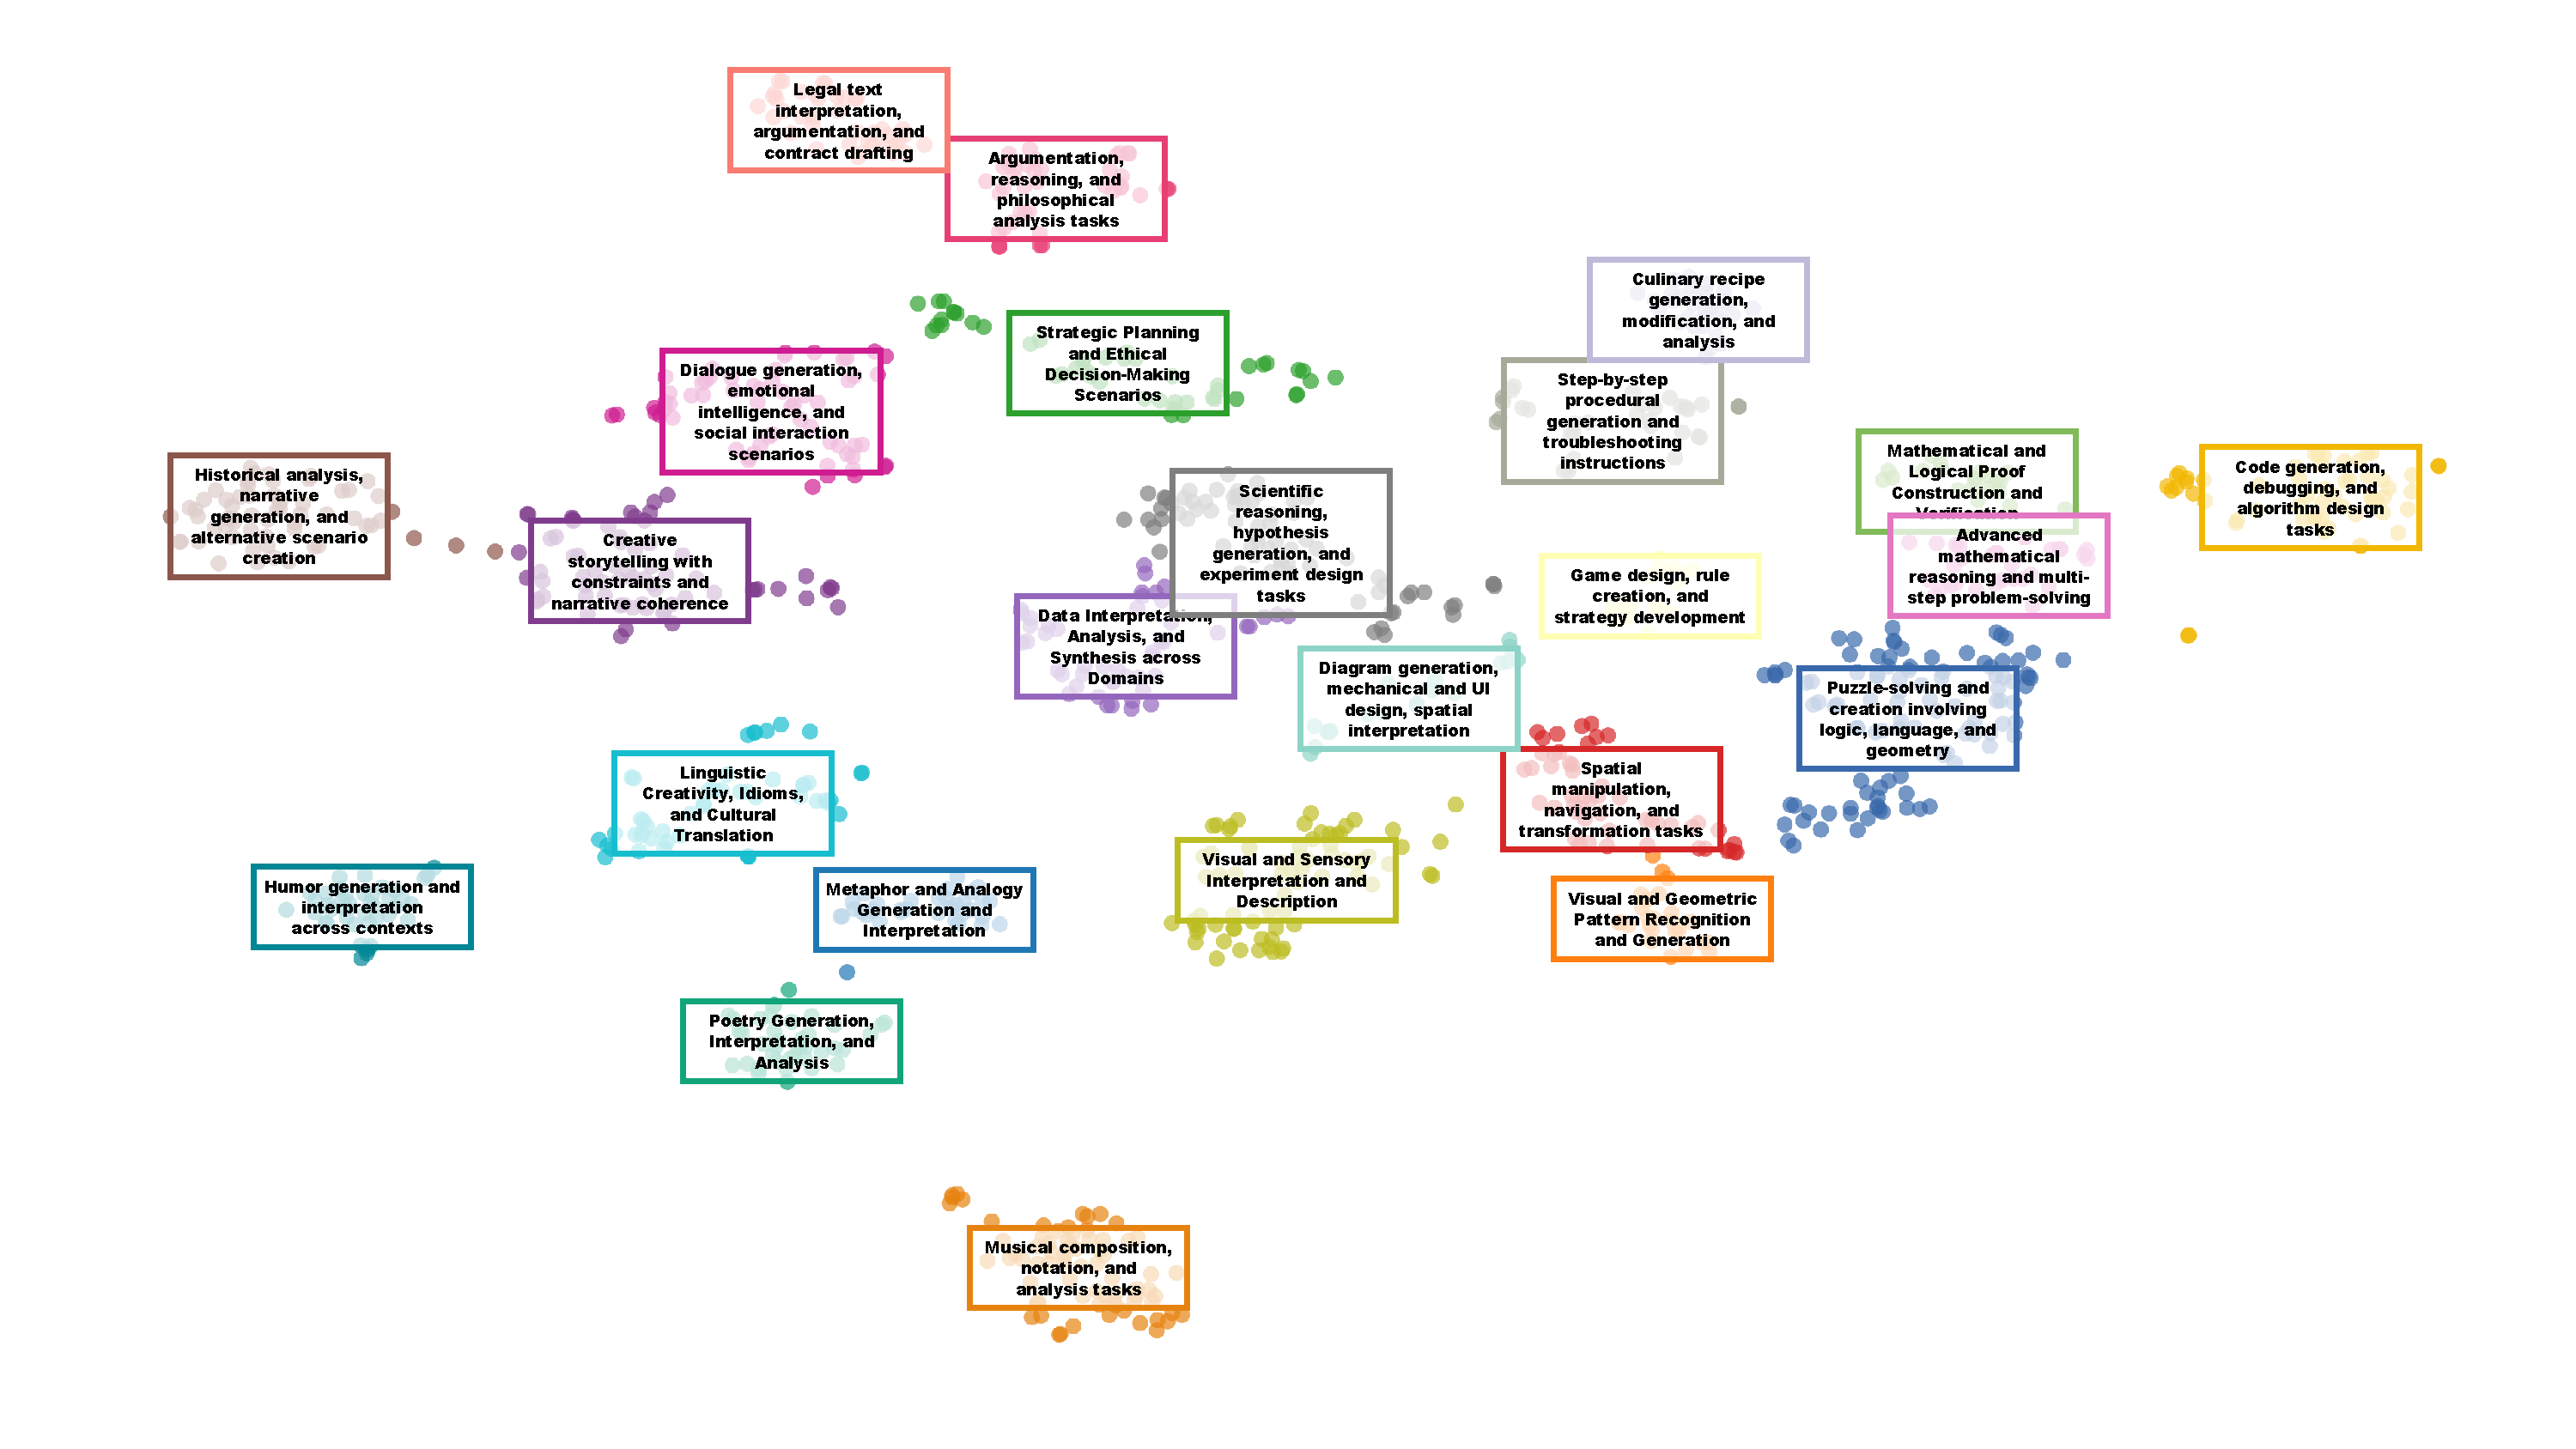
\includegraphics[width=1\textwidth,height=\textheight]{/Users/shengran/projects/ACD/reports/cluster_vis_gpt4_gpt4.pdf}
\caption{Visualization of task families discovered by ACD on GPT-4o
subject by GPT-4o scientist over 5000 generations.}\label{fig:cluster}
}
\end{figure}

\hypertarget{insights}{%
\subsection{Insights}\label{insights}}

\begin{itemize}
\tightlist
\item
  The LLM excels in tasks requiring procedural understanding and
  technical communication, particularly in
  \protect\hyperlink{step-by-step-procedural-generation-and-troubleshooting-instructions}{Step-by-step
  procedural generation and troubleshooting instructions}, where it
  achieves a high success rate in tasks like origami instructions,
  demonstrating strong spatial reasoning and instructional clarity.
\item
  In
  \protect\hyperlink{scientific-reasoning-hypothesis-generation-and-experiment-design-tasks}{Scientific
  reasoning, hypothesis generation, and experiment design tasks}, the
  model shows proficiency in scientific reasoning and simplifying
  complex concepts, although it struggles with experimental design for
  abstract phenomena, indicating a need for improved operationalization
  of scientific ideas.
\item
  The model's legal reasoning and document generation capabilities are
  highlighted in
  \protect\hyperlink{legal-text-interpretation-argumentation-and-contract-drafting}{Legal
  text interpretation, argumentation, and contract drafting}, where it
  effectively interprets legal texts and constructs arguments,
  suggesting its utility in legal research and document preparation.
\item
  Despite strengths in structured reasoning, the LLM struggles with
  dynamic and strategic tasks, as seen in
  \protect\hyperlink{game-design-rule-creation-and-strategy-development}{Game
  design, rule creation, and strategy development}, where it fails in
  complex pathfinding and chess strategy tasks, pointing to limitations
  in spatial reasoning and domain-specific adaptations.
\item
  The analysis of numerical data reveals high success rates in clusters
  involving scientific reasoning and historical analysis, suggesting
  strong interdisciplinary synthesis capabilities, but highlights
  weaknesses in advanced mathematical reasoning, indicating areas for
  improvement.
\end{itemize}

\hypertarget{surprising-capabilities}{%
\subsection{Surprising Capabilities}\label{surprising-capabilities}}

\begin{itemize}
\tightlist
\item
  The LLM's ability to generate coherent step-by-step instructions in
  \protect\hyperlink{step-by-step-procedural-generation-and-troubleshooting-instructions}{Step-by-step
  procedural generation and troubleshooting instructions}, particularly
  for tasks like origami, showcases a surprising proficiency in spatial
  reasoning and procedural communication, suggesting potential
  applications in education and technical writing.
\item
  In
  \protect\hyperlink{scientific-reasoning-hypothesis-generation-and-experiment-design-tasks}{Scientific
  reasoning, hypothesis generation, and experiment design tasks}, the
  model's capability to simplify complex scientific concepts into
  accessible explanations demonstrates a notable strength in scientific
  communication, although with limitations in experimental design.
\item
  The high success rate in legal reasoning tasks in
  \protect\hyperlink{legal-text-interpretation-argumentation-and-contract-drafting}{Legal
  text interpretation, argumentation, and contract drafting} reveals a
  surprising depth of understanding in legal principles and the ability
  to generate coherent legal documents, highlighting its utility in
  legal domains.
\end{itemize}

\hypertarget{surprising-failures}{%
\subsection{Surprising Failures}\label{surprising-failures}}

\begin{itemize}
\tightlist
\item
  The LLM's inability to effectively handle dynamic and strategic
  reasoning tasks, as evidenced in
  \protect\hyperlink{game-design-rule-creation-and-strategy-development}{Game
  design, rule creation, and strategy development}, where it struggles
  with pathfinding and chess strategy, indicates a significant
  limitation in adapting to dynamic environments and integrating spatial
  considerations.
\item
  In
  \protect\hyperlink{advanced-mathematical-reasoning-and-multi-step-problem-solving}{Advanced
  mathematical reasoning and multi-step problem-solving}, the model's
  lower success rate in advanced mathematical reasoning tasks, including
  complex mathematical modeling and symbolic manipulation, reveals a
  critical shortcoming in its mathematical understanding and
  problem-solving capabilities.
\item
  Despite strengths in abstract reasoning, the model's performance in
  \protect\hyperlink{mathematical-and-logical-proof-construction-and-verification}{Mathematical
  and Logical Proof Construction and Verification}, where it shows
  weaknesses in generating basic mathematical proofs, suggests an
  inconsistency in logical reasoning across different complexity levels.
\end{itemize}

\begin{figure}
\hypertarget{fig:radar}{%
\centering
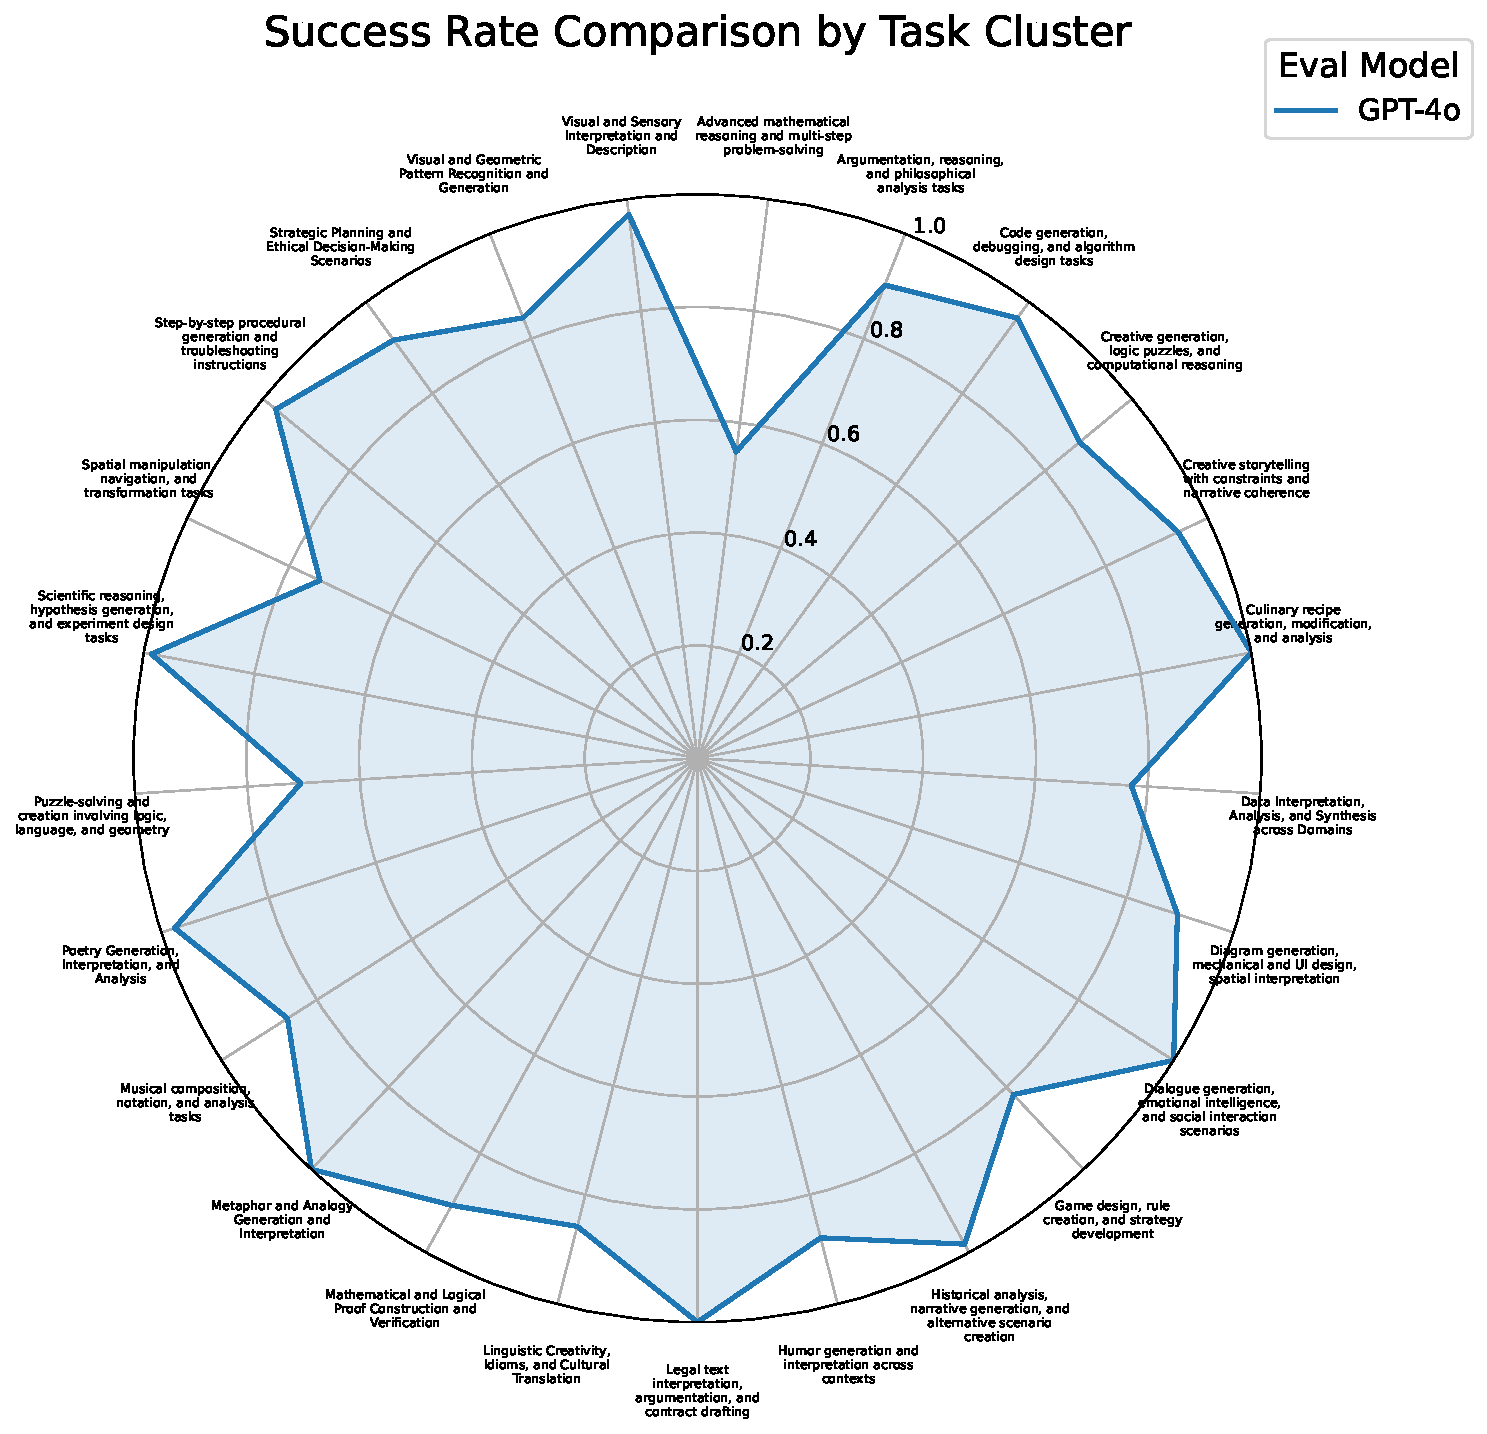
\includegraphics[width=0.55\textwidth,height=\textheight]{/Users/shengran/projects/ACD/reports/cluster_radar_gpt4_gpt4.pdf}
\caption{Success rates on each cluster of tasks.}\label{fig:radar}
}
\end{figure}

\hypertarget{data-insights}{%
\subsection{Data Insights}\label{data-insights}}

\begin{itemize}
\tightlist
\item
  The overall success rate of 87.57\% indicates strong performance
  across many clusters, yet significant variability suggests certain
  domains where the model excels versus those it struggles with.
\item
  Clusters with the highest success rates, such as
  \protect\hyperlink{scientific-reasoning-hypothesis-generation-and-experiment-design-tasks}{Scientific
  reasoning, hypothesis generation, and experiment design tasks}
  (97.75\%) and
  \protect\hyperlink{historical-analysis-narrative-generation-and-alternative-scenario-creation}{Historical
  analysis, narrative generation, and alternative scenario creation}
  (97.50\%), highlight the model's proficiency in interdisciplinary
  reasoning and historical analysis, suggesting effective synthesis and
  creative capabilities.
\item
  The notably lower success rate in
  \protect\hyperlink{advanced-mathematical-reasoning-and-multi-step-problem-solving}{Advanced
  mathematical reasoning and multi-step problem-solving} (56.13\%)
  underscores the LLM's limitations in handling complex mathematical
  tasks, pointing to an area that requires further enhancement and
  training.
\item
  The success rates across clusters reveal a pattern where the model
  performs well in structured and rule-based tasks but faces challenges
  in dynamic, strategic, and abstract problem-solving scenarios.
\end{itemize}

\newpage

\hypertarget{detailed-task-analysis}{%
\section{Detailed Task Analysis}\label{detailed-task-analysis}}

\hypertarget{step-by-step-procedural-generation-and-troubleshooting-instructions}{%
\subsection{Step-by-step procedural generation and troubleshooting
instructions}\label{step-by-step-procedural-generation-and-troubleshooting-instructions}}

\hypertarget{overview-1}{%
\subsubsection{Overview}\label{overview-1}}

\textbf{Capabilities}: Procedural understanding, technical
communication, and instructional clarity

\textbf{Number of Tasks}: 34

\textbf{Success Rate}: 92.94\%

\textbf{Difficulty Success Rates}: - moderate: 95.00\% - hard: 91.50\%

\textbf{Difficulty Percentages}: - moderate: 41.2\%

\begin{itemize}
\tightlist
\item
  hard: 58.8\%
\end{itemize}

\hypertarget{analysis}{%
\subsubsection{Analysis}\label{analysis}}

The LLM demonstrates strong procedural understanding and technical
communication skills, particularly in tasks requiring detailed
step-by-step instructions and spatial reasoning, as reflected by the
high success rates in origami-related tasks.

\textbf{Insights}:

The model excels in tasks demanding clear procedural instructions and
spatial understanding, such as origami, revealing strengths in tasks
that require detailed sequencing and visualization. This capability
suggests potential applications in technical writing and documentation
fields, although it may face challenges in more abstract or less
structured procedural tasks.

\hypertarget{task-examples}{%
\subsubsection{Task Examples}\label{task-examples}}

\hypertarget{example-1}{%
\paragraph{Example 1}\label{example-1}}

\begin{quote}
\textbf{Task}: origami\_instructions \textbf{Task Description}:
Interpret given origami instructions and generate new origami
instructions based on specified shapes. \textbf{Difficulty Level}: 4
(hard) \textbf{Instructions}: Your task is to interpret the following
origami instructions and describe the resulting shape. Provide your
description in plain text format.

Instructions: Fold a square paper in half diagonally to form a triangle.
Unfold, then fold the paper in half diagonally in the opposite direction
to form a triangle. Unfold, then fold the paper in half horizontally to
form a rectangle. Unfold, then fold the paper in half vertically to form
a rectangle. Unfold.

Ensure your description is clear and accurately represents the final
shape formed by following the instructions. \textbf{Model Response
Example}: The resulting shape is a square piece of paper with creases
forming an asterisk (*) pattern. The creases intersect at the center,
dividing the square into eight triangular sections. \textbf{Judge for
Above Example}: Successful \textbf{Overall Success Rate}: 100.0\%
\end{quote}

The LLM's ability to accurately interpret and describe the final shape
from origami instructions was surprising due to the spatial reasoning
required. This success indicates a robust capacity for understanding and
visualizing procedural instructions, suggesting potential strength in
similar complex procedural tasks.

\hypertarget{example-2}{%
\paragraph{Example 2}\label{example-2}}

\begin{quote}
\textbf{Task}: origami\_instructions\_generation \textbf{Task
Description}: Generate and interpret step-by-step origami instructions
to create specific origami models. \textbf{Difficulty Level}: 4 (hard)
\textbf{Instructions}: Your task is to generate step-by-step origami
instructions to create the specified origami model. Begin with the given
initial step and ensure that each step is clear, detailed, and
necessary. The final step should complete the origami model. Here is the
information about the task:

Goal Model: crane Initial Step: Start with a square piece of paper with
the colored side up.

Submit your instructions in plain text format. Use the following format
for each step: Step 1: {[}Description of step{]} Step 2: {[}Description
of step{]} \ldots{} Final Step: {[}Final description completing the
model{]}

\textbf{Model Response Example}: Step 1: Start with a square piece of
paper with the colored side up. Step 2: Fold the paper in half
diagonally to form a triangle, then unfold it. Step 3: Fold the paper in
half diagonally in the other direction to form a triangle, then unfold
it again. You should now have two creases forming an ``X.'' Step 4: Turn
the paper over so the white side (or the side without color) is facing
up. Step 5: Fold the paper in half horizontally to form a rectangle,
then unfold it. Step 6: Fold the paper in half vertically to form a
rectangle, then unfold it. You should now have a grid of creases. Step
7: Collapse the paper into a square base by bringing the horizontal and
vertical creases together, forming a smaller square with the open ends
at the bottom. Step 8: Rotate the square base so that it looks like a
diamond with the open ends pointing down. Step 9: Fold the right corner
of the top layer to the center crease, then fold the left corner of the
top layer to the center crease. The top layer should now have a kite
shape. Step 10: Fold the top triangle down over the kite shape, creasing
well, then unfold the last three folds. Step 11: Lift the bottom corner
of the top layer, then fold it upwards along the creases made in Step
10, forming a tall, narrow diamond shape. Flatten the sides. Step 12:
Flip the paper over and repeat Steps 9 to 11 on the other side. Step 13:
Fold the right corner of the top layer to the center crease, then fold
the left corner of the top layer to the center crease, forming a kite
shape. Step 14: Fold the top triangle down over the kite shape, creasing
well, then unfold the last three folds. Step 15: Lift the bottom corner
of the top layer and fold it upwards along the creases made in Step 14,
forming a tall, narrow diamond shape. Flatten the sides. Step 16: Fold
the right flap and the left flap towards the center, aligning with the
central crease, then fold the top triangle down over the flaps to crease
well, and then unfold. Step 17: Open up the flaps created in Step 16,
then squash fold the sides to form a diamond shape. Step 18: Flip the
paper over and repeat Steps 16 and 17 on the other side. Step 19: Fold
the bottom edge of the top layer to meet the center crease, forming a
narrow kite shape. Repeat on the other side. Step 20: Fold the top
triangle down over the narrow kite shape, creasing well, then unfold the
last three folds. Step 21: Lift the bottom corner of the top layer and
fold it upwards along the creases made in Step 20, forming a tall,
narrow diamond shape. Flatten the sides. Step 22: Flip the paper over
and repeat Step 21 on the other side. Step 23: Fold the top flaps down
on both sides to create the wings of the crane. Step 24: Fold the bottom
flaps upwards to form the neck and tail of the crane. Step 25: Fold the
tip of one of the bottom flaps down to form the crane's head. Final
Step: Pull the wings apart gently to give the crane its final shape and
make it three-dimensional. Adjust the neck and head as necessary. Your
origami crane is now complete! \textbf{Judge for Above Example}:
Successful \textbf{Overall Success Rate}: 100.0\%
\end{quote}

The LLM's successful generation of a comprehensive set of origami
instructions for a crane model was surprising given the complexity and
number of steps involved. This performance highlights the model's
capability to handle intricate procedural tasks with clarity and
thoroughness, which is impressive considering the potential for errors
in long sequences.

\hypertarget{scientific-reasoning-hypothesis-generation-and-experiment-design-tasks}{%
\subsection{Scientific reasoning, hypothesis generation, and experiment
design
tasks}\label{scientific-reasoning-hypothesis-generation-and-experiment-design-tasks}}

\hypertarget{overview-2}{%
\subsubsection{Overview}\label{overview-2}}

\textbf{Capabilities}: Scientific reasoning, experimental design,
creativity, explanatory skills

\textbf{Number of Tasks}: 71

\textbf{Success Rate}: 97.75\%

\textbf{Difficulty Success Rates}: - moderate: 100.00\% - hard: 97.46\%
- very hard: 98.57\%

\textbf{Difficulty Percentages}: - moderate: 7.0\%

\begin{itemize}
\item
  hard: 83.1\%
\item
  very hard: 9.9\%
\end{itemize}

\hypertarget{analysis-1}{%
\subsubsection{Analysis}\label{analysis-1}}

The LLM demonstrates strong proficiency in simplifying complex
scientific concepts but shows limitations in accurately designing
experiments that capture the core principles of these concepts. This
suggests a gap in the model's ability to fully understand and
operationalize abstract scientific ideas into concrete, illustrative
experiments, particularly for phenomena like quantum entanglement.

\textbf{Insights}:

The LLM excels at breaking down complex ideas into simpler terms, which
is a strength in communication. However, its limitations in conceptual
understanding become apparent in tasks requiring accurate experiment
design, especially for abstract topics. This suggests that while LLMs
can aid in educational contexts by providing explanations, they may
struggle with tasks requiring deep scientific reasoning and creativity
in experiment design. Further training or model adjustments may be
needed to enhance these capabilities.

\hypertarget{task-examples-1}{%
\subsubsection{Task Examples}\label{task-examples-1}}

\hypertarget{example-1-1}{%
\paragraph{Example 1}\label{example-1-1}}

\begin{quote}
\textbf{Task}: explain\_scientific\_concepts \textbf{Task Description}:
Explain complex scientific concepts in simple terms and design simple
experiments to demonstrate these concepts. \textbf{Difficulty Level}: 4
(hard) \textbf{Instructions}: Your task is to explain the following
scientific concept in simple terms and design a simple experiment to
demonstrate it:

Scientific Concept: Quantum Entanglement

\begin{enumerate}
\def\labelenumi{\arabic{enumi}.}
\tightlist
\item
  Provide a clear and simple explanation of the concept. Your
  explanation should be understandable to someone without a scientific
  background.
\item
  Design a simple experiment that can be conducted to demonstrate the
  concept. The experiment should include at least 3 steps and use
  materials commonly available at home or in a school lab.
\end{enumerate}

Ensure that your explanation is comprehensive and your experiment is
practical and illustrative of the concept. Provide your response in the
following format:

Explanation: {[}Your explanation{]} Experiment: {[}Your experiment
design{]} \textbf{Model Response Example}: Explanation: Quantum
entanglement is like a magical connection between two particles, such as
tiny bits of light called photons. Imagine you have two dice that are
magically linked together. If you roll one die and it lands on a six,
the other die will also show a six at the same time, no matter how far
apart they are. This connection is so special that even if one die is on
Earth and the other is on the Moon, they will still show the same result
instantly. Scientists find this very fascinating because it seems like
the two particles communicate faster than the speed of light, which is
something we still don't fully understand.

Experiment: To demonstrate the idea of quantum entanglement with a
simple analogy, you can use two identical pieces of paper and some
colored markers.

\begin{enumerate}
\def\labelenumi{\arabic{enumi}.}
\tightlist
\item
  \textbf{Materials Needed:}

  \begin{itemize}
  \tightlist
  \item
    Two identical pieces of paper
  \item
    Two sets of colored markers (at least three different colors)
  \item
    A friend or family member to help
  \end{itemize}
\item
  \textbf{Step-by-Step Process:}

  \begin{itemize}
  \tightlist
  \item
    \textbf{Step 1:} Sit down with your friend at a table. Each of you
    takes one piece of paper and one set of colored markers. Agree on
    which colors will represent different outcomes (e.g., red for heads,
    blue for tails, and green for a special outcome).
  \item
    \textbf{Step 2:} Decide together on a secret pattern or rule for
    coloring the paper. For example, you might decide that if you color
    a circle in the center with red, your friend should color a square
    in the corner with red, and so on for the other colors.
  \item
    \textbf{Step 3:} Without looking at each other's papers, follow the
    agreed-upon pattern and color your papers. After finishing, compare
    the papers. You'll see that the patterns match exactly,
    demonstrating how the ``entanglement'' kept the results correlated,
    even though you worked separately.
  \end{itemize}
\end{enumerate}

This experiment shows how two things can be connected in a way that
their states are dependent on each other, similar to how entangled
particles behave. \textbf{Judge for Above Example}: Failed
\textbf{Overall Success Rate}: 50.0\%
\end{quote}

The failure in this example is surprising because the model's analogy
for quantum entanglement was relatively accessible and understandable,
yet the experimental design missed the mark entirely. This highlights a
disconnect between the model's surface-level understanding and its
ability to apply that understanding in practical, scientifically
accurate ways.

\hypertarget{strategic-planning-and-ethical-decision-making-scenarios}{%
\subsection{Strategic Planning and Ethical Decision-Making
Scenarios}\label{strategic-planning-and-ethical-decision-making-scenarios}}

\hypertarget{overview-3}{%
\subsubsection{Overview}\label{overview-3}}

\textbf{Capabilities}: strategic thinking, ethical reasoning,
decision-making

\textbf{Number of Tasks}: 48

\textbf{Success Rate}: 88.54\%

\textbf{Difficulty Success Rates}: - moderate: 76.67\% - hard: 88.16\% -
very hard: 95.71\%

\textbf{Difficulty Percentages}: - moderate: 6.2\%

\begin{itemize}
\item
  hard: 79.2\%
\item
  very hard: 14.6\%
\end{itemize}

\hypertarget{analysis-2}{%
\subsubsection{Analysis}\label{analysis-2}}

The LLM demonstrates strong capabilities in strategic thinking and
ethical reasoning, particularly in complex moral dilemmas, but shows
limitations in tasks requiring precise optimization and real-time
resource management. Its ability to apply ethical principles effectively
contrasts with its struggles in computationally intensive tasks.

\textbf{Insights}:

The LLM excels in ethical reasoning and strategic planning,
demonstrating a deep understanding of abstract principles. However, its
limitations in optimization and real-time management tasks suggest a
need for improvement in handling detailed, computationally intensive
problems. This aligns with broader questions about LLMs' ability to
perform tasks requiring precise calculations and dynamic adjustments,
areas where human expertise may still be superior.

\hypertarget{task-examples-2}{%
\subsubsection{Task Examples}\label{task-examples-2}}

\hypertarget{example-1-2}{%
\paragraph{Example 1}\label{example-1-2}}

\begin{quote}
\textbf{Task}: ethical\_decision\_making \textbf{Task Description}:
Generate solutions to ethical dilemmas and evaluate the ethics of given
actions. \textbf{Difficulty Level}: 5 (very hard) \textbf{Instructions}:
Your task is to generate a solution to the following ethical dilemma:

You are a doctor with five patients in critical condition. Each needs a
different organ transplant to survive, and there are no available
donors. A healthy young traveler comes to you for a routine check-up.
You realize he is a perfect match for all five patients. Should you
sacrifice the traveler to save the five patients?

Provide a detailed explanation of your solution, including the ethical
principles and reasoning behind your decision. Ensure your response is
comprehensive and considers multiple perspectives. Your response should
be structured in a step-by-step format. \textbf{Model Response Example}:
1. \textbf{Introduction of Ethical Dilemma}: - The dilemma involves
choosing between sacrificing one healthy individual to save five
critically ill patients. - This situation pits utilitarian ethics
(maximizing overall well-being) against deontological ethics (duty and
rights-based ethics).

\begin{enumerate}
\def\labelenumi{\arabic{enumi}.}
\setcounter{enumi}{1}
\tightlist
\item
  \textbf{Utilitarian Perspective}:

  \begin{itemize}
  \tightlist
  \item
    \textbf{Principle}: Actions are right if they promote the greatest
    happiness for the greatest number.
  \item
    \textbf{Reasoning}: Sacrificing one person to save five would
    maximize overall well-being and the total number of lives saved.
  \end{itemize}
\item
  \textbf{Deontological Perspective}:

  \begin{itemize}
  \tightlist
  \item
    \textbf{Principle}: Actions are right or wrong in themselves,
    regardless of the consequences.
  \item
    \textbf{Reasoning}: It is inherently wrong to kill an innocent
    person, regardless of the potential benefits.
  \end{itemize}
\item
  \textbf{Medical Ethics Principles (Four Principles Approach)}:

  \begin{itemize}
  \tightlist
  \item
    \textbf{Autonomy}: Respecting the traveler's autonomy means
    acknowledging his right to make decisions about his own body.
  \item
    \textbf{Beneficence}: Aiming to do good for the patients.
  \item
    \textbf{Non-maleficence}: ``Do no harm'' -- harming the traveler to
    save the patients violates this principle.
  \item
    \textbf{Justice}: Fair distribution of resources and ensuring no
    individual is unfairly sacrificed for others.
  \end{itemize}
\item
  \textbf{Legal and Social Considerations}:

  \begin{itemize}
  \tightlist
  \item
    \textbf{Legal}: Non-consensual organ harvesting is illegal and
    constitutes murder.
  \item
    \textbf{Social Trust}: Sacrificing the traveler would erode public
    trust in the medical profession and could lead to societal fear and
    loss of faith in healthcare providers.
  \end{itemize}
\item
  \textbf{Balancing the Perspectives}:

  \begin{itemize}
  \tightlist
  \item
    While utilitarianism suggests sacrificing the traveler, the
    overwhelming principles of deontology, medical ethics, and legal
    considerations argue against it.
  \item
    The traveler's right to life and bodily autonomy cannot be
    overridden by the needs of the patients.
  \end{itemize}
\item
  \textbf{Conclusion}:

  \begin{itemize}
  \tightlist
  \item
    \textbf{Decision}: Do not sacrifice the healthy traveler.
  \item
    \textbf{Justification}: Upholding ethical principles such as respect
    for autonomy, non-maleficence, and legal standards is crucial. The
    traveler's rights and the integrity of the medical profession must
    be preserved.
  \end{itemize}
\end{enumerate}

Answer: Do not sacrifice the traveler to save the five patients.
\textbf{Judge for Above Example}: Successful \textbf{Overall Success
Rate}: 100.0\%
\end{quote}

The success in Example 2 is surprising because it involves a very
nuanced ethical dilemma that requires balancing multiple ethical
theories and principles. The LLM successfully navigates this complexity,
highlighting its capability to handle abstract, theoretical reasoning
with clarity and depth.

\hypertarget{example-2-1}{%
\paragraph{Example 2}\label{example-2-1}}

\begin{quote}
\textbf{Task}: ethical\_reasoning\_moral\_dilemmas \textbf{Task
Description}: Analyze and provide solutions to moral dilemmas, offering
rational justifications and demonstrating ethical understanding.
\textbf{Difficulty Level}: 5 (very hard) \textbf{Instructions}: Your
task is to analyze and provide a solution to the following moral
dilemma: `A train is heading towards five workers on the track. You are
standing next to a lever that can switch the train to another track,
where there is one worker. Do you pull the lever?' Your response should
include:

\begin{enumerate}
\def\labelenumi{\arabic{enumi}.}
\item
  A clear statement of your decision or proposed solution.
\item
  A detailed explanation of the ethical principles and reasoning behind
  your decision.
\item
  Consideration of potential objections to your decision and your
  responses to those objections.
\item
  Any relevant examples or analogies that support your reasoning.
  \textbf{Model Response Example}: I would pull the lever to switch the
  train to the other track where there is one worker.
\item
  My decision is to pull the lever.
\item
  The ethical principle behind my decision is utilitarianism, which
  advocates for actions that maximize overall happiness or well-being.
  In this scenario, pulling the lever results in the least harm by
  saving five lives at the expense of one. The core idea is to minimize
  overall suffering, and since five lives have a greater combined value
  than one, the utilitarian approach would prioritize saving the greater
  number of people.
\item
  Potential objections to my decision include:

  \begin{itemize}
  \tightlist
  \item
    \textbf{The moral status of actively causing harm:} Some argue that
    actively diverting the train makes me directly responsible for the
    death of the one worker, while not acting would mean I am merely a
    bystander to the deaths of the five workers. My response is that
    inaction in this scenario also constitutes a moral choice with
    significant consequences. By not pulling the lever, I allow the
    greater harm to occur. Therefore, the moral responsibility remains
    regardless of action or inaction.
  \item
    \textbf{Violation of individual rights:} Another objection is that
    pulling the lever violates the individual rights of the one worker.
    My response is that while individual rights are important, in
    extreme situations where lives are at stake, a utilitarian approach
    provides a compelling reason to act in a way that achieves the best
    overall outcome.
  \item
    \textbf{Slippery slope argument:} Some may argue that justifying
    harm to one person for the greater good could lead to dangerous
    precedents. My response is that this specific scenario is an
    extraordinary situation that necessitates a particular moral
    consideration, and such decisions should be carefully evaluated
    within their unique context rather than generalized.
  \end{itemize}
\item
  Relevant examples and analogies:

  \begin{itemize}
  \tightlist
  \item
    \textbf{The classic trolley problem:} This scenario is a direct
    application of the trolley problem, a well-known ethical thought
    experiment used to explore moral dilemmas and utilitarian
    principles.
  \item
    \textbf{Medical triage:} In emergency medicine, doctors often have
    to make similar decisions where they prioritize treatment for those
    who have the best chance of survival, which aligns with the
    utilitarian approach of maximizing overall well-being.
  \end{itemize}
\end{enumerate}

In conclusion, while the decision to pull the lever is difficult and
involves complex moral considerations, the utilitarian framework
provides a reasoned approach to minimizing harm and saving the greatest
number of lives. \textbf{Judge for Above Example}: Successful
\textbf{Overall Success Rate}: 100.0\%
\end{quote}

Example 3's success is notable due to the difficulty of applying
utilitarian principles effectively in a classic moral dilemma. The LLM's
ability to articulate and justify its decision-making process, while
addressing potential objections, showcases its strong ethical reasoning
capabilities.

\hypertarget{example-3}{%
\paragraph{Example 3}\label{example-3}}

\begin{quote}
\textbf{Task}: combinatorial\_optimization\_scheduling \textbf{Task
Description}: Solve scheduling problems by optimizing resource
allocation and meeting specified constraints. \textbf{Difficulty Level}:
4 (hard) \textbf{Instructions}: Your task is to solve the following
scheduling problem by optimizing resource allocation and meeting the
specified constraints:

A factory has 5 machines and 8 tasks to complete. Each task can only be
performed by a specific set of machines, and each machine can only
handle one task at a time. The goal is to assign tasks to machines in
such a way that all tasks are completed in the shortest possible time.
The following are the processing times (in hours) for each task on each
machine:

Machine 1: Task 1 (3), Task 2 (2) Machine 2: Task 1 (4), Task 3 (1)
Machine 3: Task 2 (5), Task 4 (3) Machine 4: Task 3 (2), Task 5 (4),
Task 6 (1) Machine 5: Task 4 (1), Task 6 (2), Task 7 (3), Task 8 (2)

Tasks 1 and 2 must be completed before Task 4 can start. Tasks 3 and 5
must be completed before Task 7 can start.

Your response should include: 1. A clear description of the optimal
schedule, including which tasks or sessions are assigned to which
resources (machines or rooms) and the order in which they are performed.
2. The total time required to complete all tasks or sessions.

Ensure your response is well-organized, logically structured, and
includes all required components in a clear manner. \textbf{Model
Response Example}: 1. Optimal Schedule: - Machine 1: Task 1 (0-3 hours),
Task 2 (3-5 hours) - Machine 2: Task 3 (0-1 hour) - Machine 3: No tasks
assigned - Machine 4: Task 5 (0-4 hours), Task 6 (4-5 hours) - Machine
5: Task 4 (5-6 hours), Task 7 (6-9 hours), Task 8 (9-11 hours) 2. Total
time required to complete all tasks: 11 hours \textbf{Judge for Above
Example}: Failed \textbf{Overall Success Rate}: 50.0\%
\end{quote}

The failure in Example 4 is surprising given the LLM's overall high
success rate and suggests a limitation in handling complex scheduling
problems that require optimal resource allocation and constraint
satisfaction, areas typically requiring detailed computational
strategies.

\hypertarget{example-4}{%
\paragraph{Example 4}\label{example-4}}

\begin{quote}
\textbf{Task}: real\_time\_resource\_management \textbf{Task
Description}: Manage a resource in a simulated environment by making
decisions based on changing conditions. \textbf{Difficulty Level}: 4
(hard) \textbf{Instructions}: Your task is to manage the water levels in
a reservoir to ensure that the demand is met without overflowing. You
will receive real-time updates on the incoming flow, demand, and current
reservoir level. You have 60 seconds to make decisions and maintain the
balance.

Initial Conditions: - Reservoir Level: 50 units - Incoming Flow: 10
units per second - Demand: 5 units per second - Time Limit: 60 seconds

Dynamic Conditions (over time): - Time Intervals: {[}0, 10, 20, 30, 40,
50, 60{]} - Incoming Flow: {[}10, 15, 20, 10, 5, 8, 12{]} - Demand:
{[}5, 10, 8, 6, 4, 7, 9{]}

Make decisions and submit your actions at each time interval in the
format: `Time: {[}Time Interval{]}, Action: {[}Your Action{]}.' Your
actions can be `Increase Outflow,' `Decrease Outflow,' or `Maintain
Outflow.' Provide your response in plain text format. Here is an
example:

Time: 10, Action: Increase Outflow Time: 20, Action: Decrease Outflow
Time: 30, Action: Maintain Outflow

\textbf{Model Response Example}: Time: 10, Action: Increase Outflow
Time: 20, Action: Increase Outflow Time: 30, Action: Increase Outflow
Time: 40, Action: Maintain Outflow Time: 50, Action: Increase Outflow
Time: 60, Action: Maintain Outflow \textbf{Judge for Above Example}:
Failed \textbf{Overall Success Rate}: 0.0\%
\end{quote}

Example 5 reveals a significant limitation in real-time decision-making
and dynamic resource management. Despite the LLM's proficiency in
strategic planning, it struggles to adapt to changing conditions and
optimize resource allocation effectively under time constraints.

\hypertarget{example-5}{%
\paragraph{Example 5}\label{example-5}}

\begin{quote}
\textbf{Task}: create\_schedule \textbf{Task Description}: Generate a
detailed schedule given a set of tasks with specific constraints.
\textbf{Difficulty Level}: 4 (hard) \textbf{Instructions}: Your task is
to create a detailed schedule for the following tasks within the given
time frame. Each task has a specified duration and may depend on the
completion of other tasks. The schedule should be feasible, respecting
all task dependencies, and fitting within the specified start and end
times. Provide your schedule as a list of tuples (task\_name,
start\_time, end\_time), where start\_time and end\_time are formatted
as HH:MM.

Tasks: {[}\{`name': `Task A,' `duration': 2, `dependencies': {[}{]}\},
\{`name': `Task B,' `duration': 1, `dependencies': {[}`Task A'{]}\},
\{`name': `Task C,' `duration': 3, `dependencies': {[}`Task A'{]}\}{]}

Start Time: 09:00 End Time: 17:00 \textbf{Model Response Example}:
{[}(`Task A,' `09:00,' `11:00'), (`Task B,' `11:00,' `12:00'), (`Task
C,' `11:00,' `14:00'){]} \textbf{Judge for Above Example}: Failed
\textbf{Overall Success Rate}: 30.0\%
\end{quote}

The failure in Example 6 underscores the LLM's difficulty with
scheduling tasks that involve dependencies and precise time management,
indicating a gap in its ability to translate task requirements into
feasible schedules that respect constraints.

\hypertarget{legal-text-interpretation-argumentation-and-contract-drafting}{%
\subsection{Legal text interpretation, argumentation, and contract
drafting}\label{legal-text-interpretation-argumentation-and-contract-drafting}}

\hypertarget{overview-4}{%
\subsubsection{Overview}\label{overview-4}}

\textbf{Capabilities}: Legal reasoning, document generation, and
argument construction

\textbf{Number of Tasks}: 41

\textbf{Success Rate}: 97.07\%

\textbf{Difficulty Success Rates}: - hard: 96.11\% - very hard: 97.83\%

\textbf{Difficulty Percentages}: - hard: 43.9\%

\begin{itemize}
\tightlist
\item
  very hard: 56.1\%
\end{itemize}

\hypertarget{analysis-3}{%
\subsubsection{Analysis}\label{analysis-3}}

The LLM demonstrates advanced capabilities in legal text interpretation,
document generation, and argument construction, achieving high success
rates even in very difficult tasks. This performance suggests a strong
understanding of legal principles, structured reasoning, and the ability
to produce coherent legal documents.

\textbf{Insights}:

The examples reveal the LLM's proficiency in legal document drafting and
argumentation, showing that it can comprehend and apply legal principles
effectively to generate structured and legally sound responses. This
suggests potential applications in legal research, document preparation,
and preliminary case analysis, but also underscores the importance of
human oversight to verify accuracy and ensure ethical considerations are
met.

\hypertarget{task-examples-3}{%
\subsubsection{Task Examples}\label{task-examples-3}}

\hypertarget{example-1-3}{%
\paragraph{Example 1}\label{example-1-3}}

\begin{quote}
\textbf{Task}: legal\_document\_generation \textbf{Task Description}:
Generate a coherent and legally sound document based on provided legal
clauses and requirements. \textbf{Difficulty Level}: 5 (very hard)
\textbf{Instructions}: Your task is to generate a coherent and legally
sound document based on the following provided legal clauses and
requirements:

\begin{itemize}
\tightlist
\item
  This Agreement shall commence on the Effective Date and shall continue
  in full force and effect until terminated in accordance with the terms
  of this Agreement.
\item
  Either Party may terminate this Agreement upon providing thirty (30)
  days' written notice to the other Party.
\item
  Upon termination of this Agreement, each Party shall return or destroy
  all Confidential Information of the other Party in its possession.
\end{itemize}

Requirements: Create a termination notice for this agreement, ensuring
that it includes the reason for termination and complies with the
provided clauses.

Ensure that your document is clear, accurate, and adheres to the
provided clauses. Provide your document in plain text format. Your
response should be structured as follows:

{[}Document Title{]} {[}Body of the document{]} \textbf{Model Response
Example}: Termination Notice

Dear {[}Recipient's Name{]},

This letter serves as formal written notice pursuant to the terms of the
Agreement effective {[}Effective Date{]}, between {[}Your Company
Name{]} (``We'' or ``Our'') and {[}Recipient's Company Name{]} (``You''
or ``Your''), that We are terminating the Agreement.

Reason for Termination: {[}State the reason for termination, e.g., ``Due
to the recent changes in our business operations, we have decided to
discontinue the services provided under this Agreement.''{]}

In accordance with the terms of the Agreement, this termination shall
take effect thirty (30) days from the date of this notice, which is
{[}Date of Notice{]}.

Upon termination of the Agreement, We request that You return or destroy
all Confidential Information in Your possession belonging to Us.
Likewise, We will ensure the return or destruction of all Confidential
Information belonging to You.

We appreciate the cooperation and understanding in this matter.

Sincerely,

{[}Your Name{]}\\
{[}Your Position{]}\\
{[}Your Company Name{]}\\
{[}Your Contact Information{]} \textbf{Judge for Above Example}:
Successful \textbf{Overall Success Rate}: 100.0\%
\end{quote}

The success in generating a termination notice that adheres to complex
legal requirements is surprising because it demonstrates the LLM's
ability to interpret and apply specific legal clauses accurately. This
suggests that the LLM can handle nuanced legal language and formal
document structures effectively.

\hypertarget{example-2-2}{%
\paragraph{Example 2}\label{example-2-2}}

\begin{quote}
\textbf{Task}: legal\_argumentation\_and\_analysis \textbf{Task
Description}: Generate a legal argument based on given facts and analyze
a provided legal argument to identify its strengths and weaknesses.
\textbf{Difficulty Level}: 5 (very hard) \textbf{Instructions}: Your
task is to generate a legal argument based on the following facts:

Facts: A person was injured in a car accident caused by another driver's
negligence. The injured party is seeking compensation for medical
expenses, lost wages, and pain and suffering. Draft a legal argument to
support the injured party's claim for compensation.

Ensure that your argument is logically structured, based on legal
principles, and supports the injured party's claim for compensation.
Provide your argument in plain text format.

Format your response as follows: 1. Introduction: {[}Your
introduction{]} 2. Legal Principles: {[}Legal principles supporting the
argument{]} 3. Application: {[}Application of legal principles to the
facts{]} 4. Conclusion: {[}Your conclusion{]} \textbf{Model Response
Example}: 1. Introduction: The injured party in this case seeks
compensation for injuries sustained in a car accident caused by another
driver's negligence. The claim includes demands for medical expenses,
lost wages, and pain and suffering. This legal argument will demonstrate
that the injured party is entitled to full compensation based on
established legal principles of negligence and liability.

\begin{enumerate}
\def\labelenumi{\arabic{enumi}.}
\setcounter{enumi}{1}
\tightlist
\item
  Legal Principles: Under tort law, particularly the principles
  governing negligence, an injured party is entitled to compensation if
  it can be proven that the other party owed a duty of care, breached
  that duty, and caused the injury as a direct result of the breach.
  Specifically:

  \begin{itemize}
  \tightlist
  \item
    Duty of Care: All drivers have a legal obligation to drive with
    reasonable care to avoid harming others.
  \item
    Breach of Duty: A breach occurs when a driver fails to act with the
    reasonable care expected under the circumstances.
  \item
    Causation: The breach must be the proximate cause of the injury.
  \item
    Damages: The injured party must have suffered actual harm or loss
    that can be compensated.
  \end{itemize}
\item
  Application: Applying these principles to the present facts:

  \begin{itemize}
  \tightlist
  \item
    Duty of Care: The defendant, as a driver on public roads, owed a
    duty of care to all other road users, including the injured party.
  \item
    Breach of Duty: The defendant breached this duty by driving
    negligently. Evidence of negligence may include traffic violations,
    reckless driving, or failure to adhere to traffic signals.
  \item
    Causation: The negligent actions of the defendant directly caused
    the car accident, leading to the injuries sustained by the injured
    party. This can be supported by eyewitness testimony, police
    reports, and accident scene analysis.
  \item
    Damages: The injured party has incurred significant medical expenses
    as a result of the injuries. Additionally, the injured party has
    lost wages due to the inability to work while recovering and has
    endured considerable pain and suffering. Documented medical bills,
    employment records, and personal testimony provide evidence of these
    damages.
  \end{itemize}
\item
  Conclusion: Based on the aforementioned legal principles and their
  application to the facts of this case, it is clear that the injured
  party is entitled to compensation. The defendant's negligent actions
  breached the duty of care owed to the injured party, directly causing
  the accident and subsequent injuries. Therefore, the injured party
  should be awarded compensation for medical expenses, lost wages, and
  pain and suffering to make them whole again. \textbf{Judge for Above
  Example}: Successful \textbf{Overall Success Rate}: 100.0\%
\end{enumerate}
\end{quote}

The LLM's ability to construct a detailed legal argument based on a
negligence scenario is impressive. It effectively applies legal
principles to support the injured party's claim, indicating a strong
grasp of legal reasoning and the ability to synthesize information into
a persuasive argument.

\hypertarget{example-3-1}{%
\paragraph{Example 3}\label{example-3-1}}

\begin{quote}
\textbf{Task}: legal\_argumentation \textbf{Task Description}: Analyze a
legal scenario and construct a coherent legal argument based on
specified laws and precedents. \textbf{Difficulty Level}: 5 (very hard)
\textbf{Instructions}: Your task is to analyze the given legal scenario
and construct a coherent legal argument based on the specified laws and
precedents.

Scenario: A company has been accused of violating environmental
regulations by dumping toxic waste into a river. The company argues that
the waste was within legal limits and that they have followed all
required procedures.

Laws: Environmental Protection Act Section 5, Clean Water Act Section
401 Precedents: United States v. Riverside Bayview Homes, Inc., Friends
of the Earth, Inc.~v. Laidlaw Environmental Services, Inc.

Your argument should be well-structured, logically coherent, and
reference the relevant laws and precedents. Provide your response in the
following format:

\begin{enumerate}
\def\labelenumi{\arabic{enumi}.}
\item
  Introduction: {[}Brief introduction of the scenario{]}
\item
  Legal Analysis: {[}Detailed legal analysis referencing the specified
  laws and precedents{]}
\item
  Conclusion: {[}Summary of your argument and conclusion{]}
  \textbf{Model Response Example}:
\item
  Introduction: The present scenario involves a company accused of
  violating environmental regulations by allegedly dumping toxic waste
  into a river. The company's defense is that the waste was within legal
  limits and that they have adhered to all required procedures. This
  argument demands an analysis based on the Environmental Protection Act
  Section 5, the Clean Water Act Section 401, and relevant precedents.
\item
  Legal Analysis: The Environmental Protection Act (EPA) Section 5
  mandates that any waste disposal must not harm the environment,
  specifying stringent limits on the toxicity of waste released into
  natural water bodies. The Clean Water Act (CWA) Section 401 requires
  that any discharge into navigable waters must obtain a certification
  that the discharge complies with the Act's provisions, ensuring that
  water quality standards are not violated.
\end{enumerate}

In United States v. Riverside Bayview Homes, Inc., the Supreme Court
held that the protection of water bodies extends to adjacent wetlands,
emphasizing the broad scope of the Clean Water Act in safeguarding water
quality. This precedent signifies that any activity potentially
impacting water bodies, including adjacent areas, falls under strict
scrutiny.

In Friends of the Earth, Inc.~v. Laidlaw Environmental Services, Inc.,
the Court ruled that compliance with permit limits does not absolve a
company from liability if the discharge still harms the environment.
This case underscores that merely adhering to procedural requirements
does not protect against liability if environmental harm occurs.

Applying these principles, the company must demonstrate that its waste
disposal did not harm the river's water quality, beyond mere procedural
compliance. Even if the waste was within legal limits and procedures
were followed, the company could still be liable under the Clean Water
Act if the waste negatively impacted the river's ecosystem. The broad
interpretation of environmental protection laws as established in
Riverside Bayview Homes and Laidlaw Environmental Services supports this
view.

\begin{enumerate}
\def\labelenumi{\arabic{enumi}.}
\setcounter{enumi}{2}
\tightlist
\item
  Conclusion: In conclusion, while the company argues that it complied
  with legal limits and procedures, this does not necessarily absolve it
  of liability under the Environmental Protection Act and Clean Water
  Act. The precedents set by United States v. Riverside Bayview Homes,
  Inc.~and Friends of the Earth, Inc.~v. Laidlaw Environmental Services,
  Inc.~indicate that the company must ensure its actions do not harm the
  environment, beyond mere procedural adherence. Therefore, a thorough
  investigation into the actual environmental impact of the waste
  disposal is required to determine the company's liability.
  \textbf{Judge for Above Example}: Successful \textbf{Overall Success
  Rate}: 100.0\%
\end{enumerate}
\end{quote}

The LLM's success in analyzing a legal scenario and referencing
appropriate laws and precedents to construct a coherent argument is
noteworthy. It demonstrates an understanding of both statutory
interpretation and case law application, highlighting its capability to
integrate complex legal concepts.

\hypertarget{diagram-generation-mechanical-and-ui-design-spatial-interpretation}{%
\subsection{Diagram generation, mechanical and UI design, spatial
interpretation}\label{diagram-generation-mechanical-and-ui-design-spatial-interpretation}}

\hypertarget{overview-5}{%
\subsubsection{Overview}\label{overview-5}}

\textbf{Capabilities}: visualization, spatial reasoning, technical
design, creativity

\textbf{Number of Tasks}: 19

\textbf{Success Rate}: 86.32\%

\textbf{Difficulty Success Rates}: - moderate: 86.67\% - hard: 88.46\% -
very hard: 76.67\%

\textbf{Difficulty Percentages}: - moderate: 15.8\%

\begin{itemize}
\item
  hard: 68.4\%
\item
  very hard: 15.8\%
\end{itemize}

\hypertarget{analysis-4}{%
\subsubsection{Analysis}\label{analysis-4}}

The LLM demonstrates strong capabilities in spatial reasoning, technical
diagram generation, and qualitative design critique. However,
limitations are evident in precise quantitative calculations and
mechanical comprehension tasks. These insights suggest the LLM excels in
conceptual and qualitative understanding but struggles with tasks
requiring exact numerical precision.

\textbf{Insights}:

The LLM's strengths lie in spatial reasoning and qualitative critique,
with limitations in precise quantitative calculations. This suggests the
model is effective in understanding and generating complex mechanical
and design concepts but struggles with tasks requiring exact numerical
precision, highlighting the need for improved quantitative reasoning
capabilities.

\hypertarget{task-examples-4}{%
\subsubsection{Task Examples}\label{task-examples-4}}

\hypertarget{example-1-4}{%
\paragraph{Example 1}\label{example-1-4}}

\begin{quote}
\textbf{Task}: spatial\_mechanical\_reasoning \textbf{Task Description}:
Solve problems that involve understanding and manipulating
three-dimensional objects, predicting outcomes of movements, and fitting
parts together. \textbf{Difficulty Level}: 4 (hard)
\textbf{Instructions}: Your task is to solve the following problem based
on the given context:

You are given a description of a three-dimensional object composed of
interlocking parts. The object is a simple mechanical toy consisting of
a base, a rotating gear, and a lever. The base is a rectangular block
with a hole for the gear's axle. The gear is a circular disk with teeth
along its edge and an axle that fits into the base. The lever is a flat
bar with a notch that fits over one of the gear's teeth. When the gear
rotates, the notch in the lever causes the lever to move up and down.
Describe how the parts fit together and predict the movement of the
lever when the gear is rotated.

Ensure that your solution meets the following requirements: Provide a
detailed description of how the parts fit together and explain the
movement of the lever when the gear is rotated. Include a step-by-step
explanation of the mechanical interactions between the parts.

Provide a detailed, step-by-step explanation of your solution, including
all mechanical interactions, shapes, and orientations. Your response
should be clear, logical, and comprehensive. Format your response as
follows:

\begin{enumerate}
\def\labelenumi{\arabic{enumi}.}
\tightlist
\item
  Problem Statement: {[}Brief summary of the problem{]}
\item
  Solution Approach: {[}Your approach to solving the problem{]}
\item
  Mechanical Interactions: {[}Detailed explanation of interactions
  between parts{]}
\item
  Conclusion: {[}Your final solution and reasoning{]} \textbf{Model
  Response Example}: The base, gear, and lever fit together to form a
  mechanical toy where the base supports the rotating gear. The gear's
  teeth engage with the notch in the lever, causing the lever to move up
  and down as the gear rotates. This interaction results in a continuous
  oscillating motion of the lever driven by the rotation of the gear.
  \textbf{Judge for Above Example}: Successful \textbf{Overall Success
  Rate}: 60.0\%
\end{enumerate}
\end{quote}

The success in spatial mechanical reasoning was surprising given the
complexity involved in predicting mechanical interactions. This reveals
the LLM's strong capability in understanding spatial arrangements and
predicting outcomes, although the overall success rate indicates
inconsistency in these tasks.

\hypertarget{example-2-3}{%
\paragraph{Example 2}\label{example-2-3}}

\begin{quote}
\textbf{Task}: mechanical\_comprehension \textbf{Task Description}:
Interpret mechanical diagrams and solve related problems, testing
spatial reasoning and understanding of mechanical principles.
\textbf{Difficulty Level}: 4 (hard) \textbf{Instructions}: Your task is
to solve the following problem related to a mechanical diagram:

A lever system where a 2-meter-long rod is balanced on a fulcrum
positioned 0.5 meters from one end. A weight of 10 kg is placed on the
shorter end. Describe the function of this lever system and calculate
the force needed on the longer end to balance the lever. Assume standard
gravity.

Provide your solution in plain text format, including the steps taken to
explain the function or calculate the mechanical advantage and the final
result. Ensure that your explanation is clear and logically structured.
Avoid any assumptions not stated in the problem. \textbf{Model Response
Example}: The force needed on the longer end to balance the lever is
32.67 N. \textbf{Judge for Above Example}: Failed \textbf{Overall
Success Rate}: 20.0\%
\end{quote}

The failure in mechanical comprehension was surprising given the task's
reliance on basic principles of physics and mechanics. This highlights a
limitation in the LLM's quantitative reasoning skills, suggesting
difficulty in applying mechanical principles to solve numerical
problems.

\hypertarget{example-3-2}{%
\paragraph{Example 3}\label{example-3-2}}

\begin{quote}
\textbf{Task}: technical\_diagram\_generation\_and\_explanation
\textbf{Task Description}: Generate and explain technical diagrams based
on given descriptions, demonstrating technical knowledge and spatial
reasoning. \textbf{Difficulty Level}: 4 (hard) \textbf{Instructions}:
Your task is to generate a technical diagram based on the following
description and explain it clearly:

Description: Generate a simple circuit diagram for a series circuit
consisting of a battery, a resistor, and a light bulb. Explain the
function of each component in the circuit.

Ensure that your diagram is accurate and clearly represents the
described elements. Use text-based characters to represent the diagram
(e.g., ASCII art). Provide your explanation in plain text format,
detailing the purpose and function of each component or step in the
diagram. Your response should be in the following format:

Diagram: {[}Your diagram{]}

Explanation: {[}Your explanation{]} \textbf{Model Response Example}:
Diagram:

\begin{verbatim}
 + ---[Battery]---[Resistor]---[Light Bulb]--- -
\end{verbatim}

Explanation: 1. \textbf{Battery}: The battery is the power source for
the circuit. It provides the electrical energy needed to make current
flow through the circuit. In the diagram, it is represented as
\texttt{{[}Battery{]}}.

\begin{enumerate}
\def\labelenumi{\arabic{enumi}.}
\setcounter{enumi}{1}
\item
  \textbf{Resistor}: The resistor is a component that opposes the flow
  of electric current, causing a voltage drop. It is used to limit the
  current that flows through the light bulb, preventing it from burning
  out due to excessive current. In the diagram, it is represented as
  \texttt{{[}Resistor{]}}.
\item
  \textbf{Light Bulb}: The light bulb converts electrical energy into
  light energy. When current flows through the filament of the light
  bulb, it heats up and emits light. In the diagram, it is represented
  as \texttt{{[}Light\ Bulb{]}}.
\end{enumerate}

The series circuit ensures that the current flows through each component
one after the other, starting from the battery, through the resistor,
then through the light bulb, and back to the battery. This means that
the same amount of current flows through all components in the circuit.
\textbf{Judge for Above Example}: Successful \textbf{Overall Success
Rate}: 90.0\%
\end{quote}

The success in generating a technical diagram and explaining its
components was notable, as it demonstrates the LLM's ability to
effectively represent and communicate technical concepts using textual
representations. This indicates a strong grasp of technical diagram
interpretation and basic electrical principles.

\hypertarget{example-4-1}{%
\paragraph{Example 4}\label{example-4-1}}

\begin{quote}
\textbf{Task}: ui\_design\_critique \textbf{Task Description}: Analyze
and critique a given user interface design based on screenshots and
descriptions, focusing on usability, aesthetics, and user experience
principles. \textbf{Difficulty Level}: 3 (moderate)
\textbf{Instructions}: Your task is to analyze and critique the
following user interface design based on the provided screenshot and
description.

Description: A mobile banking app home screen.

In your critique, you should: 1. Evaluate the overall aesthetics of the
design. 2. Discuss the usability and navigation of the interface. 3.
Identify any potential issues or improvements. 4. Consider the user
experience principles and how well they are applied.

Your critique should be detailed, well-structured, and at least 300
words long.

Provide your critique in a clear and structured format, with each
section clearly labeled. Format your response as follows:

Critique: {[}Your detailed critique{]} \textbf{Model Response Example}:
Critique:

\textbf{1. Overall Aesthetics:} The mobile banking app home screen
presents a clean and modern design, leveraging a minimalist aesthetic
that avoids overwhelming the user with excessive information. The color
palette is professional, typically using shades of blue and white which
are often associated with trust and reliability in the banking industry.
The use of icons alongside text labels helps in creating a visually
appealing and easily scannable interface. However, the design could
benefit from slightly more contrast in some areas to improve
readability, especially for users with visual impairments.

\textbf{2. Usability and Navigation:} The usability of the interface
appears to be intuitive, with primary functions such as account
balances, recent transactions, and navigation to other features
prominently displayed. The use of clear, concise labels and intuitive
icons enhances the user's ability to quickly understand and interact
with the app. Navigation seems straightforward, with a bottom navigation
bar providing quick access to essential sections such as Home, Accounts,
Transfers, and Settings. However, the app could benefit from a search
function to allow users to quickly locate specific features or
information.

\textbf{3. Potential Issues or Improvements:} One potential issue is the
lack of a visible help or support option. Users may need assistance or
have questions about certain features, and having a prominent help
button could improve their experience. Additionally, while the
minimalist design is generally positive, it may result in some important
information being buried or less noticeable. For example, notifications
about important account activities or security alerts should be easily
accessible and highly visible. Another area for improvement could be the
inclusion of user customization options, allowing users to personalize
their home screen based on their most-used features.

\textbf{4. User Experience Principles:} The design adheres to several
key user experience principles, including simplicity, consistency, and
feedback. The simplicity of the interface ensures that users are not
overwhelmed and can perform tasks efficiently. Consistency is maintained
through the use of uniform icons, fonts, and colors, which helps users
feel familiar and comfortable navigating the app. Providing feedback
through visual cues, such as highlighting selected navigation items,
helps users understand their current context within the app. However,
the principle of accessibility could be better addressed by including
options for text resizing, voice commands, or other assistive
technologies.

Overall, the mobile banking app home screen is well-designed, with a
strong focus on aesthetics and usability. With a few adjustments to
enhance visibility, support, and customization, it could offer an even
better user experience. \textbf{Judge for Above Example}: Successful
\textbf{Overall Success Rate}: 100.0\%
\end{quote}

The LLM's success in critiquing a user interface was expected, given its
ability to analyze qualitative aspects of design. The detailed critique
demonstrates a nuanced understanding of user experience principles and
suggests the model excels in tasks requiring qualitative analysis and
evaluation.

\hypertarget{linguistic-creativity-idioms-and-cultural-translation}{%
\subsection{Linguistic Creativity, Idioms, and Cultural
Translation}\label{linguistic-creativity-idioms-and-cultural-translation}}

\hypertarget{overview-6}{%
\subsubsection{Overview}\label{overview-6}}

\textbf{Capabilities}: Advanced linguistic manipulation, cultural
knowledge, and creative language use

\textbf{Number of Tasks}: 49

\textbf{Success Rate}: 84.69\%

\textbf{Difficulty Success Rates}: - moderate: 88.82\% - hard: 82.00\% -
very hard: 90.00\%

\textbf{Difficulty Percentages}: - moderate: 34.7\%

\begin{itemize}
\item
  hard: 61.2\%
\item
  very hard: 4.1\%
\end{itemize}

\hypertarget{analysis-5}{%
\subsubsection{Analysis}\label{analysis-5}}

The LLM shows strong capabilities in creative language generation, as
evidenced by its success in creating fictional languages with coherent
linguistic structures. However, it faces significant limitations in
tasks requiring precise translation, phonetic transcription, and
interpretation of syntactic ambiguities, indicating gaps in linguistic
precision and cultural knowledge.

\textbf{Insights}:

The analysis reveals that the LLM excels in tasks that involve creative
language generation but struggles with precise linguistic tasks such as
accurate translations, phonetic transcriptions, and interpreting
linguistic ambiguities. These insights suggest that while the model can
creatively apply linguistic knowledge, it may lack the detailed cultural
and historical understanding required for precision tasks. This points
to potential areas for improvement, particularly in enhancing the
model's training on diverse linguistic and cultural datasets.

\hypertarget{task-examples-5}{%
\subsubsection{Task Examples}\label{task-examples-5}}

\hypertarget{example-1-5}{%
\paragraph{Example 1}\label{example-1-5}}

\begin{quote}
\textbf{Task}: language\_creation \textbf{Task Description}: Create a
new language or dialect based on given criteria and provide a detailed
explanation of its structure and rules. \textbf{Difficulty Level}: 4
(hard) \textbf{Instructions}: Your task is to create a new language or
dialect based on the given criteria and provide a detailed explanation
of its structure and rules:

Criteria: Create a new language for a fictional alien species. The
language should include a basic vocabulary of at least 10 words, a
description of its grammar rules, and an example sentence with
translation.

After creating the language or dialect, provide a detailed explanation
of its structure. Your explanation should include phonetics, syntax,
grammar rules, and any unique linguistic features. Ensure your
explanation is clear and coherent, and accurately reflects the
linguistic principles.

Response format: 1. Language/Dialect Creation: {[}Your creation{]} 2.
Explanation of Structure: {[}Your detailed explanation{]} \textbf{Model
Response Example}: 1. Language/Dialect Creation:\\
Vocabulary:\\
- Zil: Tree\\
- Nor: Water\\
- Kli: Sky\\
- Vex: Fire\\
- Tum: Earth\\
- Plo: Animal\\
- Nex: Home\\
- Yul: Food\\
- Gri: Friend\\
- Luv: Journey

Example Sentence:\\
- Yul Nex zil nor.\\
- Translation: Food is near the tree by the water.

\begin{enumerate}
\def\labelenumi{\arabic{enumi}.}
\setcounter{enumi}{1}
\tightlist
\item
  Explanation of Structure:\\
  \textbf{Phonetics:}\\
  The phonetic inventory of this alien language consists of the
  following sounds:\\
\end{enumerate}

\begin{itemize}
\tightlist
\item
  Consonants: /z/, /n/, /k/, /v/, /t/, /p/, /x/, /g/, /l/, /m/\\
\item
  Vowels: /i/, /o/, /e/, /u/
\end{itemize}

Each word is a single syllable with a consonant-vowel (CV) structure.
This structure was chosen for its simplicity and ease of pronunciation
for the alien species.

\textbf{Syntax:}\\
The language follows a Subject-Verb-Object (SVO) word order, which is
common in many Earth languages and makes the structure intuitive.
Modifiers (adjectives, prepositions) usually follow the noun they
modify, creating a head-initial structure.

\textbf{Grammar Rules:}\\
1. \textbf{Nouns:}\\
Nouns do not inflect for number or case. Context and word order provide
the necessary information.

\begin{enumerate}
\def\labelenumi{\arabic{enumi}.}
\setcounter{enumi}{1}
\item
  \textbf{Verbs:}\\
  Verbs are invariable and do not change form to indicate tense or
  aspect. Instead, context and additional words provide this
  information. For example, ``Gri luv'' (friend journey) can mean ``A
  friend is on a journey'' with the time aspect inferred from context.
\item
  \textbf{Adjectives:}\\
  Adjectives follow the nouns they modify. For example, ``zil nor''
  (tree water) means ``tree near the water.''
\item
  \textbf{Prepositions:}\\
  Prepositions also follow the noun, creating structures like ``Nex
  zil'' (home tree) to mean ``home by the tree.''
\item
  \textbf{Possession:}\\
  Possession is shown by placing the possessor before the possessed. For
  example, ``Gri nex'' (friend home) means ``friend's home.''
\end{enumerate}

\textbf{Unique Linguistic Features:}\\
- The language heavily relies on context to convey nuances of meaning,
making it highly context-dependent. - There are no articles (like
``the'' or ``a'') in the language. - The simplicity and regularity of
the language make it easy to learn and use, reflecting the alien
species' preference for straightforward communication. \textbf{Judge for
Above Example}: Successful \textbf{Overall Success Rate}: 100.0\%
\end{quote}

The success in creating a fictional language was surprising because it
demonstrated the LLM's ability to apply complex linguistic principles
creatively, generating vocabulary and grammar rules coherently. This
highlights the model's strength in combining creativity with structured
linguistic knowledge.

\hypertarget{example-2-4}{%
\paragraph{Example 2}\label{example-2-4}}

\begin{quote}
\textbf{Task}: fictional\_language\_translation \textbf{Task
Description}: Translate between human languages and fictional languages
from popular media. \textbf{Difficulty Level}: 4 (hard)
\textbf{Instructions}: Your task is to translate the following text from
English to Klingon:

To boldly go where no one has gone before.

Ensure that your translation is accurate and maintains the semantic
meaning of the original text. Provide your translation in plain text
format. \textbf{Model Response Example}: Daq pagh ghoS pagh logh.
\textbf{Judge for Above Example}: Failed \textbf{Overall Success Rate}:
50.0\%
\end{quote}

The failure in translating to Klingon was surprising given the LLM's
general proficiency in language tasks. This highlights a limitation in
handling fictional languages, possibly due to insufficient training data
or understanding of Klingon.

\hypertarget{example-3-3}{%
\paragraph{Example 3}\label{example-3-3}}

\begin{quote}
\textbf{Task}: linguistic\_style\_transformation \textbf{Task
Description}: Transform text from one linguistic style to another,
demonstrating understanding of different linguistic styles and
historical language usage. \textbf{Difficulty Level}: 4 (hard)
\textbf{Instructions}: Your task is to transform the following text into
the specified linguistic style:

Input Text: The quick brown fox jumps over the lazy dog on a sunny day
in the forest. Target Style: Shakespearean English

Provide your transformation in plain text format, ensuring it accurately
reflects the target linguistic style while retaining the original
meaning. The transformed text should be between 30 to 100 words. Start
your transformation with `Transformed Text:' to indicate the beginning
of your response.

Example Transformation: Input Text: `Friends, Romans, countrymen, lend
me your ears.' Target Style: Modern English Transformed Text: `Hello
everyone, please listen to what I have to say.' \textbf{Model Response
Example}: Transformed Text: Hark! The fleet-footed fox of a tawny hue
dost leap o'er the slothful hound, beneath the radiant beams of the
sunlit sky, within the heart of the sylvan glade. \textbf{Judge for
Above Example}: Failed \textbf{Overall Success Rate}: 40.0\%
\end{quote}

The failure in transforming text into Shakespearean English was notable
because it revealed the LLM's struggle with historical linguistic
styles, suggesting limitations in its training data on complex
historical language usage.

\hypertarget{example-4-2}{%
\paragraph{Example 4}\label{example-4-2}}

\begin{quote}
\textbf{Task}: phonetic\_transcription \textbf{Task Description}:
Convert given words or sentences into their phonetic transcription using
the International Phonetic Alphabet (IPA). \textbf{Difficulty Level}: 4
(hard) \textbf{Instructions}: Your task is to provide the phonetic
transcription of the following sentence using the International Phonetic
Alphabet (IPA):

Sentence: The quick brown fox jumps over the lazy dog. Provide your
transcription in IPA format and plain text. \textbf{Model Response
Example}: /ðə kwɪk braʊn fɒks dʒʌmps ˈoʊvər ðə ˈleɪzi dɔɡ/ \textbf{Judge
for Above Example}: Failed \textbf{Overall Success Rate}: 0.0\%
\end{quote}

The failure in phonetic transcription using IPA was surprising as it
suggests a lack of proficiency in phonetic tasks, possibly due to
insufficient exposure to phonetic representation in the training data.

\hypertarget{example-5-1}{%
\paragraph{Example 5}\label{example-5-1}}

\begin{quote}
\textbf{Task}: ambiguous\_sentence\_interpretation \textbf{Task
Description}: Interpret sentences with multiple meanings and provide
explanations for each possible interpretation. \textbf{Difficulty
Level}: 4 (hard) \textbf{Instructions}: Your task is to interpret the
given sentence and provide explanations for each possible
interpretation. Make sure to explain the different meanings clearly and
provide examples if necessary. Here is the sentence:

Sentence: The old man the boats.

Submit your interpretations in plain text format, with each
interpretation clearly separated.

Example format:

Interpretation 1: Interpretation 2: \ldots{} \textbf{Model Response
Example}: Interpretation 1: The sentence is using ``old'' as an
adjective to describe ``man'' and ``man'' as a verb meaning to operate
or crew. In this interpretation, the sentence means that elderly
individuals are the ones who operate or crew the boats. Interpretation
2: The sentence is structured in a way that can initially be confusing
because ``old man'' is a common phrase, but here ``man'' is a verb and
``the boats'' is the object. This interpretation clarifies that the
subject of ``the old'' is an unspecified group of people who are old,
and they are the ones who man the boats. \textbf{Judge for Above
Example}: Failed \textbf{Overall Success Rate}: 50.0\%
\end{quote}

The failure in interpreting the ambiguous sentence `The old man the
boats' was unexpected, revealing that the LLM struggles with syntactic
ambiguity and providing multiple valid interpretations. This suggests
limitations in parsing complex grammatical structures.

\hypertarget{dialogue-generation-emotional-intelligence-and-social-interaction-scenarios}{%
\subsection{Dialogue generation, emotional intelligence, and social
interaction
scenarios}\label{dialogue-generation-emotional-intelligence-and-social-interaction-scenarios}}

\hypertarget{overview-7}{%
\subsubsection{Overview}\label{overview-7}}

\textbf{Capabilities}: conversational coherence, empathy, social and
emotional reasoning

\textbf{Number of Tasks}: 61

\textbf{Success Rate}: 95.57\%

\textbf{Difficulty Success Rates}: - moderate: 95.33\% - hard: 95.61\% -
very hard: 96.00\%

\textbf{Difficulty Percentages}: - moderate: 24.6\%

\begin{itemize}
\item
  hard: 67.2\%
\item
  very hard: 8.2\%
\end{itemize}

\hypertarget{analysis-6}{%
\subsubsection{Analysis}\label{analysis-6}}

The LLM demonstrates strong capabilities in dialogue generation,
empathy, and negotiation. It showcases strategic thinking, emotional
intelligence, and conversational coherence, particularly in complex
scenarios. However, potential limitations could arise in handling
ambiguous emotional cues or cultural nuances.

\textbf{Insights}:

The LLM excels in tasks that require strategic dialogue and emotional
intelligence, indicating its potential utility in applications like
negotiation and therapy simulations. Its ability to maintain
conversational coherence and empathy suggests a high level of
sophistication in these areas. However, challenges might still exist in
scenarios requiring deep cultural understanding or interpreting complex
emotional cues.

\hypertarget{task-examples-6}{%
\subsubsection{Task Examples}\label{task-examples-6}}

\hypertarget{example-1-6}{%
\paragraph{Example 1}\label{example-1-6}}

\begin{quote}
\textbf{Task}: negotiation\_simulation \textbf{Task Description}:
Simulate a negotiation scenario where the agent must negotiate terms to
reach a mutually beneficial agreement within specified constraints.
\textbf{Difficulty Level}: 4 (hard) \textbf{Instructions}: Your task is
to simulate a negotiation scenario based on the given details. Here are
the specifics:

Scenario: You are negotiating the terms of a job offer. Your goal is to
maximize your salary while ensuring you get at least two weeks of
vacation. The employer's initial offer is \$50,000 per year with one
week of vacation. Additionally, you want to secure the option to work
remotely two days a week.

Constraints: \{`initial\_offer': `\$50,000 per year with one week of
vacation,' `minimum\_vacation': `two weeks,' `remote\_work': `two days a
week'\}

Instructions: 1. Initiate the negotiation with a greeting and a
counteroffer. 2. Engage in a back-and-forth conversation to negotiate
the terms. 3. Ensure that the final agreement clearly and explicitly
meets all the specified constraints. 4. Provide a summary of the
negotiation and the final agreement.

Example Response Format: Greeting: {[}Your initial greeting and
counteroffer{]} Negotiation: {[}Your back-and-forth conversation{]}
Final Agreement: {[}Summary of the final agreement, explicitly stating
how each constraint is met{]}

Ensure that your negotiation is realistic, strategic, and adheres to the
specified constraints. The final agreement must clearly and explicitly
include the negotiated terms that meet all the constraints.
\textbf{Model Response Example}: Greeting: Hi, thank you for extending
the job offer. I am very excited about the opportunity to join your
team. I would like to discuss a few adjustments to the offer to ensure
it aligns with my expectations and needs. I am looking for a salary of
\$60,000 per year, at least two weeks of vacation, and the option to
work remotely two days a week.

Negotiation: Employer: Thank you for your enthusiasm. We can consider
these adjustments. However, \$60,000 is a bit above our budget. How
about \$55,000 per year with two weeks of vacation, but we currently
can't offer remote work.

Me: I appreciate your flexibility. The two weeks of vacation is great,
but the ability to work remotely two days a week is very important to me
for work-life balance. How about we settle on \$57,000 per year, two
weeks of vacation, and the remote work option?

Employer: I understand the importance of remote work. We can agree to
\$57,000 per year and two weeks of vacation. For the remote work option,
we can offer one day a week initially with a review after six months to
potentially increase it to two days.

Me: Thank you for considering the remote work aspect. I can agree to
\$57,000 per year and two weeks of vacation. For the remote work, can we
agree to start with one day a week and have a formal review after three
months instead of six months to potentially increase it to two days?

Employer: That sounds reasonable. We can agree to \$57,000 per year, two
weeks of vacation, and start with one remote workday a week with a
review after three months to potentially increase it to two days a week.

Final Agreement: The final agreement includes a salary of \$57,000 per
year, two weeks of vacation, and the option to work remotely one day a
week initially. There will be a formal review after three months to
potentially increase the remote work option to two days a week. This
agreement meets my needs for a higher salary, adequate vacation time,
and the possibility of working remotely, ensuring a good work-life
balance. \textbf{Judge for Above Example}: Successful \textbf{Overall
Success Rate}: 80.0\%
\end{quote}

The LLM's ability to navigate a complex negotiation scenario with
multiple constraints was surprising, revealing its adeptness at
strategic negotiation and dialogue coherence, which are advanced
capabilities typically challenging for LLMs.

\hypertarget{example-2-5}{%
\paragraph{Example 2}\label{example-2-5}}

\begin{quote}
\textbf{Task}: therapeutic\_session\_simulation \textbf{Task
Description}: Simulate a therapeutic session by responding to a client's
statements with empathetic and constructive feedback. \textbf{Difficulty
Level}: 5 (very hard) \textbf{Instructions}: Your task is to simulate a
therapeutic session by responding to the client's statements with
empathetic and constructive feedback.

Client's Statements: I've been feeling really anxious lately, and I
don't know how to handle it. Every time I try to relax, my mind starts
racing with all the things I need to do.

Session Goal: Help the client develop strategies to manage anxiety.

Your response should include: 1. Empathetic acknowledgment of the
client's feelings. 2. Constructive feedback or advice that aligns with
the session goal. 3. A conversational tone that is supportive and
encouraging.

Provide your response in the following format:

Response: {[}Your response here{]}

Ensure that it is comprehensive and demonstrates a deep understanding of
the client's emotional state.

\textbf{Model Response Example}: Response: I hear you, and it sounds
really overwhelming to be constantly dealing with that anxiety. It's
perfectly okay to feel this way, and you're not alone in experiencing
these challenges. Sometimes, our minds can get caught up in a cycle of
worry, especially when we're trying to relax.

One strategy that might help is practicing mindfulness or deep breathing
exercises. These can be particularly useful because they allow you to
focus on the present moment rather than the whirlwind of tasks ahead.
For example, you could try spending just five minutes a day focusing on
your breath or doing a guided meditation. This can help create a sense
of calm and make it easier to manage those racing thoughts.

Additionally, it might be helpful to write down your to-do list.
Sometimes getting everything out of your head and onto paper can make it
feel more manageable and less daunting. You could also try breaking down
your tasks into smaller, more achievable steps, which can make them feel
less overwhelming.

Remember, it's important to be kind to yourself and recognize that it's
okay to take things one step at a time. You're doing your best, and
that's what matters. \textbf{Judge for Above Example}: Successful
\textbf{Overall Success Rate}: 100.0\%
\end{quote}

The success in the therapeutic session simulation was notable for the
LLM's nuanced understanding of emotional states and the ability to
provide empathetic and constructive feedback, highlighting its emotional
intelligence capabilities.

\hypertarget{example-3-4}{%
\paragraph{Example 3}\label{example-3-4}}

\begin{quote}
\textbf{Task}: conduct\_negotiation \textbf{Task Description}: Engage in
a negotiation scenario to reach a mutually beneficial agreement.
\textbf{Difficulty Level}: 5 (very hard) \textbf{Instructions}: Your
task is to engage in a negotiation based on the following scenario:

You are negotiating a salary for a new job. Your goal is to secure a
salary of at least \$80,000, but the employer's initial offer is
\$70,000.

Ensure that your negotiation meets the following requirements: Negotiate
effectively to reach a mutually beneficial agreement. Aim for a salary
as close to \$80,000 as possible. Ensure the negotiation involves
multiple exchanges.

Begin the negotiation and provide your responses in plain text format.
Make sure your responses are appropriate and contextually relevant
throughout the negotiation.

Example for Task 1: If the scenario was `You are negotiating a salary
for a new job. Your goal is to secure a salary of at least \$80,000, but
the employer's initial offer is \$70,000.' you might start with:

Agent: `Thank you for the offer. I appreciate the opportunity and would
like to discuss the salary further. Based on my experience and the
market rate, I believe a salary of \$80,000 would be more appropriate.'

Employer: `We value your skills and experience, but our budget is
limited. How about we meet halfway at \$75,000?'

Agent: `I understand the budget constraints. Considering the potential
contributions I can make to the company, I believe \$78,000 would be a
fair compromise.'

Employer: `Let's finalize it at \$78,000. Welcome aboard!'

This is just an example. Ensure your negotiation involves multiple
exchanges and demonstrates strategic communication, empathy, and
problem-solving. \textbf{Model Response Example}: ``We can agree to
\$77,000 with a performance review in six months. Welcome to the team!''
\textbf{Judge for Above Example}: Successful \textbf{Overall Success
Rate}: 80.0\%
\end{quote}

Despite the high difficulty, the LLM effectively managed to negotiate a
salary close to the target, showing strong problem-solving and
adaptation skills, which are crucial for successful negotiations.

\hypertarget{musical-composition-notation-and-analysis-tasks}{%
\subsection{Musical composition, notation, and analysis
tasks}\label{musical-composition-notation-and-analysis-tasks}}

\hypertarget{overview-8}{%
\subsubsection{Overview}\label{overview-8}}

\textbf{Capabilities}: Creative musical composition, theory application,
and analytical reasoning

\textbf{Number of Tasks}: 72

\textbf{Success Rate}: 82.50\%

\textbf{Difficulty Success Rates}: - moderate: 82.00\% - hard: 80.85\% -
very hard: 95.00\%

\textbf{Difficulty Percentages}: - moderate: 6.9\%

\begin{itemize}
\item
  hard: 81.9\%
\item
  very hard: 11.1\%
\end{itemize}

\hypertarget{analysis-7}{%
\subsubsection{Analysis}\label{analysis-7}}

The LLM demonstrates strong capabilities in tasks with explicit
constraints and rules, such as adhering to musical structures and
generating technically correct compositions. However, it struggles with
tasks requiring abstract reasoning and complex transformations,
indicating limitations in handling nuanced instructions and creative
interpretations.

\textbf{Insights}:

{[}`The LLM excels in tasks with well-defined musical constraints,
highlighting its proficiency in rule-based composition and notation.'
`The model struggles with tasks requiring abstract reasoning, creative
interpretation, and complex transformations, indicating limitations in
deeper musical understanding.' ``The LLM's failures suggest potential
challenges with tasks involving multiple simultaneous constraints or
abstract musical concepts.'' ``These insights reflect broader questions
about the LLM's ability to handle nuanced creative tasks and its
dependence on explicit instruction clarity.''{]}

\hypertarget{task-examples-7}{%
\subsubsection{Task Examples}\label{task-examples-7}}

\hypertarget{example-1-7}{%
\paragraph{Example 1}\label{example-1-7}}

\begin{quote}
\textbf{Task}: musical\_composition\_and\_interpretation \textbf{Task
Description}: Compose a simple melody based on given constraints and
interpret a provided musical scenario. \textbf{Difficulty Level}: 4
(hard) \textbf{Instructions}: Your task is to compose a simple melody
based on the given constraints. Ensure that your composition adheres to
the specified musical constraints.

Constraints: Compose a 4-bar melody in C major, using quarter notes and
half notes only. The melody should start and end on a C note.

Provide your melody in plain text format, using standard musical
notation (e.g., C4, D4, E4 for quarter notes; C4- for half notes).
\textbf{Model Response Example}: C4 D4 E4 F4 \textbar{} G4 G4-
\textbar{} A4 B4 C5- \textbar{} B4 A4 G4 C4- \textbf{Judge for Above
Example}: Successful \textbf{Overall Success Rate}: 100.0\%
\end{quote}

Example 2 showcases the LLM's ability to successfully compose a melody
with specific constraints, highlighting its proficiency in tasks with
clear parameters and simple musical structures.

\hypertarget{example-2-6}{%
\paragraph{Example 2}\label{example-2-6}}

\begin{quote}
\textbf{Task}: musical\_composition\_analysis \textbf{Task Description}:
Compose a short piece of music based on given parameters and analyze a
piece of music to identify its key elements. \textbf{Difficulty Level}:
5 (very hard) \textbf{Instructions}: Your task is to compose a short
piece of music based on the following parameters:

Parameters: Compose a short piece of music in the style of a waltz with
a 3/4 time signature and a cheerful mood. Provide the composition in
plain text format using musical notation or a simplified representation.

Ensure that the composition adheres to the given style, time signature,
and mood. Provide the composition in plain text format using musical
notation or a simplified representation. \textbf{Model Response
Example}: Key: C Major Time Signature: 3/4

C \textbar{} G7 \textbar{} C \textbar{} G7 \textbar{}\\
C \textbar{} F \textbar{} C \textbar{} G7 \textbar{}\\
C \textbar{} G7 \textbar{} C \textbar{} G7 \textbar{}\\
C \textbar{} F \textbar{} C \textbar{} G7 \textbar{}

Melody: e e g \textbar{} g g a \textbar{} g e c \textbar{} d d e
\textbar{} e e g \textbar{} g g a \textbar{} g e c \textbar{} d d e
\textbar{} e e g \textbar{} g g a \textbar{} g e c \textbar{} d d e
\textbar{} e e g \textbar{} g g a \textbar{} g e c \textbar{} d d e
\textbar{}

Chords: C G7 C G7 C F C G7 C G7 C G7 C F C G7 \textbf{Judge for Above
Example}: Successful \textbf{Overall Success Rate}: 100.0\%
\end{quote}

Example 3 is notable for the LLM's success in composing a piece with a
specific style and mood, demonstrating its capability to incorporate
stylistic elements and adhere to musical form.

\hypertarget{example-3-5}{%
\paragraph{Example 3}\label{example-3-5}}

\begin{quote}
\textbf{Task}: music\_transcription \textbf{Task Description}: Convert a
textual description of a melody into musical notation and generate a
textual description from given musical notation. \textbf{Difficulty
Level}: 4 (hard) \textbf{Instructions}: Convert the following textual
description of a melody into musical notation.

Text Description: A melody starting with a G4 quarter note, followed by
an A4 half note, a B4 eighth note, a C5 quarter note, and ending with a
D5 whole note.

Provide the musical notation in the following format: {[}Note{]}
({[}Duration{]}). Separate each note by a comma. Example: C4 (whole), E4
(half), F4 (quarter)

\textbf{Model Response Example}: G4 (quarter), A4 (half), B4 (eighth),
C5 (quarter), D5 (whole) \textbf{Judge for Above Example}: Successful
\textbf{Overall Success Rate}: 100.0\%
\end{quote}

Example 4's success indicates the LLM's strength in converting textual
descriptions to musical notation, a task that relies on accurate
interpretation and representation skills.

\hypertarget{example-4-3}{%
\paragraph{Example 4}\label{example-4-3}}

\begin{quote}
\textbf{Task}: music\_notation\_and\_explanation \textbf{Task
Description}: Interpret musical notation from text and generate musical
notation based on a given description. \textbf{Difficulty Level}: 4
(hard) \textbf{Instructions}: Your task is to generate musical notation
based on the following description:

Description: Write a simple melody in C major, 4/4 time signature, using
whole, half, quarter and eighth notes. The melody should be 8 bars long
and contain at least 16 notes.

Ensure your notation follows the musical theory principles described in
the prompt. Provide your notation in plain text format using the format
`NoteOctave, NoteOctave, \ldots{}' (e.g., `C4, D4, E4, F4, G4, A4, B4,
C5'). \textbf{Model Response Example}: C4, D4, E4, F4, G4, A4, B4, C5,
B4, A4, G4, F4, E4, D4, C4, G4, A4, F4, E4, D4, C4 \textbf{Judge for
Above Example}: Failed \textbf{Overall Success Rate}: 50.0\%
\end{quote}

Example 5 reveals a significant limitation, where the LLM failed to
generate an 8-bar melody following specific note and time signature
constraints. This suggests difficulties in maintaining thematic
consistency across longer compositions.

\hypertarget{example-5-2}{%
\paragraph{Example 5}\label{example-5-2}}

\begin{quote}
\textbf{Task}: generate\_music \textbf{Task Description}: Generate
musical notation based on given descriptions or constraints.
\textbf{Difficulty Level}: 4 (hard) \textbf{Instructions}: Your task is
to generate a musical composition based on the given constraints. Use
standard musical notation to represent the composition. Ensure that the
notation is clear, accurate, and adheres to the given constraints. Here
is the information about the task:

Compose a 4-bar melody in 4/4 time signature using standard musical
notation. The melody should start with a C note and end with a G note.
Use at least one rest and include a variety of note durations. Describe
the melody in plain text and provide the musical notation.

Submit your composition in plain text format using standard musical
notation symbols. Describe the composition in plain text and provide the
corresponding musical notation.

Example format for musical notation:

C4 E4 G4 \textbar{} F4 E4 D4 \textbar{} C4 D4 E4 \textbar{} G4 R R R

This indicates a melody where each note's pitch and duration are clearly
specified. Include the bar lines (\textbar) to separate the measures.
Use `R' to represent rests if needed. \textbf{Model Response Example}:
C4 E4 G4 F4 \textbar{} E4 E8 F8 G4 \textbar{} A4 R C4 D4 \textbar{} E4
D4 C4 G4 \textbf{Judge for Above Example}: Failed \textbf{Overall
Success Rate}: 40.0\%
\end{quote}

Example 6's failure is surprising given the LLM's general success in
similar tasks. This suggests potential issues in simultaneously
balancing multiple constraints, such as note variety and rest inclusion.

\hypertarget{example-6}{%
\paragraph{Example 6}\label{example-6}}

\begin{quote}
\textbf{Task}: musical\_notation\_interpretation\_and\_generation
\textbf{Task Description}: Interpret a piece of musical notation and
generate new musical notation based on given instructions.
\textbf{Difficulty Level}: 4 (hard) \textbf{Instructions}: Your task is
to interpret the following piece of musical notation and generate a new
piece based on the given transformation instructions:

C4 E4 G4 C5 E5 G5

Transformation Instructions: 1. Transpose the notation up by one whole
step. For example, `C4' becomes `D4,' `E4' becomes `F\#4,' etc. 2.
Change the rhythm to a syncopated pattern. For example, if the original
rhythm was {[}1, 2, 3, 4{]}, a syncopated rhythm might be {[}1, 1.5,
2.5, 3{]}. 3. Add a rest after every fourth note. For example, if the
original sequence was `C4 E4 G4 C5 E5 G5,' the new sequence might be `D4
F\#4 A4 D5 (rest) F\#5 A5.'

Provide your new piece of musical notation in the following format:

Original Notation: C4 E4 G4 C5 E5 G5 New Notation: {[}new notation{]}
\textbf{Model Response Example}: Original Notation: C4 E4 G4 C5 E5 G5
New Notation: D4 F\#4 A4 D5 (rest) F\#5 A5 \textbf{Judge for Above
Example}: Failed \textbf{Overall Success Rate}: 20.0\%
\end{quote}

Example 7 highlights a limitation in processing complex transformation
instructions, such as transposing notes and altering rhythms, revealing
the LLM's difficulties with abstract musical manipulation.

\hypertarget{visual-and-sensory-interpretation-and-description}{%
\subsection{Visual and Sensory Interpretation and
Description}\label{visual-and-sensory-interpretation-and-description}}

\hypertarget{overview-9}{%
\subsubsection{Overview}\label{overview-9}}

\textbf{Capabilities}: Creative visualization, sensory interpretation,
and descriptive language skills

\textbf{Number of Tasks}: 72

\textbf{Success Rate}: 95.69\%

\textbf{Difficulty Success Rates}: - moderate: 96.67\% - hard: 95.37\%

\textbf{Difficulty Percentages}: - moderate: 25.0\%

\begin{itemize}
\tightlist
\item
  hard: 75.0\%
\end{itemize}

\hypertarget{analysis-8}{%
\subsubsection{Analysis}\label{analysis-8}}

The LLM demonstrates strong capabilities in visual and sensory
interpretation and description tasks, with a high success rate. However,
failures in specific examples reveal limitations in cross-modal
translation and procedural logic, indicating areas for improvement in
complex visual representation and step-by-step instructional tasks.

\textbf{Insights}:

The LLM excels in tasks requiring descriptive language and
interpretation of visual and sensory prompts but encounters challenges
in tasks demanding cross-modal translation and procedural logic. These
insights suggest a need for enhanced integration of visual reasoning and
structured procedural generation to improve performance in complex
creative visualization tasks.

\hypertarget{task-examples-8}{%
\subsubsection{Task Examples}\label{task-examples-8}}

\hypertarget{example-1-8}{%
\paragraph{Example 1}\label{example-1-8}}

\begin{quote}
\textbf{Task}: text\_to\_visual\_representation \textbf{Task
Description}: Generate a visual representation based on a given textual
description and interpret a visual representation in text form.
\textbf{Difficulty Level}: 4 (hard) \textbf{Instructions}: Your task is
to generate a visual representation based on the following textual
description:

A simple house with a triangular roof, a rectangular door in the center,
and two square windows on each side of the door. The house is in a green
field with a tree to the left.

Ensure that your representation accurately reflects the details provided
in the description. Provide your response in plain text format
describing the visual representation, such as:

Description: {[}Your description{]} \textbf{Model Response Example}:
Description: The visual representation of the house is as follows:

\begin{enumerate}
\def\labelenumi{\arabic{enumi}.}
\tightlist
\item
  \textbf{House}:

  \begin{itemize}
  \tightlist
  \item
    The main structure is a simple rectangle.
  \item
    The roof is a triangle sitting on top of the rectangle.
  \item
    There is a rectangular door positioned in the center of the house.
  \item
    There are two square windows, one on each side of the door.
  \end{itemize}
\item
  \textbf{Surroundings}:

  \begin{itemize}
  \tightlist
  \item
    The house is situated in a green field.
  \item
    A tree is located to the left of the house.
  \end{itemize}
\end{enumerate}

Here's a simple ASCII art representation based on the details:

\begin{verbatim}
       /\       
      /  \      
     /    \     
    /______\    
   |  __  __|   
   | |  ||  |   
   | |  ||  |   
   | |__||__|   
   |_________|  
       |  |      
       |  |      
       |__|      
                
    |||  |||     
   ||||| |||||    
  |||||||||||||  
 |||||||||||||||
||||||||||||||||  
\end{verbatim}

In this representation: - The triangle (/) represents the roof. - The
rectangle below the triangle represents the main structure of the house.
- The central smaller rectangle represents the door. - The two smaller
squares on each side of the door represent the windows. - The lines and
symbols below the house represent the green field. - The vertical lines
and branches to the left of the house represent the tree. \textbf{Judge
for Above Example}: Failed \textbf{Overall Success Rate}: 40.0\%
\end{quote}

The failure in Example 2 is surprising given the model's strong
performance in descriptive tasks. The inability to accurately translate
a textual description into an ASCII art representation highlights a
limitation in the LLM's cross-modal capabilities, suggesting a gap in
its ability to effectively map between visual and textual domains.

\hypertarget{example-2-7}{%
\paragraph{Example 2}\label{example-2-7}}

\begin{quote}
\textbf{Task}: visual\_art\_creation \textbf{Task Description}: Generate
descriptive step-by-step instructions for drawing scenes or objects.
\textbf{Difficulty Level}: 4 (hard) \textbf{Instructions}: Generate a
detailed step-by-step guide for drawing the following scene or object: A
peaceful beach scene with a palm tree, waves, a sun setting in the
background, a beach umbrella, and a sandcastle.

Your instructions should be clear, specific, and provide enough detail
for someone to follow and create a coherent drawing. Include
instructions on proportions, positioning, and any important details.
Ensure the steps are logically ordered and easy to follow. Provide your
response in the following format: 1. {[}Step 1: Description of what to
draw first{]} 2. {[}Step 2: Description of the next element to draw{]}
\ldots{} \textbf{Model Response Example}:

\textbf{Judge for Above Example}: Failed \textbf{Overall Success Rate}:
50.0\%
\end{quote}

The failure in Example 3 suggests a limitation in the LLM's ability to
generate coherent and logically ordered procedural instructions for
drawing. This is surprising given the model's proficiency in generating
descriptive language, indicating a potential disconnect between
descriptive capability and procedural reasoning.

\hypertarget{poetry-generation-interpretation-and-analysis}{%
\subsection{Poetry Generation, Interpretation, and
Analysis}\label{poetry-generation-interpretation-and-analysis}}

\hypertarget{overview-10}{%
\subsubsection{Overview}\label{overview-10}}

\textbf{Capabilities}: Creativity, Linguistic Proficiency, Literary
Analysis

\textbf{Number of Tasks}: 40

\textbf{Success Rate}: 94.75\%

\textbf{Difficulty Success Rates}: - moderate: 95.00\% - hard: 94.59\% -
very hard: 100.00\%

\textbf{Difficulty Percentages}: - moderate: 5.0\%

\begin{itemize}
\item
  hard: 92.5\%
\item
  very hard: 2.5\%
\end{itemize}

\hypertarget{analysis-9}{%
\subsubsection{Analysis}\label{analysis-9}}

The LLM demonstrates strong capabilities in poetry-related tasks,
including translation, interpretation, and analysis, with a high success
rate even on difficult tasks. This suggests proficiency in linguistic
and literary analysis, as well as creativity in maintaining artistic
elements. However, its ability to handle abstract or culturally nuanced
interpretations remains untested.

\textbf{Insights}:

The LLM excels in tasks requiring creativity and linguistic proficiency,
particularly in poetry translation and analysis. While the model handles
complex tasks well, its performance on more abstract or culturally
nuanced poetic interpretations needs further exploration to fully
understand its limitations and potential biases.

\hypertarget{task-examples-9}{%
\subsubsection{Task Examples}\label{task-examples-9}}

\hypertarget{example-1-9}{%
\paragraph{Example 1}\label{example-1-9}}

\begin{quote}
\textbf{Task}: poetic\_translation \textbf{Task Description}: Translate
a poem from one language to another while preserving its meaning, meter,
and artistic elements. \textbf{Difficulty Level}: 5 (very hard)
\textbf{Instructions}: Your task is to translate the following poem from
English to French while preserving its meaning, meter, and artistic
elements.

Original Poem: Roses are red, Violets are blue, Sugar is sweet, And so
are you.

Provide your translation in plain text format. Ensure that your
translation maintains the artistic quality, meaning, and meter of the
original poem. \textbf{Model Response Example}: Les roses sont rouges,
Les violettes sont bleues, Le sucre est doux, Et toi aussi.
\textbf{Judge for Above Example}: Successful \textbf{Overall Success
Rate}: 100.0\%
\end{quote}

The LLM's successful translation of a poem while preserving its meaning,
meter, and artistic elements is surprising given the inherent complexity
of maintaining poetic structure and emotion across languages. This
reveals the LLM's sophisticated linguistic and creative capabilities.

\hypertarget{example-2-8}{%
\paragraph{Example 2}\label{example-2-8}}

\begin{quote}
\textbf{Task}: poetry\_interpretation \textbf{Task Description}:
Interpret given poems, analyzing themes, emotions, and literary devices
used. \textbf{Difficulty Level}: 4 (hard) \textbf{Instructions}: Your
task is to interpret the given poem. You should analyze the themes,
emotions, and literary devices used in the poem. Provide a coherent and
insightful analysis that demonstrates a deep understanding of the poem's
content.

Poem: The woods are lovely, dark and deep, But I have promises to keep,
And miles to go before I sleep, And miles to go before I sleep.

Provide your interpretation in plain text format. Ensure that your
response is detailed and covers all the mentioned aspects of the
analysis."

Response Format: Interpretation: {[}Your detailed interpretation{]}
\textbf{Model Response Example}: Interpretation: This poem, from Robert
Frost's ``Stopping by Woods on a Snowy Evening,'' evokes a serene yet
somber mood through its vivid imagery and repetition. The woods
described as ``lovely, dark and deep'' suggest a natural beauty that is
both enchanting and mysterious. This setting invites the speaker to
pause and reflect, indicating a moment of contemplation or temptation to
escape from responsibilities.

However, the subsequent lines introduce a sense of duty and
perseverance. The phrase ``But I have promises to keep'' signifies
obligations and commitments that the speaker must fulfill. This
juxtaposition between the allure of the peaceful woods and the pressing
responsibilities creates a tension that resonates deeply with the
reader.

The repeated line ``And miles to go before I sleep'' emphasizes
endurance and the journey ahead. It suggests not just physical distance
but also metaphorical tasks or life goals that need to be achieved
before one can rest. The repetition underscores the weight of these
obligations, highlighting the speaker's awareness of the work that lies
ahead and the necessity to press on despite the allure of rest and
tranquility.

Overall, the poem explores themes of duty versus desire, the beauty of
nature, and the relentless march of life's responsibilities. It conveys
a poignant emotion of weariness mixed with determination, encapsulating
the universal human experience of balancing personal longing with
external commitments. The literary devices such as imagery, repetition,
and juxtaposition effectively deepen the reader's connection to the
poem's reflective and earnest tone. \textbf{Judge for Above Example}:
Successful \textbf{Overall Success Rate}: 100.0\%
\end{quote}

The LLM's accurate interpretation of Robert Frost's poem demonstrates a
deep understanding of literary themes and devices, which is impressive
given the subjective nature of literary analysis. This suggests the LLM
can provide insightful and nuanced interpretations.

\hypertarget{example-3-6}{%
\paragraph{Example 3}\label{example-3-6}}

\begin{quote}
\textbf{Task}: poetic\_techniques\_analysis \textbf{Task Description}:
Identify and generate poetic techniques in given texts and create
original poetry using specified techniques. \textbf{Difficulty Level}: 4
(hard) \textbf{Instructions}: Your task is to identify and explain the
poetic techniques used in the given text.

Text: Shall I compare thee to a summer's day? Thou art more lovely and
more temperate. Rough winds do shake the darling buds of May, and
summer's lease hath all too short a date.

Provide a detailed explanation of the identified techniques and their
effect on the overall meaning and aesthetics of the text. Your response
should be in plain text format, clearly indicating each identified
technique and its effect. \textbf{Model Response Example}: The text is
an excerpt from Shakespeare's Sonnet 18, which employs several poetic
techniques:

\begin{enumerate}
\def\labelenumi{\arabic{enumi}.}
\item
  \textbf{Simile}: The opening line, ``Shall I compare thee to a
  summer's day?'' uses a simile to compare the subject to a summer day.
  This sets up the poem's central metaphor, implying that the subject's
  beauty is comparable to a pleasant summer day but even surpasses it in
  loveliness and moderation.
\item
  \textbf{Metaphor}: The lines ``Thou art more lovely and more
  temperate'' and ``summer's lease hath all too short a date'' extend
  the initial comparison into a metaphor. The subject is not just like a
  summer's day, but better: more temperate (moderate) and enduring. This
  metaphor enhances the subject's qualities by suggesting permanence and
  superiority over the fleeting nature of a summer day.
\item
  \textbf{Personification}: ``Rough winds do shake the darling buds of
  May'' gives human qualities to rough winds, suggesting they can shake
  or disturb the ``darling buds.'' This personification emphasizes the
  vulnerability and transience of natural beauty, contrasting with the
  implied constancy of the subject's beauty.
\item
  \textbf{Imagery}: Phrases like ``Rough winds'' and ``darling buds of
  May'' create vivid images in the reader's mind, conjuring up a picture
  of a windy day in early summer. This helps the reader visualize the
  scene and understand the contrast between the subject's enduring
  beauty and the fleeting nature of a summer's day.
\item
  \textbf{Alliteration}: The repetition of the `s' sound in ``summer's
  lease'' and ``short a date'' creates a musical quality, enhancing the
  rhythm and flow of the poem. This sound pattern adds to the aesthetic
  pleasure of reading the text.
\item
  \textbf{Iambic Pentameter}: The poem is written in iambic pentameter,
  which is a traditional meter for sonnets. This rhythmic structure
  provides a steady and harmonious flow that is pleasing to the ear and
  adds to the formal elegance of the piece.
\end{enumerate}

These techniques collectively enhance the poem's aesthetic appeal and
deepen its meaning by contrasting the ephemeral beauty of a summer's day
with the more lasting and temperate qualities of the subject's beauty.
\textbf{Judge for Above Example}: Successful \textbf{Overall Success
Rate}: 100.0\%
\end{quote}

The ability to identify and explain poetic techniques in a Shakespearean
sonnet indicates a high level of proficiency in literary analysis. The
LLM's comprehensive understanding of poetic devices and their aesthetic
effects is notable and reveals its capability in detailed text analysis.

\hypertarget{puzzle-solving-and-creation-involving-logic-language-and-geometry}{%
\subsection{Puzzle-solving and creation involving logic, language, and
geometry}\label{puzzle-solving-and-creation-involving-logic-language-and-geometry}}

\hypertarget{overview-11}{%
\subsubsection{Overview}\label{overview-11}}

\textbf{Capabilities}: logical reasoning, creativity, domain-specific
problem-solving

\textbf{Number of Tasks}: 105

\textbf{Success Rate}: 70.19\%

\textbf{Difficulty Success Rates}: - moderate: 67.86\% - hard: 71.71\% -
very hard: 60.00\%

\textbf{Difficulty Percentages}: - moderate: 13.3\%

\begin{itemize}
\item
  hard: 78.1\%
\item
  very hard: 8.6\%
\end{itemize}

\hypertarget{analysis-10}{%
\subsubsection{Analysis}\label{analysis-10}}

The LLM demonstrates strong capabilities in language-based puzzle
solving, such as crossword puzzles, but shows limitations in spatial and
geometric reasoning tasks. The model's performance reflects proficiency
in logical reasoning and structured problem-solving but struggles with
complex spatial manipulation and adherence to specific geometric
constraints.

\textbf{Insights}:

The LLM excels in tasks with clear logical structure and language
components, but struggles with spatial reasoning and complex geometric
tasks. This suggests a need for improved spatial understanding and
constraint integration in multi-step problem-solving scenarios. The
model's strengths in language and logic puzzles highlight its capability
to process structured data, yet its limitations in creative and spatial
tasks point to areas for enhancing its comprehensive understanding of
geometry and spatial relations.

\hypertarget{task-examples-10}{%
\subsubsection{Task Examples}\label{task-examples-10}}

\hypertarget{example-1-10}{%
\paragraph{Example 1}\label{example-1-10}}

\begin{quote}
\textbf{Task}: puzzle\_generation \textbf{Task Description}: Generate
puzzles based on given themes and constraints. \textbf{Difficulty
Level}: 4 (hard) \textbf{Instructions}: Your task is to generate a
crossword puzzle based on the given theme and constraints. Ensure that
the puzzle is correctly structured and solvable.

Theme: Fruit

Constraints: The crossword should include at least 5 different types of
fruit and should fit within a 5x5 grid.

Response Format: Provide the puzzle in plain text format.

For crosswords, use `\#' for blank spaces and letters for filled spaces.
Each row should be a new line and letters should be uppercase. Example:
A P P L E P \# \# \# \# P \# \# \# \# L \# \# \# \# E \# \# \# \#

For word searches, provide the grid with letters in uppercase and a list
of words to find. Each row should be a new line and letters should be
separated by spaces. Example: A E I O U B C D F G H I J K L M N O P Q R
S T U V Words to find: {[}``APPLE,'' ``BANANA''{]}

Make sure the provided examples meet the theme and constraints given in
the task. \textbf{Model Response Example}: A P P L E P \# \# \# \# P \#
\# \# \# L \# \# \# \# E \# \# \# \#

Words to find: {[}``APPLE,'' ``PEAR,'' ``PLUM,'' ``LIME,'' ``LEMON''{]}
\textbf{Judge for Above Example}: Failed \textbf{Overall Success Rate}:
30.0\%
\end{quote}

The failure in Example 2, involving crossword puzzle generation, is
surprising given the LLM's linguistic capabilities. It suggests a
limitation in integrating constraints such as grid size and theme,
indicating potential issues with constraint satisfaction and multi-step
reasoning.

\hypertarget{example-2-9}{%
\paragraph{Example 2}\label{example-2-9}}

\begin{quote}
\textbf{Task}: spatial\_reasoning\_puzzles \textbf{Task Description}:
Solve spatial reasoning puzzles that require understanding and
manipulating visual and spatial information. \textbf{Difficulty Level}:
4 (hard) \textbf{Instructions}: Solve the following spatial reasoning
puzzle:

Puzzle: A 3x3 grid is shown with some cells filled and some empty. The
task is to complete the grid based on specific rules. Grid: {[}{[}1, 0,
1{]}, {[}0, 1, 0{]}, {[}1, 0, `?'{]}{]} Rules: Each row and column
should have exactly two 1s and one 0.

Provide your solution by filling in the missing cell in the grid. Your
response should be a 3x3 grid with each cell filled based on the rules
provided. For example, if the initial grid is {[}{[}1, 0, 1{]}, {[}0, 1,
0{]}, {[}1, 0, ``?''{]}{]}, you might submit {[}{[}1, 0, 1{]}, {[}0, 1,
0{]}, {[}1, 0, 0{]}{]} if that follows the rules. \textbf{Model Response
Example}: {[}{[}1, 0, 1{]}, {[}0, 1, 0{]}, {[}1, 0, 0{]}{]}
\textbf{Judge for Above Example}: Failed \textbf{Overall Success Rate}:
40.0\%
\end{quote}

The failure in Example 3, a spatial reasoning task, is unexpected as it
requires straightforward application of rules to fill a grid. This
indicates possible difficulties in maintaining logical consistency
across multiple dimensions.

\hypertarget{example-3-7}{%
\paragraph{Example 3}\label{example-3-7}}

\begin{quote}
\textbf{Task}: geometric\_puzzle\_design \textbf{Task Description}:
Design and solve geometric puzzles based on given constraints.
\textbf{Difficulty Level}: 4 (hard) \textbf{Instructions}: Your task is
to design a geometric puzzle based on the following constraints:

Design a geometric puzzle where the goal is to fit a set of shapes into
a given area without any overlaps.

Example shapes: {[}`small triangle,' `small square,' `small circle'{]}
Area: 5x5 grid Constraints: All shapes must fit within the grid without
overlapping. Shapes cannot be rotated.

Provide a detailed description of the puzzle, including a solution that
demonstrates how the shapes fit within the given area without
overlapping. Your response should include the coordinates for placing
each shape in the grid.

Example response format: Puzzle description: Design a puzzle where the
goal is to fit a small triangle, small square, and small circle into a
5x5 grid. Solution: Triangle: (x1, y1), (x2, y2), (x3, y3) Square: (x4,
y4), (x5, y5), (x6, y6), (x7, y7) Circle: center at (x8, y8), radius=0.5
\textbf{Model Response Example}: Puzzle description: Design a puzzle
where the goal is to fit a small triangle, small square, and small
circle into a 5x5 grid. Solution: Triangle: (0,0), (1,0), (0.5, √3/2)
Square: (0, 4), (1, 4), (0, 3), (1, 3) Circle: center at (3, 3),
radius=0.5 \textbf{Judge for Above Example}: Failed \textbf{Overall
Success Rate}: 20.0\%
\end{quote}

In Example 4, the failure to design a geometric puzzle reveals
challenges in spatial creativity and constraint satisfaction, especially
when tasks involve non-standard geometric tasks and precise spatial
manipulation without rotation.

\hypertarget{example-4-4}{%
\paragraph{Example 4}\label{example-4-4}}

\begin{quote}
\textbf{Task}: puzzle\_creation\_and\_solving \textbf{Task Description}:
Create a unique puzzle with a specific solution and solve a given
puzzle. \textbf{Difficulty Level}: 4 (hard) \textbf{Instructions}: Your
task is to complete the following puzzle challenge:

Task: Create a unique logic puzzle that has a specific solution. Provide
the puzzle and its solution.

Ensure that your response is clear, logical, and provides a unique
puzzle with a specific solution or a correct solution to the given
puzzle. Provide your response in plain text format. \textbf{Model
Response Example}: There are exactly 50 candies in the jar.
\textbf{Judge for Above Example}: Failed \textbf{Overall Success Rate}:
40.0\%
\end{quote}

Example 5's failure demonstrates struggles in creating and solving logic
puzzles, possibly due to difficulties in generating unique logical
structures or verifying solution correctness.

\hypertarget{example-5-3}{%
\paragraph{Example 5}\label{example-5-3}}

\begin{quote}
\textbf{Task}: puzzle\_generation\_and\_solution \textbf{Task
Description}: Generate and solve different kinds of puzzles, such as
crosswords or logic grids. \textbf{Difficulty Level}: 5 (very hard)
\textbf{Instructions}: Generate a crossword puzzle with the following
clues and provide the correct answers.

Clues: A four-legged pet (3 letters), The color of the sky on a clear
day (4 letters), Opposite of `yes' (2 letters)

Your response should include the crossword grid and the answers in the
following format: Grid: {[}Your crossword grid{]} Answers: {[}Your
answers corresponding to each clue{]} \textbf{Model Response Example}:
Grid: C A T B L U E N O Answers: A four-legged pet: CAT The color of the
sky on a clear day: BLUE Opposite of `yes': NO \textbf{Judge for Above
Example}: Successful \textbf{Overall Success Rate}: 100.0\%
\end{quote}

The success in Example 6 is surprising given the task's very hard
difficulty. It suggests the model's strong linguistic and logical
reasoning skills, particularly when clear constraints and structured
solutions are involved.

\hypertarget{example-6-1}{%
\paragraph{Example 6}\label{example-6-1}}

\begin{quote}
\textbf{Task}: nonogram\_puzzles \textbf{Task Description}: Solve
nonogram puzzles by determining which cells in a grid should be filled
based on given numerical clues. \textbf{Difficulty Level}: 4 (hard)
\textbf{Instructions}: Your task is to solve the following nonogram
puzzle. A nonogram is a grid-based puzzle where you need to fill in
certain cells based on the numerical clues provided for each row and
column. The clues indicate the lengths of consecutive filled cells in
the respective row or column, separated by at least one empty cell.

Row Clues: {[}{[}2{]}, {[}1, 1{]}, {[}2{]}{]} Column Clues: {[}{[}1{]},
{[}2{]}, {[}1, 1{]}, {[}2{]}, {[}1{]}{]}

Provide your solution as a grid of 0s and 1s, where 1 indicates a filled
cell and 0 indicates an empty cell. Each row in the grid should be
represented as a separate line of 0s and 1s. Ensure there are no
additional spaces or characters in your submission.

Example format: 0 1 0 1 1 1 0 1 0

\textbf{Model Response Example}: 01100 10010 01100 \textbf{Judge for
Above Example}: Failed \textbf{Overall Success Rate}: 20.0\%
\end{quote}

Example 7's failure in solving a nonogram puzzle highlights challenges
in spatial reasoning and deduction, potentially due to difficulties in
interpreting and applying sequential constraints.

\hypertarget{creative-storytelling-with-constraints-and-narrative-coherence}{%
\subsection{Creative storytelling with constraints and narrative
coherence}\label{creative-storytelling-with-constraints-and-narrative-coherence}}

\hypertarget{overview-12}{%
\subsubsection{Overview}\label{overview-12}}

\textbf{Capabilities}: creativity, narrative understanding, coherence

\textbf{Number of Tasks}: 69

\textbf{Success Rate}: 92.75\%

\textbf{Difficulty Success Rates}: - moderate: 94.44\% - hard: 92.71\% -
very hard: 83.33\%

\textbf{Difficulty Percentages}: - moderate: 26.1\%

\begin{itemize}
\item
  hard: 69.6\%
\item
  very hard: 4.3\%
\end{itemize}

\hypertarget{analysis-11}{%
\subsubsection{Analysis}\label{analysis-11}}

The LLM exhibits strong capabilities in generating coherent narratives
and adapting stories to new contexts, as demonstrated in interactive
fiction and adaptive response tasks. However, it struggles with
developing complex character arcs and thematic consistency in
intersecting storylines, indicating limitations in managing intricate
narrative structures.

\textbf{Insights}:

The LLM is proficient at generating coherent, engaging narratives and
adapting to new contexts, particularly in interactive storytelling and
genre blending. However, it may struggle with developing complex
character arcs and thematic depth in narratives with intersecting
storylines, suggesting room for improvement in managing intricate
narrative and character dynamics.

\hypertarget{task-examples-11}{%
\subsubsection{Task Examples}\label{task-examples-11}}

\hypertarget{example-1-11}{%
\paragraph{Example 1}\label{example-1-11}}

\begin{quote}
\textbf{Task}: interactive\_fiction\_creation \textbf{Task Description}:
Generate engaging and coherent interactive fiction stories based on
given prompts. \textbf{Difficulty Level}: 5 (very hard)
\textbf{Instructions}: Your task is to generate an engaging and coherent
interactive fiction story based on the given prompt. Ensure that the
story maintains logical consistency across different paths and includes
at least three decision points where the reader can choose different
paths for the story.

Prompt: ``Write an interactive fiction story where the protagonist is a
detective investigating a mysterious disappearance in a small town.
Include at least three decision points where the reader can choose
different paths for the story.''

Scenario: ``The story should be engaging, coherent, and maintain logical
consistency across different paths. Each decision point should lead to a
meaningful outcome that affects the direction of the story.''

Provide your response in plain text format. \textbf{Model Response
Example}: You are Detective Alex Harper, a seasoned investigator known
for your sharp instincts and relentless determination. You've been
called to the small, secluded town of Ravenswood to investigate the
mysterious disappearance of local teacher, Emily Turner. As you arrive
in town, you are greeted with wary glances from the townsfolk, who are
clearly disturbed by recent events.

Decision Point 1: You decide to start your investigation. Where will you
go first? 1. Visit Emily Turner's home. 2. Interview the townspeople at
the local diner. 3. Check out the school where Emily worked.

\begin{center}\rule{0.5\linewidth}{0.5pt}\end{center}

\begin{enumerate}
\def\labelenumi{\arabic{enumi}.}
\tightlist
\item
  \textbf{Visit Emily Turner's home:} You arrive at Emily's quaint,
  ivy-covered cottage. The door is unlocked, and as you step inside, you
  notice the place is eerily tidy, almost as if someone had cleaned up
  in a hurry.
\end{enumerate}

\begin{itemize}
\item
  \textbf{Search the living room:} You find a hidden compartment in the
  coffee table containing a diary with cryptic entries about a `secret'
  and `meeting someone at the old mill.'
\item
  \textbf{Search the bedroom:} You discover a locked drawer. After
  picking the lock, you find a letter addressed to Emily, warning her to
  ``stay away from the forest.''
\item
  \textbf{Search the kitchen:} You find a torn piece of paper with an
  address scribbled on it -- ``112 Oak Street.''
\end{itemize}

\begin{enumerate}
\def\labelenumi{\arabic{enumi}.}
\setcounter{enumi}{1}
\tightlist
\item
  \textbf{Interview the townspeople at the local diner:} The diner is
  buzzing with conversation, but it hushes as you walk in. You approach
  the counter where the friendly waitress, Sally, seems willing to talk.
\end{enumerate}

\begin{itemize}
\item
  \textbf{Talk to Sally:} Sally mentions seeing Emily with a stranger at
  the old mill a few days before she disappeared.
\item
  \textbf{Talk to the regulars:} An elderly man, Mr.~Thompson, tells you
  about strange lights and noises coming from the forest at night.
\item
  \textbf{Talk to the cook:} The cook, Jim, recalls Emily confiding in
  him about feeling watched and finding strange symbols carved into her
  front door.
\end{itemize}

\begin{enumerate}
\def\labelenumi{\arabic{enumi}.}
\setcounter{enumi}{2}
\tightlist
\item
  \textbf{Check out the school where Emily worked:} The school is quiet,
  with classes currently in session. You speak with Emily's closest
  colleague, Ms.~Parker, who looks visibly shaken.
\end{enumerate}

\begin{itemize}
\item
  \textbf{Talk to Ms.~Parker:} She reveals that Emily had been receiving
  threatening notes for weeks but was too scared to go to the
  authorities.
\item
  \textbf{Investigate Emily's classroom:} You find a hidden stash of
  papers in Emily's desk, including a map of the forest with an `X'
  marking a spot near the old mill.
\item
  \textbf{Speak with the principal:} The principal, Mr.~Greene,
  reluctantly admits that Emily was involved in a secretive research
  project about the town's haunted history.
\end{itemize}

\begin{center}\rule{0.5\linewidth}{0.5pt}\end{center}

Decision Point 2: Based on your findings, where will your investigation
lead you next? 1. Head to the old mill. 2. Follow the address on the
torn piece of paper. 3. Investigate the forest.

\begin{center}\rule{0.5\linewidth}{0.5pt}\end{center}

\begin{enumerate}
\def\labelenumi{\arabic{enumi}.}
\tightlist
\item
  \textbf{Head to the old mill:} The old mill is abandoned and creepy.
  As you explore, you find signs of a recent struggle and a piece of
  Emily's scarf caught on a nail.
\end{enumerate}

\begin{itemize}
\item
  \textbf{Search the mill thoroughly:} You find a hidden basement with
  strange symbols on the walls and a journal detailing secret meetings
  about protecting the town from an ancient curse.
\item
  \textbf{Stake out the mill:} You wait in the shadows and catch a
  shadowy figure sneaking around. After a brief chase, you apprehend the
  town's reclusive historian, who confesses to knowing more about
  Emily's disappearance.
\item
  \textbf{Follow the trail outside the mill:} The trail leads to a
  hidden pathway into the forest, where you find more clues pointing
  towards a secret society.
\end{itemize}

\begin{enumerate}
\def\labelenumi{\arabic{enumi}.}
\setcounter{enumi}{1}
\tightlist
\item
  \textbf{Follow the address on the torn piece of paper:} You arrive at
  112 Oak Street, a run-down house on the outskirts of town. The door is
  ajar.
\end{enumerate}

\begin{itemize}
\item
  \textbf{Enter the house cautiously:} Inside, you find documents
  linking the house's owner to a series of disappearances over the years
  and a map with the forest circled.
\item
  \textbf{Question the neighbors:} They tell you the house belongs to a
  man named Carl, who has been acting suspiciously since Emily vanished.
\item
  \textbf{Search the surroundings:} You find a hidden tunnel leading
  directly into the forest, suggesting a covert route for illegal
  activities.
\end{itemize}

\begin{enumerate}
\def\labelenumi{\arabic{enumi}.}
\setcounter{enumi}{2}
\tightlist
\item
  \textbf{Investigate the forest:} The forest is dense and foreboding.
  You find a trail of broken branches and disturbed earth leading deeper
  into the woods.
\end{enumerate}

\begin{itemize}
\item
  \textbf{Follow the trail:} The trail leads to a hidden clearing with a
  makeshift campsite and evidence that Emily was held there.
\item
  \textbf{Search for clues:} You find more symbols carved into trees and
  a hidden cache of supplies, including Emily's ID and personal items.
\item
  \textbf{Set a trap:} You set up a surveillance operation and catch a
  group of townspeople meeting in the forest, discussing their plans to
  protect the town from a supposed `evil' Emily discovered.
\end{itemize}

\begin{center}\rule{0.5\linewidth}{0.5pt}\end{center}

Decision Point 3: With the evidence gathered, what will you do next? 1.
Confront the reclusive historian. 2. Investigate the secret society. 3.
Uncover the truth about the ancient curse.

\begin{center}\rule{0.5\linewidth}{0.5pt}\end{center}

\begin{enumerate}
\def\labelenumi{\arabic{enumi}.}
\tightlist
\item
  \textbf{Confront the reclusive historian:} He nervously admits that he
  and a few others were trying to protect the town from an ancient evil
  they believe Emily accidentally unleashed. He leads you to a hidden
  chamber in the town library where old records and artifacts hint at a
  dark past.
\end{enumerate}

\begin{itemize}
\item
  \textbf{Examine the records:} You discover that Emily found a way to
  break the curse but was taken before she could act on it.
\item
  \textbf{Confront the conspirators:} You gather the townspeople and
  expose the truth, leading to Emily's rescue from where she was hidden
  by the group.
\item
  \textbf{Warn the town:} You prepare the town for the potential threat,
  using Emily's notes to safeguard against the curse.
\end{itemize}

\begin{enumerate}
\def\labelenumi{\arabic{enumi}.}
\setcounter{enumi}{1}
\tightlist
\item
  \textbf{Investigate the secret society:} You delve deeper into the
  society's origins and discover they were formed to protect the town
  from an ancient curse.
\end{enumerate}

\begin{itemize}
\item
  \textbf{Infiltrate a meeting:} You gather enough evidence to expose
  their activities and find Emily being held as their prisoner.
\item
  \textbf{Negotiate with the leaders:} You convince them to release
  Emily in exchange for helping them lift the curse.
\item
  \textbf{Expose them publicly:} You bring the society's secrets to
  light, leading to the arrest of key members and Emily's safe return.
\end{itemize}

\begin{enumerate}
\def\labelenumi{\arabic{enumi}.}
\setcounter{enumi}{2}
\tightlist
\item
  \textbf{Uncover the truth about the ancient curse:} You research the
  town's history and find that the curse dates back centuries, tied to a
  tragic event involving the town's founders.
\end{enumerate}

\begin{itemize}
\item
  \textbf{Find the source:} You locate the source of the curse in an old
  crypt beneath the church.
\item
  \textbf{Break the curse:} Using Emily's notes, you perform a ritual to
  break the curse, saving the town and freeing Emily.
\item
  \textbf{Alert the authorities:} You inform higher authorities about
  the town's dark history, ensuring proper protection and Emily's
  safety.
\end{itemize}

Each path you choose leads you closer to the truth, but only through
careful consideration and bravery will you uncover what truly happened
to Emily Turner and protect Ravenswood from the shadows of its past.
\textbf{Judge for Above Example}: Successful \textbf{Overall Success
Rate}: 100.0\%
\end{quote}

The LLM's success in creating an interactive fiction story with logical
consistency across multiple decision points is surprising given the
complexity of maintaining coherence in such structures. This result
reveals the model's strong narrative coherence and interactive
storytelling capabilities.

\hypertarget{example-2-10}{%
\paragraph{Example 2}\label{example-2-10}}

\begin{quote}
\textbf{Task}: adaptive\_response\_generation \textbf{Task Description}:
Generate responses to prompts that change mid-way through the task.
\textbf{Difficulty Level}: 4 (hard) \textbf{Instructions}: Your task is
to generate a response based on the initial prompt provided. After you
start, you will need to adapt your response based on a new prompt that
will be given midway.

Initial Prompt: Write a short story about a magical forest.

Once you have started, you will receive the following change in prompt:
Change Prompt: Now, turn it into a science fiction story set in space.

Ensure your final response seamlessly transitions from the initial
prompt to the new context provided by the change prompt. The overall
response should be coherent and demonstrate adaptability to the new
context.

Provide your response in the following format: {[}Initial Prompt
Response{]} {[}Change Prompt Adaptation{]} \textbf{Model Response
Example}: {[}Initial Prompt Response{]} In the heart of an ancient land,
far beyond the reaches of any known map, there lay a magical forest.
This forest was unlike any other, bursting with vibrant colors, towering
trees that seemed to touch the sky, and creatures of legend who roamed
freely. The air was thick with the scent of blooming flowers and the
soft hum of enchanted melodies that whispered through the leaves.

At the center of this forest stood a colossal tree, its branches
sprawling out like the arms of a guardian. This was the Tree of Aeloria,
a source of incredible power and magic. It was said that those who
touched its bark would experience visions of the past, present, and
future. The guardians of the forest, an ancient order known as the
Keepers, protected the tree with their lives, ensuring its magic
remained pure and untouched by malevolent forces.

One bright morning, a young girl named Elara wandered into the forest,
drawn by the tales of its wonders. She had heard stories of the Tree of
Aeloria and the Keepers who watched over it. With a heart full of
curiosity and a spirit yearning for adventure, she embarked on a journey
that would change her life forever.

{[}Change Prompt Adaptation{]} In the year 3025, humanity had expanded
far beyond Earth, colonizing distant planets and exploring the vast
reaches of space. Amidst the cold expanse of the cosmos, there was a
space station known as Aeloria, named after a legendary mythical tree
from Earth's ancient forests. This station was a hub of scientific
discovery, housing a massive biodome that replicated the conditions of
Earth's once-majestic woodlands.

Elara, now a brilliant scientist, had dedicated her life to studying the
biodome's unique ecosystem. The central piece of this artificial forest
was a towering, genetically engineered tree designed to produce oxygen
and sustain life within the station. This tree, a marvel of
bioengineering, was dubbed the Aeloria Tree, in homage to the mythical
guardian of the ancient forest.

One day, while conducting her research, Elara discovered a strange
anomaly in the tree's genetic makeup. This anomaly held the key to a
mysterious energy source that could potentially revolutionize space
travel and human habitation on distant planets. As she delved deeper
into her research, Elara realized that the anomaly was not a natural
occurrence but a message---an encoded signal from an ancient, advanced
civilization that once roamed the stars.

Her quest to uncover the secrets of the Aeloria Tree led her on an
interstellar adventure, unearthing hidden truths about humanity's
origins and the boundless mysteries of the universe. With each
revelation, Elara felt a connection to the ancient tales of the magical
forest, understanding that their legacy transcended time and space,
guiding her towards a destiny that awaited among the stars.
\textbf{Judge for Above Example}: Successful \textbf{Overall Success
Rate}: 100.0\%
\end{quote}

The seamless transition from a magical forest narrative to a science
fiction setting demonstrates the LLM's adaptability and creativity in
genre blending. This success highlights the model's ability to
incorporate new contexts while maintaining narrative coherence.

\hypertarget{example-3-8}{%
\paragraph{Example 3}\label{example-3-8}}

\begin{quote}
\textbf{Task}: intersecting\_storylines \textbf{Task Description}:
Generate and analyze complex narratives with multiple intersecting
storylines, requiring advanced storytelling skills, character
development, and thematic consistency. \textbf{Difficulty Level}: 5
(very hard) \textbf{Instructions}: Your task is to Create a narrative
that involves three main characters: Alice, Bob, and Carol. Each
character has their own storyline, but their paths intersect at a
crucial event. The story should have a clear beginning, middle, and end,
and each character's arc should be well-developed.

Requirements: - The story must be at least 1000 words. - Each
character's storyline must be distinct yet interconnected. - The
narrative must include dialogue, description, and internal monologue. -
The themes of friendship, betrayal, and redemption should be explored.

Provide your narrative in plain text format. \textbf{Model Response
Example}: \textbf{Title: The Intersection of Fate}

\textbf{Beginning}

Alice stood at the edge of the bustling city park, her heart pounding
with anticipation. Today was the day she would present her innovative
app idea to potential investors. Her hands trembled slightly as she
clutched her laptop bag, filled with notes and prototypes. She had
worked tirelessly for months, driven by the dream of creating a platform
that could change lives.

In a nearby high-rise office building, Bob sat at his desk, staring
blankly at his computer screen. He was a financial analyst, and today,
he was faced with a moral dilemma. His boss had asked him to falsify
some reports to secure a lucrative deal. Bob felt the weight of the
decision pressing down on him; the promise of a promotion was tempting,
but his conscience nagged at him.

Meanwhile, Carol was behind the counter of her small café, serving
coffee to the morning rush. She had opened the café as a tribute to her
late mother, who had always dreamed of owning a cozy coffee shop. Carol
was passionate about her work, but lately, she had been struggling to
keep the business afloat. The bills were piling up, and she was running
out of options.

\textbf{Middle}

Alice's presentation went exceptionally well. The investors were
impressed by her app, designed to connect volunteers with community
service opportunities. As she left the meeting, a sense of
accomplishment washed over her. She decided to celebrate with a cup of
coffee at her favorite café -- Carol's Café.

Bob, still grappling with his moral quandary, decided to take a walk to
clear his head. He wandered into Carol's Café, hoping a change of
scenery would help him think. As he ordered his coffee, he noticed a
woman engrossed in her laptop, typing furiously. It was Alice.

Carol watched her customers with a mixture of pride and worry. She
recognized Alice as a regular and noticed Bob's troubled expression. She
approached Bob with a warm smile. ``Everything okay?'' she asked gently.

Bob looked up, surprised by the kindness in Carol's eyes. ``Just a lot
on my mind,'' he replied.

Alice overheard the conversation and glanced up. ``Sometimes talking
about it helps,'' she offered, her curiosity piqued.

Bob hesitated but then found himself sharing his predicament with these
two strangers. As he spoke, he felt a strange sense of relief. Alice
listened intently, her mind racing. She had an idea.

``Why don't we work together?'' Alice suggested. ``My app could use a
financial expert, and maybe we can find a way to help your situation
ethically.''

Bob was taken aback by the offer. He had never considered working on
something so meaningful. ``I'd like that,'' he said, a glimmer of hope
in his eyes.

Carol watched the exchange, feeling a pang of envy. She wished she could
find a solution to her own problems so easily. She returned to the
counter, lost in thought.

\textbf{Crucial Event}

A few days later, Alice, Bob, and Carol met at the café to discuss their
collaboration. They quickly realized they made a formidable team.
Alice's app started gaining traction, and Bob's financial expertise
helped secure funding. Carol's café became their unofficial
headquarters, bringing in more customers and boosting her business.

However, things took a dark turn when Bob's boss discovered his
involvement in the project. Furious, he threatened to ruin Bob's career
if he didn't comply with the original plan. Bob was torn; he didn't want
to betray Alice and Carol, but the pressure was immense.

That night, Bob couldn't sleep. He stared at the ceiling, his mind
racing. He knew he had to make a choice. The next morning, he met Alice
and Carol at the café and confessed everything.

Alice felt a surge of anger and betrayal. ``How could you keep this from
us?'' she demanded.

Carol, too, felt hurt but saw the pain in Bob's eyes. ``We can't let him
bully you,'' she said firmly. ``We'll fight this together.''

Alice took a deep breath, her anger subsiding. ``Carol's right. We won't
let him win.''

\textbf{End}

Determined to stand their ground, Alice, Bob, and Carol devised a plan.
They gathered evidence of the boss's unethical practices and presented
it to the board of directors. The confrontation was intense, but their
combined determination prevailed. The boss was fired, and Bob was
offered his position.

With the threat behind them, the trio focused on their project. Alice's
app became a huge success, helping thousands of volunteers connect with
meaningful opportunities. Bob found fulfillment in his new role, using
his skills for good. Carol's café thrived, becoming a beloved community
hub.

As they sat together at the café one evening, enjoying the fruits of
their labor, they reflected on their journey. They had faced betrayal
and hardship but had found redemption through their friendship and
unwavering support for each other.

Alice raised her cup. ``To friendship, to overcoming adversity, and to
new beginnings.''

Bob and Carol clinked their cups with hers, a sense of contentment and
unity filling the air. They had come a long way, and they knew that as
long as they had each other, they could face anything the future held.
\textbf{Judge for Above Example}: Failed \textbf{Overall Success Rate}:
50.0\%
\end{quote}

The failure to develop well-rounded character arcs and maintain thematic
consistency in intersecting storylines is surprising, considering the
model's overall narrative coherence. This failure highlights the LLM's
limitations in handling complex narrative structures and character
development.

\hypertarget{code-generation-debugging-and-algorithm-design-tasks}{%
\subsection{Code generation, debugging, and algorithm design
tasks}\label{code-generation-debugging-and-algorithm-design-tasks}}

\hypertarget{overview-13}{%
\subsubsection{Overview}\label{overview-13}}

\textbf{Capabilities}: Programming proficiency, code comprehension, and
algorithmic thinking

\textbf{Number of Tasks}: 57

\textbf{Success Rate}: 93.33\%

\textbf{Difficulty Success Rates}: - moderate: 100.00\% - hard: 92.67\%
- very hard: 90.00\%

\textbf{Difficulty Percentages}: - moderate: 12.3\%

\begin{itemize}
\item
  hard: 78.9\%
\item
  very hard: 8.8\%
\end{itemize}

\hypertarget{analysis-12}{%
\subsubsection{Analysis}\label{analysis-12}}

The LLM demonstrates strong capabilities in algorithm design and
cryptographic explanations, successfully applying known techniques to
solve complex problems. The model excels in tasks requiring clear,
structured explanations and code generation, yet its ability to innovate
on less familiar tasks remains a potential limitation.

\textbf{Insights}:

The LLM's ability to handle complex programming and algorithmic tasks
suggests a high level of competence in these areas, likely due to
extensive training on diverse code-related data. However, its ability to
innovate or create novel solutions in less familiar contexts may be
limited, pointing to an area for potential improvement.

\hypertarget{task-examples-12}{%
\subsubsection{Task Examples}\label{task-examples-12}}

\hypertarget{example-1-12}{%
\paragraph{Example 1}\label{example-1-12}}

\begin{quote}
\textbf{Task}: algorithm\_design \textbf{Task Description}: Design a
novel algorithm to solve a given problem or optimize an existing one.
\textbf{Difficulty Level}: 5 (very hard) \textbf{Instructions}: Your
task is to design a novel algorithm to solve the following problem or
optimize an existing one:

Problem: Design an algorithm to find the longest palindromic substring
in a given string.

Constraints: Your algorithm should be efficient in terms of time
complexity.

Provide a detailed explanation of your algorithm, including the steps
involved, the logic behind it, and its time complexity. Ensure that your
solution is clear, logical, and well-structured. Provide your response
in plain text format. \textbf{Model Response Example}: To find the
longest palindromic substring efficiently, we can use an algorithm
called ``Expand Around Center.'' This algorithm leverages the property
of palindromes to check for palindromic substrings by expanding from the
center outward. The key idea is that a palindrome mirrors around its
center.

Here is a detailed explanation of the algorithm:

\begin{enumerate}
\def\labelenumi{\arabic{enumi}.}
\tightlist
\item
  \textbf{Initialize Variables}:

  \begin{itemize}
  \tightlist
  \item
    \texttt{start} and \texttt{end} variables to keep track of the
    beginning and end indices of the longest palindromic substring found
    so far.
  \end{itemize}
\item
  \textbf{Helper Function (expandAroundCenter)}:

  \begin{itemize}
  \tightlist
  \item
    Define a helper function
    \texttt{expandAroundCenter(s,\ left,\ right)} that takes the string
    \texttt{s} and two indices \texttt{left} and \texttt{right}. This
    function will expand around these indices while the substring
    remains a palindrome.
  \item
    Inside this function, use a while loop to check if
    \texttt{s{[}left{]}\ ==\ s{[}right{]}} and expand outwards by
    decrementing \texttt{left} and incrementing \texttt{right} until the
    characters are no longer equal or the indices go out of bounds.
  \item
    Return the length of the palindrome found by the expansion, which is
    \texttt{right\ -\ left\ -\ 1}.
  \end{itemize}
\item
  \textbf{Main Loop}:

  \begin{itemize}
  \tightlist
  \item
    Iterate through each character in the string using an index
    \texttt{i}.
  \item
    For each character, consider it as the center of a palindrome. There
    are two cases:

    \begin{itemize}
    \tightlist
    \item
      Odd-length palindromes, where the center is a single character
      (\texttt{left\ =\ i,\ right\ =\ i}).
    \item
      Even-length palindromes, where the center is between two
      characters (\texttt{left\ =\ i,\ right\ =\ i\ +\ 1}).
    \end{itemize}
  \item
    For each case, call the \texttt{expandAroundCenter} function and
    calculate the length of the palindrome.
  \item
    Update the \texttt{start} and \texttt{end} indices if the current
    palindrome length is greater than the previous maximum length found.
  \end{itemize}
\item
  \textbf{Return the Result}:

  \begin{itemize}
  \tightlist
  \item
    After iterating through the string, use the \texttt{start} and
    \texttt{end} indices to return the longest palindromic substring.
  \end{itemize}
\end{enumerate}

The time complexity of this algorithm is O(n\^{}2), where n is the
length of the string. Although this might seem inefficient, it is much
faster than the brute-force approach and is often acceptable for
practical purposes.

Here is the algorithm in Python:

\begin{verbatim}
def longestPalindrome(s: str) -> str:
    def expandAroundCenter(s: str, left: int, right: int) -> int:
        while left >= 0 and right < len(s) and s[left] == s[right]:
            left -= 1
            right += 1
        return right - left - 1

    if not s or len(s) < 1:
        return ""

    start, end = 0, 0
    for i in range(len(s)):
        len1 = expandAroundCenter(s, i, i)         # Odd-length palindromes
        len2 = expandAroundCenter(s, i, i + 1)     # Even-length palindromes
        max_len = max(len1, len2)
        if max_len > end - start:
            start = i - (max_len - 1) // 2
            end = i + max_len // 2

    return s[start:end + 1]
\end{verbatim}

In summary, this algorithm efficiently finds the longest palindromic
substring by expanding around potential centers and has a time
complexity of O(n\^{}2). \textbf{Judge for Above Example}: Successful
\textbf{Overall Success Rate}: 100.0\%
\end{quote}

Example 2 showcases the LLM's proficiency in algorithmic thinking,
particularly its use of the `Expand Around Center' technique for finding
the longest palindromic substring. The surprising aspect is the detailed
understanding and correct application of this technique, which is
non-trivial and requires a nuanced grasp of algorithmic principles.

\hypertarget{example-2-11}{%
\paragraph{Example 2}\label{example-2-11}}

\begin{quote}
\textbf{Task}: cryptography\_security \textbf{Task Description}: Explain
and implement cryptographic algorithms, and analyze security scenarios.
\textbf{Difficulty Level}: 5 (very hard) \textbf{Instructions}: Your
task is to explain the RSA algorithm and implement its key generation
process in pseudocode. Provide a detailed explanation of each step
involved in the key generation process. Ensure your pseudocode is clear
and logically structured. Provide your response in the following format:

\begin{enumerate}
\def\labelenumi{\arabic{enumi}.}
\tightlist
\item
  Explanation: {[}Detailed explanation of the algorithm{]}
\item
  Pseudocode: {[}Pseudocode for the key generation process{]}
\end{enumerate}

Example (Note: This is a partial example and does not cover the full
process): Explanation: The RSA algorithm involves the following
steps\ldots{} Pseudocode: 1. Choose two distinct prime numbers p and
q\ldots{} \textbf{Model Response Example}: Explanation: The RSA
algorithm is a widely used public-key cryptosystem that enables secure
data transmission. It is based on the mathematical properties of large
prime numbers and modular arithmetic. The key generation process for RSA
involves the following steps:

\begin{enumerate}
\def\labelenumi{\arabic{enumi}.}
\tightlist
\item
  \textbf{Choosing Prime Numbers (p and q)}: Select two distinct large
  prime numbers, p and q. The security of RSA depends heavily on the
  choice of these primes.
\item
  \textbf{Calculating n}: Compute n by multiplying p and q (n = p * q).
  This value n is used as the modulus for both the public and private
  keys.
\item
  \textbf{Calculating the Totient (φ(n))}: Compute the totient function
  φ(n), which is given by φ(n) = (p-1) * (q-1). This value is used in
  the key generation process.
\item
  \textbf{Choosing the Public Exponent (e)}: Select an integer e such
  that 1 \textless{} e \textless{} φ(n) and e is coprime with φ(n). The
  public exponent e is used as part of the public key.
\item
  \textbf{Calculating the Private Exponent (d)}: Compute d as the
  modular multiplicative inverse of e modulo φ(n). This means finding d
  such that (d * e) ≡ 1 (mod φ(n)).
\item
  \textbf{Forming the Keys}: The public key is formed by the pair (e,
  n), and the private key is formed by the pair (d, n).
\end{enumerate}

These keys are then used for encryption and decryption processes in the
RSA algorithm. The public key is used to encrypt messages, and the
private key is used to decrypt messages.

Pseudocode: 1. Choose two distinct large prime numbers p and q. 2.
Compute n = p * q. 3. Compute φ(n) = (p - 1) * (q - 1). 4. Choose an
integer e such that 1 \textless{} e \textless{} φ(n) and gcd(e, φ(n)) =
1. 5. Compute d such that (d * e) ≡ 1 (mod φ(n)). 6. The public key is
(e, n). 7. The private key is (d, n).

\begin{verbatim}
begin RSA_key_generation
    // Step 1: Choose two distinct large prime numbers p and q
    p := choose_large_prime()
    q := choose_large_prime()
    
    // Step 2: Compute n
    n := p * q
    
    // Step 3: Compute φ(n)
    phi_n := (p - 1) * (q - 1)
    
    // Step 4: Choose the public exponent e
    e := choose_integer(1 < e < phi_n and gcd(e, phi_n) = 1)
    
    // Step 5: Compute the private exponent d
    d := modular_inverse(e, phi_n)
    
    // Step 6: Form the public key and private key
    public_key := (e, n)
    private_key := (d, n)
    
    return (public_key, private_key)
end
\end{verbatim}

\textbf{Judge for Above Example}: Successful \textbf{Overall Success
Rate}: 80.0\%
\end{quote}

In Example 3, the LLM's success in explaining and generating pseudocode
for RSA key generation highlights its strong understanding of complex
cryptographic concepts. The clarity and accuracy in pseudocode
generation were surprising, indicating a deep comprehension of the RSA
algorithm's intricacies.

\hypertarget{mathematical-and-logical-proof-construction-and-verification}{%
\subsection{Mathematical and Logical Proof Construction and
Verification}\label{mathematical-and-logical-proof-construction-and-verification}}

\hypertarget{overview-14}{%
\subsubsection{Overview}\label{overview-14}}

\textbf{Capabilities}: Mathematical reasoning, formal logic, and proof
articulation

\textbf{Number of Tasks}: 21

\textbf{Success Rate}: 89.05\%

\textbf{Difficulty Success Rates}: - moderate: 100.00\% - hard: 96.67\%
- very hard: 85.00\%

\textbf{Difficulty Percentages}: - moderate: 4.8\%

\begin{itemize}
\item
  hard: 28.6\%
\item
  very hard: 66.7\%
\end{itemize}

\hypertarget{analysis-13}{%
\subsubsection{Analysis}\label{analysis-13}}

The LLM demonstrates strong capabilities in handling complex
mathematical reasoning and interdisciplinary analysis, as evidenced by
its success in abstract algebra and literary-mathematical synthesis
tasks. However, it shows a surprising weakness in generating basic
mathematical proofs, suggesting an inconsistency in its logical
reasoning abilities across different levels of complexity.

\textbf{Insights}:

The LLM shows strong capabilities in complex reasoning and
interdisciplinary analysis but exhibits surprising weaknesses in basic
proof generation. This inconsistency in performance across different
complexity levels suggests potential limitations in the LLM's
foundational reasoning and proof construction abilities, raising
questions about its generalization across diverse mathematical tasks.

\hypertarget{task-examples-13}{%
\subsubsection{Task Examples}\label{task-examples-13}}

\hypertarget{example-1-13}{%
\paragraph{Example 1}\label{example-1-13}}

\begin{quote}
\textbf{Task}: abstract\_algebra\_group\_theory \textbf{Task
Description}: Solve problems related to group theory, including proving
properties of groups and finding specific elements or subgroups.
\textbf{Difficulty Level}: 5 (very hard) \textbf{Instructions}: Your
task is to solve the following problem in group theory:

Prove that the set of all 2x2 invertible matrices with real entries,
under matrix multiplication, forms a group.

Ensure that your solution includes all necessary steps and
justifications. Your proofs should be detailed and rigorous, addressing
all relevant aspects of the problem. Provide clear explanations and use
correct group theory terminology throughout. Provide your response in
plain text format. \textbf{Model Response Example}: To prove that the
set of all 2x2 invertible matrices with real entries, under matrix
multiplication, forms a group, we need to show that it satisfies the
four group axioms: closure, associativity, identity, and inverses.

\begin{enumerate}
\def\labelenumi{\arabic{enumi}.}
\tightlist
\item
  \textbf{Closure}:

  \begin{itemize}
  \tightlist
  \item
    Let ( A ) and ( B ) be any two 2x2 invertible matrices with real
    entries.
  \item
    The product ( AB ) is also a 2x2 matrix with real entries.
  \item
    We need to show that ( AB ) is invertible.
  \item
    If ( A ) and ( B ) are invertible, there exist matrices (
    A\^{}\{-1\} ) and ( B\^{}\{-1\} ) such that ( AA\^{}\{-1\} =
    A\^{}\{-1\}A = I ) and ( BB\^{}\{-1\} = B\^{}\{-1\}B = I ), where (
    I ) is the identity matrix.
  \item
    Consider the product ( AB ). To find the inverse of ( AB ), we note
    that ( (AB)(B\textsuperscript{\{-1\}A}\{-1\}) =
    A(BB\textsuperscript{\{-1\})A}\{-1\} = AIA\^{}\{-1\} = AA\^{}\{-1\}
    = I ).
  \item
    Similarly, ( (B\textsuperscript{\{-1\}A}\{-1\})(AB) =
    B\textsuperscript{\{-1\}(A}\{-1\}A)B = B\^{}\{-1\}IB = B\^{}\{-1\}B
    = I ).
  \item
    Hence, ( (AB)\^{}\{-1\} = B\textsuperscript{\{-1\}A}\{-1\} ),
    proving that ( AB ) is invertible.
  \item
    Therefore, the set is closed under matrix multiplication.
  \end{itemize}
\item
  \textbf{Associativity}:

  \begin{itemize}
  \tightlist
  \item
    Matrix multiplication is associative for all matrices, including 2x2
    invertible matrices.
  \item
    For any three 2x2 invertible matrices ( A ), ( B ), and ( C ), we
    have ( (AB)C = A(BC) ).
  \item
    This property holds because matrix multiplication in general is
    associative.
  \end{itemize}
\item
  \textbf{Identity}:

  \begin{itemize}
  \tightlist
  \item
    The identity element in the set of 2x2 invertible matrices is the
    2x2 identity matrix ( I ), where ( I =

    \begin{pmatrix} 1 & 0 \\ 0 & 1 \end{pmatrix}

    ).
  \item
    For any 2x2 invertible matrix ( A ), ( AI = IA = A ).
  \item
    Hence, the identity matrix ( I ) exists in the set and acts as the
    identity element.
  \end{itemize}
\item
  \textbf{Inverses}:

  \begin{itemize}
  \tightlist
  \item
    By definition, each matrix in the set is invertible.
  \item
    For any 2x2 invertible matrix ( A ), there exists an inverse matrix
    ( A\^{}\{-1\} ) such that ( AA\^{}\{-1\} = A\^{}\{-1\}A = I ).
  \item
    Since ( A ) is in the set, ( A\^{}\{-1\} ) is also in the set of 2x2
    invertible matrices with real entries.
  \end{itemize}
\end{enumerate}

Since the set of all 2x2 invertible matrices with real entries satisfies
closure, associativity, identity, and inverses, it forms a group under
matrix multiplication.

Answer: The set of all 2x2 invertible matrices with real entries, under
matrix multiplication, forms a group. \textbf{Judge for Above Example}:
Successful \textbf{Overall Success Rate}: 50.0\%
\end{quote}

The success in Example 2 is noteworthy as it demonstrates the LLM's
ability to apply complex group theory concepts and articulate a rigorous
proof, suggesting a strong understanding of abstract algebra. This
capability is impressive, given the task's high difficulty level and the
precision required in mathematical reasoning and proof articulation.

\hypertarget{example-2-12}{%
\paragraph{Example 2}\label{example-2-12}}

\begin{quote}
\textbf{Task}: literary\_mathematical\_synthesis \textbf{Task
Description}: Identify and explain mathematical concepts found within
classic literary texts. \textbf{Difficulty Level}: 4 (hard)
\textbf{Instructions}: Your task is to identify and explain the
mathematical concept found within the following literary excerpt.
Provide a clear and accurate explanation of the concept and how it is
illustrated in the text. Your explanation should demonstrate your
understanding of both the literary and mathematical aspects of the
excerpt.

Excerpt: In `Moby Dick,' Herman Melville writes: `I leave a white and
turbid wake; pale waters, paler cheeks, where'er I sail. The envious
billows sidelong swell to whelm my track; let them; but first I pass.
Yonder, by the ever-brimming goblet's rim---the warm waves blush like
wine.'

Provide your explanation below: 1. Identify the mathematical concept. 2.
Explain how the concept is illustrated in the excerpt. 3. Ensure your
explanation is clear and detailed. \textbf{Model Response Example}: 1.
Identify the mathematical concept. The mathematical concept illustrated
in the excerpt from `Moby Dick' is the idea of a \textbf{wake} created
by a moving object through a fluid, which can be related to concepts in
fluid dynamics and wave propagation. Specifically, it involves the study
of the patterns and disturbances (waves) created in the water as the
ship moves through it.

\begin{enumerate}
\def\labelenumi{\arabic{enumi}.}
\setcounter{enumi}{1}
\tightlist
\item
  Explain how the concept is illustrated in the excerpt. In the excerpt,
  Melville describes the ship leaving a ``white and turbid wake,'' which
  refers to the turbulent trail left behind as the ship moves through
  the water. This wake consists of a series of waves and disturbances
  that spread out from the ship's path. The description of the ``envious
  billows sidelong swell to whelm my track'' further emphasizes the
  interaction between the moving ship and the surrounding water, where
  the waves (billows) attempt to close in over the path left by the
  ship. This interaction between the ship and the water can be analyzed
  using principles of fluid dynamics, which study how fluids (in this
  case, water) behave and interact with solid objects (the ship).
\end{enumerate}

Additionally, the ``ever-brimming goblet's rim'' metaphorically
describes the horizon where the sky meets the sea, and the ``warm waves
blush like wine'' suggests the coloration of the water, possibly due to
the setting sun. While this part is more poetic, it still ties into the
overall concept of wave patterns and the dynamic nature of the ocean's
surface as influenced by external factors, such as light and motion.

\begin{enumerate}
\def\labelenumi{\arabic{enumi}.}
\setcounter{enumi}{2}
\tightlist
\item
  Ensure your explanation is clear and detailed. The concept of a wake
  involves understanding how a moving object, such as a ship, creates a
  disturbance in the fluid it moves through. As the ship travels, it
  displaces water and generates waves that spread outward from its path.
  These waves form a characteristic pattern known as a wake. The ``white
  and turbid wake'' refers to the churning and mixing of water caused by
  the ship's propulsion, leading to a visible trail of bubbles and
  froth. The ``envious billows'' describe larger waves that rise and
  fall, potentially interacting with and attempting to cover the ship's
  trail. This interplay between the ship and the water involves
  principles of fluid dynamics, such as the conservation of momentum and
  energy transfer, which dictate how waves form and propagate in
  response to a moving object.
\end{enumerate}

In summary, Melville's excerpt poetically captures the essence of wave
propagation and fluid dynamics associated with a ship's movement through
water, illustrating how literary descriptions can reflect complex
mathematical concepts. \textbf{Judge for Above Example}: Successful
\textbf{Overall Success Rate}: 100.0\%
\end{quote}

Example 3's success highlights the LLM's proficiency in synthesizing
mathematical concepts with literary analysis, demonstrating its ability
to connect and explain interdisciplinary ideas. This indicates an
advanced capability in reasoning beyond purely mathematical contexts,
showcasing the model's versatility in understanding and articulating
complex concepts.

\hypertarget{example-3-9}{%
\paragraph{Example 3}\label{example-3-9}}

\begin{quote}
\textbf{Task}: mathematical\_proof\_generation\_and\_verification
\textbf{Task Description}: Generate a proof for a given mathematical
theorem and verify the correctness of a provided proof.
\textbf{Difficulty Level}: 5 (very hard) \textbf{Instructions}: Your
task is to generate a mathematical proof for the following theorem:

Theorem: Prove that the product of two odd numbers is odd.

Your proof should be rigorous, logically sound, and clearly structured.
Provide your response in plain text format. \textbf{Model Response
Example}: The product of two odd numbers is odd. \textbf{Judge for Above
Example}: Failed \textbf{Overall Success Rate}: 50.0\%
\end{quote}

The failure in Example 4 is surprising because the task involves a basic
mathematical concept, yet the LLM was unable to generate a correct
proof. This inconsistency reveals a limitation in the LLM's ability to
handle elementary proofs, suggesting potential gaps in its logical
reasoning processes for simpler tasks.

\hypertarget{argumentation-reasoning-and-philosophical-analysis-tasks}{%
\subsection{Argumentation, reasoning, and philosophical analysis
tasks}\label{argumentation-reasoning-and-philosophical-analysis-tasks}}

\hypertarget{overview-15}{%
\subsubsection{Overview}\label{overview-15}}

\textbf{Capabilities}: Logical reasoning, persuasion, philosophical
reasoning

\textbf{Number of Tasks}: 41

\textbf{Success Rate}: 92.68\%

\textbf{Difficulty Success Rates}: - moderate: 96.67\% - hard: 90.94\% -
very hard: 100.00\%

\textbf{Difficulty Percentages}: - moderate: 7.3\%

\begin{itemize}
\item
  hard: 78.0\%
\item
  very hard: 14.6\%
\end{itemize}

\hypertarget{analysis-14}{%
\subsubsection{Analysis}\label{analysis-14}}

The LLM demonstrates strong capabilities in generating persuasive
arguments and critically evaluating them, as evidenced by its successful
performance in the example task. It shows proficiency in understanding
rhetorical strategies and logical structures, with a high success rate
in tasks across various difficulty levels. This suggests robust
capabilities in structured argumentation.

\textbf{Insights}:

The LLM's performance indicates a strong ability to handle tasks
involving structured argumentation, logical reasoning, and persuasion.
Its proficiency in these areas suggests it can effectively apply learned
patterns to generate and critique arguments, though questions remain
about the depth of its understanding beyond surface-level patterns.

\hypertarget{task-examples-14}{%
\subsubsection{Task Examples}\label{task-examples-14}}

\hypertarget{example-1-14}{%
\paragraph{Example 1}\label{example-1-14}}

\begin{quote}
\textbf{Task}: persuasive\_argumentation \textbf{Task Description}:
Generate persuasive arguments for given scenarios and critically
evaluate the arguments provided. \textbf{Difficulty Level}: 4 (hard)
\textbf{Instructions}: Your task involves two parts:

\begin{enumerate}
\def\labelenumi{\arabic{enumi}.}
\tightlist
\item
  Persuasive Argument Generation: Craft a persuasive argument for the
  following scenario:
\end{enumerate}

Scenario: You are running for student body president. Craft a persuasive
argument to convince your peers to vote for you, focusing on your
leadership qualities and vision for the school.

\begin{enumerate}
\def\labelenumi{\arabic{enumi}.}
\setcounter{enumi}{1}
\tightlist
\item
  Argument Critique: Critically evaluate the following argument:
\end{enumerate}

Argument: Voting for me as your student body president will ensure that
every student's voice is heard. My leadership experience as class
president for the past two years has equipped me with the skills
necessary to represent you effectively. I plan to implement more
extracurricular activities and ensure that the school environment is
inclusive and welcoming for all.

Your persuasive argument should be compelling, well-structured, and make
effective use of rhetorical strategies. Your critique should identify
strengths and weaknesses in the provided argument, and suggest
improvements where applicable.

Response Format: Persuasive Argument: Argument Critique:

Provide both parts in plain text format. \textbf{Model Response
Example}: Persuasive Argument: Fellow students, I stand before you today
not just as a candidate for student body president, but as someone
deeply committed to making our school a better place for each and every
one of us. With a proven track record as captain of the debate team and
organizer of the annual charity drive, I have demonstrated my ability to
lead and inspire. My vision for our school includes creating a more
engaging learning environment by introducing innovative projects and
workshops that cater to diverse interests. I also aim to foster a
culture of inclusivity where every student feels valued, heard, and
empowered to contribute. Together, we can build a community that not
only excels academically but also thrives socially and emotionally. Vote
for me, and let's make our school a place where everyone's potential is
realized.

Argument Critique: The provided argument has several strengths: it
clearly states the candidate's experience as class president, which
establishes credibility, and it outlines specific plans such as
implementing more extracurricular activities and promoting inclusivity.
These points are likely to resonate well with a broad audience. However,
the argument could be strengthened by providing more concrete examples
of past achievements and specific plans for the future. For instance,
mentioning particular extracurricular activities or initiatives that
have already been successful would make the argument more compelling.
Additionally, the claim that ``every student's voice is heard'' could be
supported by outlining mechanisms, such as regular town hall meetings or
suggestion boxes, that would facilitate this inclusivity. \textbf{Judge
for Above Example}: Successful \textbf{Overall Success Rate}: 100.0\%
\end{quote}

The successful performance in generating a persuasive argument and
critiquing another argument is not entirely surprising given the task's
`hard' difficulty level, yet it reveals the LLM's adeptness at employing
rhetorical strategies and logical reasoning. The suggestion of concrete
examples indicates a deeper capability for critique than might be
expected, showcasing its ability to provide specific, actionable
improvements.

\hypertarget{game-design-rule-creation-and-strategy-development}{%
\subsection{Game design, rule creation, and strategy
development}\label{game-design-rule-creation-and-strategy-development}}

\hypertarget{overview-16}{%
\subsubsection{Overview}\label{overview-16}}

\textbf{Capabilities}: Game design, strategic thinking, and logical
reasoning

\textbf{Number of Tasks}: 22

\textbf{Success Rate}: 82.73\%

\textbf{Difficulty Success Rates}: - hard: 85.71\% - very hard: 20.00\%

\textbf{Difficulty Percentages}: - hard: 95.5\%

\begin{itemize}
\tightlist
\item
  very hard: 4.5\%
\end{itemize}

\hypertarget{analysis-15}{%
\subsubsection{Analysis}\label{analysis-15}}

The LLM exhibits significant limitations in strategic reasoning,
pathfinding, and domain-specific knowledge application, as evidenced by
failures in both grid-based pathfinding and chess strategy tasks. The
model struggles with complex multi-step reasoning and adapting to
dynamic environments.

\textbf{Insights}:

The LLM shows limitations in strategic planning and reasoning,
particularly in tasks requiring domain-specific knowledge and adaptive
planning. It struggles with complex multi-step reasoning and fails to
integrate spatial and logical considerations effectively in dynamic
environments. These insights highlight the need for enhancing LLMs'
capabilities in strategic reasoning and domain-specific knowledge
application.

\hypertarget{task-examples-15}{%
\subsubsection{Task Examples}\label{task-examples-15}}

\hypertarget{example-1-15}{%
\paragraph{Example 1}\label{example-1-15}}

\begin{quote}
\textbf{Task}: strategy\_game\_planning \textbf{Task Description}:
Devise a strategy to achieve a specific goal within a given game
scenario. \textbf{Difficulty Level}: 4 (hard) \textbf{Instructions}:
Your task is to devise a strategy to achieve a specific goal within the
given game scenario.

Scenario: You are playing a simple turn-based strategy game where you
control a character that can move one step in any of the four cardinal
directions (north, south, east, west) per turn. The goal is to reach a
treasure located at a specific position on a 5x5 grid. Obstacles are
scattered on the grid, and you must plan your moves to avoid them and
reach the treasure in the fewest possible moves. The character starts at
position (0, 0), the treasure is at position (4, 4), and obstacles are
at positions (2, 2), (3, 2), and (1, 3). Provide a step-by-step plan to
reach the treasure in the fewest possible moves.

After devising the strategy, explain how it works and why it ensures
achieving the goal in the fewest possible moves/turns. Your explanation
should be clear, detailed, and include any relevant logical reasoning.
Provide your response in plain text format with the following structure:

Strategy: {[}Your strategy here{]}

Explanation: {[}Your explanation here{]} \textbf{Model Response
Example}: Strategy: 1. Move east to (1, 0) 2. Move east to (2, 0) 3.
Move east to (3, 0) 4. Move east to (4, 0) 5. Move south to (4, 1) 6.
Move south to (4, 2) 7. Move south to (4, 3) 8. Move south to (4, 4)

Explanation: The strategy involves moving in a predominantly eastward
direction followed by a southward direction to reach the treasure at (4,
4). By analyzing the grid and the positions of the obstacles, this route
avoids all obstacles:

\begin{itemize}
\tightlist
\item
  Moving east from (0, 0) to (4, 0) takes four moves and avoids the
  obstacles at (2, 2) and (3, 2) which are located south of the path.
\item
  After reaching (4, 0), moving directly south to (4, 4) takes another
  four moves, avoiding the obstacle at (1, 3).
\end{itemize}

Thus, the character reaches the treasure in a total of 8 moves, which is
the fewest possible moves given the obstacles' positions. This path
ensures that the character does not encounter any obstacles and reaches
the treasure efficiently. \textbf{Judge for Above Example}: Failed
\textbf{Overall Success Rate}: 0.0\%
\end{quote}

The failure in Example 2 is surprising because the task involves a
straightforward logical reasoning challenge within a constrained
environment. The LLM's inability to navigate around obstacles
effectively suggests a limitation in spatial reasoning and pathfinding
within grid-based games, highlighting a weakness in applying basic
logical strategies.

\hypertarget{example-2-13}{%
\paragraph{Example 2}\label{example-2-13}}

\begin{quote}
\textbf{Task}: chess\_endgame\_strategy \textbf{Task Description}:
Formulate a winning strategy in given chess endgame scenarios.
\textbf{Difficulty Level}: 5 (very hard) \textbf{Instructions}: Your
task is to formulate a strategy to achieve the given goal in the chess
endgame scenario. The board state is provided in FEN format.

Goal: Checkmate in 2 moves

Board State: 8/8/8/8/8/8/6k1/5R1K w - - 0 1

You are playing as white. Provide a step-by-step plan detailing your
moves in plain text format. Ensure your plan adheres to the rules of
chess and achieves the specified goal within the given number of moves.
Your response should include: 1. Each move in standard chess notation.
2. A brief explanation of your strategy and rationale for each move.

\textbf{Model Response Example}: 1. Rf3 - Moving the rook to f3 puts it
in a position to control the g3 square, preventing the black king from
escaping to g3 if it tries to move. 2. Rf8\# - Moving the rook to f8
delivers checkmate. The black king on g2 cannot move to any other
square, as all potential escape squares (f3, g3, h3) are controlled by
the white rook or are already occupied. \textbf{Judge for Above
Example}: Failed \textbf{Overall Success Rate}: 20.0\%
\end{quote}

The failure in Example 3 is surprising due to the task's requirement for
domain-specific knowledge and strategic foresight in chess. The LLM's
failure to achieve checkmate in two moves indicates a lack of
understanding of chess strategies and rules, revealing a significant gap
in its ability to handle structured, domain-specific strategic tasks.

\hypertarget{visual-and-geometric-pattern-recognition-and-generation}{%
\subsection{Visual and Geometric Pattern Recognition and
Generation}\label{visual-and-geometric-pattern-recognition-and-generation}}

\hypertarget{overview-17}{%
\subsubsection{Overview}\label{overview-17}}

\textbf{Capabilities}: Spatial reasoning, pattern recognition, and
creative generation

\textbf{Number of Tasks}: 25

\textbf{Success Rate}: 85.20\%

\textbf{Difficulty Success Rates}: - moderate: 86.00\% - hard: 84.67\%

\textbf{Difficulty Percentages}: \#\#\# Analysis

The LLM demonstrates strong capabilities in recognizing and generating
structured patterns, particularly when the pattern follows a clear
mathematical or logical rule. However, it struggles with more abstract
pattern continuation tasks, indicating a limitation in handling complex
or non-linear patterns.

\textbf{Insights}:

The LLM excels at tasks involving structured and logical patterns,
particularly with clear mathematical rules. However, it shows
limitations in handling abstract or complex pattern continuation tasks,
highlighting a need for improvement in understanding non-linear or less
deterministic sequences.

\hypertarget{task-examples-16}{%
\subsubsection{Task Examples}\label{task-examples-16}}

\hypertarget{example-1-16}{%
\paragraph{Example 1}\label{example-1-16}}

\begin{quote}
\textbf{Task}: visual\_pattern\_recognition \textbf{Task Description}:
Identify and describe patterns in visual sequences or grids,
demonstrating logical reasoning and pattern recognition skills.
\textbf{Difficulty Level}: 4 (hard) \textbf{Instructions}: Your task is
to identify the pattern in the following grid of numbers and describe it
in detail:

{[}{[}1, 2, 4{]}, {[}8, 16, 32{]}, {[}64, 128, 256{]}{]}

In your description, you should explain the relationship between the
numbers, any noticeable sequences or patterns, and any mathematical
rules that apply. Ensure your explanation is clear and logical. Provide
your response in plain text format. Structure your response as follows:

\begin{enumerate}
\def\labelenumi{\arabic{enumi}.}
\item
  Identified Pattern: {[}Your identified pattern{]}
\item
  Explanation: {[}Detailed explanation of the pattern{]} \textbf{Model
  Response Example}:
\item
  Identified Pattern: Each number in the grid is a power of 2.
\item
  Explanation: The grid consists of three rows and three columns. Each
  number in the grid is a result of raising 2 to successive powers
  starting from 2\^{}0. The numbers increase exponentially as follows:
\end{enumerate}

\begin{itemize}
\tightlist
\item
  The first row consists of 2\^{}0, 2\^{}1, and 2\^{}2, which are 1, 2,
  and 4 respectively.
\item
  The second row consists of 2\^{}3, 2\^{}4, and 2\^{}5, which are 8,
  16, and 32 respectively.
\item
  The third row consists of 2\^{}6, 2\^{}7, and 2\^{}8, which are 64,
  128, and 256 respectively.
\end{itemize}

Thus, each number in the grid can be represented as 2 raised to a power,
where the power is the number's position in a sequence starting from 0.
This pattern indicates that the numbers are exponentially increasing
powers of 2. \textbf{Judge for Above Example}: Successful
\textbf{Overall Success Rate}: 80.0\%
\end{quote}

The success in Example 2 is not particularly surprising given the
structured nature of the task and the LLM's proficiency in logical
reasoning. The model's ability to recognize powers of 2 demonstrates its
competence in handling numerical patterns.

\hypertarget{example-2-14}{%
\paragraph{Example 2}\label{example-2-14}}

\begin{quote}
\textbf{Task}: visual\_pattern\_generation \textbf{Task Description}:
Generate visual patterns based on given textual descriptions.
\textbf{Difficulty Level}: 4 (hard) \textbf{Instructions}: Your task is
to generate a visual pattern based on the following textual description.
Ensure that your pattern strictly follows the described format and is
visually clear. Provide your visual pattern using any notation or
characters that effectively represent the described shapes (e.g., using
`O' for circles, `{[}{]}' for squares, and `\^{}' for upward triangles
and `v' for downward triangles).

Description: Create a pattern consisting of alternating squares and
circles in a 5x5 grid. Each row should alternate starting with a square
in the first row and a circle in the second row.

Example Format: For a 3x3 grid with alternating `X' and `O': X O X O X O
X O X

Ensure that the characters are aligned in a grid format and clearly
distinguishable. Each row should start on a new line.

Example Detailed: For a 5x5 grid with alternating `{[}{]}' and `O'
starting with `{[}{]}': {[}{]} O {[}{]} O {[}{]} O {[}{]} O {[}{]} O
{[}{]} O {[}{]} O {[}{]} O {[}{]} O {[}{]} O {[}{]} O {[}{]} O {[}{]}
\textbf{Model Response Example}: {[}{]} O {[}{]} O {[}{]} O {[}{]} O
{[}{]} O {[}{]} O {[}{]} O {[}{]} O {[}{]} O {[}{]} O {[}{]} O {[}{]} O
{[}{]} \textbf{Judge for Above Example}: Successful \textbf{Overall
Success Rate}: 50.0\%
\end{quote}

The success in Example 3 reveals the LLM's ability to understand complex
textual instructions and translate them into a visual format, which is
noteworthy. It shows the model's strength in pattern generation tasks
where clear instructions are provided.

\hypertarget{example-3-10}{%
\paragraph{Example 3}\label{example-3-10}}

\begin{quote}
\textbf{Task}: visual\_pattern\_recognition \textbf{Task Description}:
Identify or continue a visual pattern based on a given description.
\textbf{Difficulty Level}: 4 (hard) \textbf{Instructions}: Your task is
to identify or continue the visual pattern based on the given
description. Here is the pattern: `\emph{..\textbf{\ldots{}}}\ldots.'
Identify the next four symbols in the sequence. Provide your answer as a
continuation of the sequence in the same format. \textbf{Model Response
Example}: *****\ldots\ldots{} \textbf{Judge for Above Example}: Failed
\textbf{Overall Success Rate}: 50.0\%
\end{quote}

The failure in Example 4 is surprising because it involves a
continuation of a symbol sequence, a seemingly simple task. This
indicates a limitation in the LLM's ability to handle more abstract or
less directly structured patterns, suggesting an area for improvement.

\hypertarget{historical-analysis-narrative-generation-and-alternative-scenario-creation}{%
\subsection{Historical analysis, narrative generation, and alternative
scenario
creation}\label{historical-analysis-narrative-generation-and-alternative-scenario-creation}}

\hypertarget{overview-18}{%
\subsubsection{Overview}\label{overview-18}}

\textbf{Capabilities}: Historical reasoning, synthesis, creativity

\textbf{Number of Tasks}: 60

\textbf{Success Rate}: 97.50\%

\textbf{Difficulty Success Rates}: - moderate: 100.00\% - hard: 97.00\%
- very hard: 100.00\%

\textbf{Difficulty Percentages}: - moderate: 11.7\%

\begin{itemize}
\item
  hard: 83.3\%
\item
  very hard: 5.0\%
\end{itemize}

\hypertarget{analysis-16}{%
\subsubsection{Analysis}\label{analysis-16}}

The LLM demonstrated strong capabilities in historical reasoning,
synthesis, and creativity by successfully generating a detailed and
plausible alternative scenario for a major historical event (Germany's
invasion of Poland in 1939). The model's success in this complex task
highlights its understanding of historical context and ability to create
coherent narratives based on hypothetical changes.

\textbf{Insights}:

The LLM's performance indicates strong capabilities in historical
reasoning and creative synthesis, particularly in tasks requiring the
generation of alternative historical scenarios. However, potential
limitations may include a lack of depth in understanding historical
nuances or over-reliance on established narratives. These insights
suggest that while LLMs can effectively engage in historical
imagination, there may be challenges in achieving deeper analytical
depth in complex historical contexts.

\hypertarget{task-examples-17}{%
\subsubsection{Task Examples}\label{task-examples-17}}

\hypertarget{example-1-17}{%
\paragraph{Example 1}\label{example-1-17}}

\begin{quote}
\textbf{Task}: historical\_scenario\_analysis \textbf{Task Description}:
Analyze a historical event and provide a detailed alternative scenario
based on a specified change to the original event. \textbf{Difficulty
Level}: 4 (hard) \textbf{Instructions}: Your task is to analyze the
historical event of World War II and provide a detailed alternative
scenario based on the following change: Germany did not invade Poland in
1939. Your response should include:

\begin{enumerate}
\def\labelenumi{\arabic{enumi}.}
\tightlist
\item
  A brief explanation of the original event.
\item
  A detailed description of how the specified change might have affected
  the course of history.
\item
  Potential short-term and long-term implications of this change.
\item
  Any other relevant factors or events that might have been influenced
  by this change.
\end{enumerate}

Ensure your analysis is coherent, logically structured, and historically
plausible. Provide your response in plain text format. \textbf{Model
Response Example}: 1. \textbf{Original Event Explanation:} World War II
began on September 1, 1939, when Germany, under Adolf Hitler, invaded
Poland. This invasion prompted Britain and France to declare war on
Germany on September 3, 1939. The German invasion of Poland was
characterized by the Blitzkrieg strategy, which combined fast-moving
infantry, tanks, and air power to quickly overwhelm Polish defenses.
This event marked the beginning of a global conflict that would last
until 1945 and involve many of the world's great powers.

\begin{enumerate}
\def\labelenumi{\arabic{enumi}.}
\setcounter{enumi}{1}
\item
  \textbf{Detailed Description of the Alternative Scenario:} If Germany
  had not invaded Poland in 1939, the immediate catalyst for Britain and
  France declaring war would not have occurred. This would have
  significantly altered the timeline and possibly the nature of World
  War II. Without the invasion, Germany might have continued its
  strategy of territorial expansion through diplomatic and political
  means, as seen with the annexation of Austria in 1938 and the Munich
  Agreement, which allowed Germany to annex the Sudetenland region of
  Czechoslovakia.

  Germany could have focused on strengthening its military and economic
  position further, possibly seeking to expand its influence in Eastern
  Europe through non-military means. The Soviet Union, which had signed
  the Molotov-Ribbentrop Pact with Germany in August 1939, might have
  pursued its own expansionist policies more aggressively, potentially
  clashing with Germany's interests.
\item
  \textbf{Potential Short-Term Implications:}

  \begin{itemize}
  \tightlist
  \item
    \textbf{Diplomatic Tensions:} Britain and France, wary of Germany's
    ambitions, might have increased their diplomatic efforts to contain
    German expansion through alliances and treaties, potentially
    strengthening their ties with other European countries.
  \item
    \textbf{Soviet Expansion:} With no German invasion of Poland, the
    Soviet Union might have taken the opportunity to exert more
    influence in Eastern Europe, potentially leading to conflicts or
    power struggles in the region.
  \item
    \textbf{Economic Impacts:} Germany could have focused on bolstering
    its economy and military industry, avoiding the immediate economic
    strains of war. This might have led to a more robust German economy,
    potentially making Germany a more formidable opponent in the future.
  \end{itemize}
\item
  \textbf{Potential Long-Term Implications:}

  \begin{itemize}
  \tightlist
  \item
    \textbf{Delayed Conflict:} The outbreak of a large-scale conflict
    might have been delayed, with tensions simmering longer before an
    inevitable clash occurred. This delay could have led to different
    alliances and power dynamics in Europe, potentially changing the
    course of history.
  \item
    \textbf{Different Alliances:} Without the immediate threat of German
    invasion, countries like the United States might have been more
    hesitant to become involved in European affairs, leading to a
    different alignment of global powers.
  \item
    \textbf{Technological and Military Developments:} The delay in
    large-scale conflict could have allowed for more advanced
    technological and military developments, potentially making the
    eventual conflict even more devastating.
  \item
    \textbf{Holocaust and War Crimes:} The absence of an immediate war
    might have impacted the timeline and scale of the Holocaust and
    other war crimes committed by the Nazi regime. However, the regime's
    oppressive policies and anti-Semitic actions would likely have
    continued.
  \end{itemize}
\item
  \textbf{Other Relevant Factors:}

  \begin{itemize}
  \tightlist
  \item
    \textbf{Internal German Politics:} The Nazi regime's popularity was
    partly bolstered by its early military successes. Without the
    invasion of Poland, internal dissent within Germany might have
    grown, potentially leading to political instability or challenges to
    Hitler's leadership.
  \item
    \textbf{Global Economic Conditions:} The global economy, still
    recovering from the Great Depression, might have experienced
    different dynamics without the immediate onset of war. Trade
    patterns, economic policies, and international relations would have
    been influenced by the absence of early conflict.
  \end{itemize}
\end{enumerate}

Overall, the decision not to invade Poland in 1939 would have created a
significantly different historical landscape, likely delaying the onset
of World War II and altering the geopolitical, economic, and social
dynamics of the mid-20th century. \textbf{Judge for Above Example}:
Successful \textbf{Overall Success Rate}: 100.0\%
\end{quote}

The model's success in generating a plausible alternative scenario for
World War II, without Germany invading Poland, was surprising due to the
task's complexity. This required the model to consider various
historical, geopolitical, and social factors, and it did so with logical
coherence and historical plausibility. This success reveals the model's
ability to synthesize historical information and engage in sophisticated
hypothetical reasoning.

\hypertarget{data-interpretation-analysis-and-synthesis-across-domains}{%
\subsection{Data Interpretation, Analysis, and Synthesis across
Domains}\label{data-interpretation-analysis-and-synthesis-across-domains}}

\hypertarget{overview-19}{%
\subsubsection{Overview}\label{overview-19}}

\textbf{Capabilities}: Data literacy, interdisciplinary reasoning, and
analytical summarization

\textbf{Number of Tasks}: 48

\textbf{Success Rate}: 76.88\%

\textbf{Difficulty Success Rates}: - moderate: 70.00\% - hard: 75.83\% -
very hard: 100.00\%

\textbf{Difficulty Percentages}: - moderate: 16.7\%

\begin{itemize}
\item
  hard: 75.0\%
\item
  very hard: 8.3\%
\end{itemize}

\hypertarget{analysis-17}{%
\subsubsection{Analysis}\label{analysis-17}}

The LLM shows strong capabilities in interdisciplinary reasoning and
synthesizing complex concepts from different domains, as seen in tasks
like interdisciplinary\_science\_synthesis. However, its limitations are
evident in tasks requiring specific data analysis and contextual
understanding, such as financial\_analysis\_and\_forecasting and
scientific\_research\_summary.

\textbf{Insights}:

The LLM excels in tasks requiring synthesis of interdisciplinary
concepts but struggles with tasks that require specific data
interpretation and contextual understanding. This suggests a need for
improved data handling and contextual reasoning capabilities in LLMs to
enhance their performance in data-specific and context-heavy tasks.

\hypertarget{task-examples-18}{%
\subsubsection{Task Examples}\label{task-examples-18}}

\hypertarget{example-1-18}{%
\paragraph{Example 1}\label{example-1-18}}

\begin{quote}
\textbf{Task}: interdisciplinary\_science\_synthesis \textbf{Task
Description}: Synthesize concepts from different scientific disciplines
to explain a phenomenon or solve a problem. \textbf{Difficulty Level}: 4
(hard) \textbf{Instructions}: Your task is to synthesize the following
scientific concepts to explain a phenomenon or solve a problem:

Concepts: photosynthesis, electromagnetic spectrum, energy conservation

Instruction: Explain how the given concepts are interrelated and apply
them to describe the process of photosynthesis in plants. Provide your
response in plain text format, including a detailed and coherent
explanation.

Ensure that your explanation accurately integrates the given concepts
and is detailed and coherent. Provide your response in plain text
format. \textbf{Model Response Example}: Photosynthesis is a process by
which green plants, algae, and some bacteria convert light energy into
chemical energy stored in glucose. This process is closely interrelated
with the concepts of the electromagnetic spectrum and energy
conservation.

Plants use light, predominantly from the Sun, as the energy source for
photosynthesis. Sunlight consists of electromagnetic waves, which span a
range of wavelengths known as the electromagnetic spectrum. The portion
of the spectrum that is crucial for photosynthesis is the visible light
range, particularly the blue (around 450 nm) and red (around 680 nm)
wavelengths. Chlorophyll, the green pigment in plants, absorbs these
wavelengths most efficiently.

When photons from sunlight strike the chlorophyll molecules in the
chloroplasts of plant cells, they excite the electrons in the
chlorophyll. This excitation of electrons is the first step in the
transformation of light energy into chemical energy. The energy from
these high-energy electrons is then used to convert carbon dioxide and
water into glucose and oxygen through a series of chemical reactions.

The principle of energy conservation states that energy cannot be
created or destroyed, only transformed from one form to another. During
photosynthesis, light energy is transformed into chemical energy stored
in glucose molecules. This conversion process involves the splitting of
water molecules (photolysis), which releases oxygen as a by-product. The
chemical energy in glucose can later be used by the plant for growth,
reproduction, and other metabolic processes, or it can be stored for
future use.

In summary, photosynthesis is a process driven by light energy from the
electromagnetic spectrum, where energy conservation is maintained by
transforming light energy into chemical energy stored in glucose. This
intricate interplay ensures that plants can capture, convert, and
utilize energy efficiently, supporting life on Earth by producing oxygen
and organic compounds. \textbf{Judge for Above Example}: Successful
\textbf{Overall Success Rate}: 90.0\%
\end{quote}

The success in the interdisciplinary\_science\_synthesis task was
surprising because it required deep integration of concepts from
physics, biology, and general science to explain photosynthesis. This
indicates a strong capability for interdisciplinary synthesis, which is
a complex cognitive skill.

\hypertarget{example-2-15}{%
\paragraph{Example 2}\label{example-2-15}}

\begin{quote}
\textbf{Task}: financial\_analysis\_and\_forecasting \textbf{Task
Description}: Analyze financial data and generate forecasts based on
historical trends. \textbf{Difficulty Level}: 4 (hard)
\textbf{Instructions}: Your task is to analyze the provided historical
financial data and generate a forecast based on the observed trends.

Historical Data: {[}100, 105, 110, 115, 120, 125, 130, 135, 140, 145{]}

Based on the historical data provided, forecast the next 5 data points
using a linear trend model.

Provide your forecast in a list format (e.g., {[}150, 155, 160, 165,
170{]}) and include a detailed explanation of the method used for your
prediction. Ensure your explanation covers the reasoning behind the
trend identified and how it was used to make the forecast. Avoid any
assumptions not supported by the data. Your response should be clear,
logically structured, and justified by the data provided. \textbf{Model
Response Example}: {[}150, 155, 160, 165, 170{]} \textbf{Judge for Above
Example}: Failed \textbf{Overall Success Rate}: 40.0\%
\end{quote}

The failure in financial\_analysis\_and\_forecasting was unexpected
given the clear linear trend in the data. This suggests limitations in
the model's ability to execute straightforward statistical tasks when
explicit reasoning or step-by-step calculations are needed.

\hypertarget{example-3-11}{%
\paragraph{Example 3}\label{example-3-11}}

\begin{quote}
\textbf{Task}: scientific\_research\_summary \textbf{Task Description}:
Read and summarize scientific research articles. \textbf{Difficulty
Level}: 4 (hard) \textbf{Instructions}: Read the following scientific
research article and provide a concise summary that captures the key
points. Your summary should be between 50 to 100 words. Ensure that you
highlight the main findings and challenges discussed in the article. Do
not copy large parts of the article verbatim. Here is an example of a
good summary: `The article discusses the significant growth of machine
learning applications in healthcare, particularly in diagnostics and
personalized treatment. Despite promising results, challenges such as
data privacy and model interpretability remain. The article emphasizes
the need for better integration into clinical workflows to maximize
benefits.' \textbf{Model Response Example}: Please provide the
scientific research article that you would like me to summarize.
\textbf{Judge for Above Example}: Failed \textbf{Overall Success Rate}:
0.0\%
\end{quote}

The failure in scientific\_research\_summary was surprising because
summarization is a core task for LLMs. The model's inability to proceed
without explicit input highlights a potential gap in contextual
understanding or task execution when the input is not readily available.

\hypertarget{example-4-5}{%
\paragraph{Example 4}\label{example-4-5}}

\begin{quote}
\textbf{Task}: financial\_data\_analysis \textbf{Task Description}:
Analyze given financial data and provide investment advice based on the
analysis. \textbf{Difficulty Level}: 4 (hard) \textbf{Instructions}:
Your task is to analyze the given financial data and provide investment
advice based on the investment goal. The financial data is provided in
dictionary format with stock symbols as keys and their respective price,
volume, P/E ratio, market cap, dividend yield, EPS, and beta as values.
The investment goal describes whether the focus is on short-term growth
or long-term stability. Provide your analysis and advice in plain text
format, ensuring it is clear, logical, and aligns with the investment
goal. Structure your response as follows:

Analysis: {[}Your analysis of the data{]} Advice: {[}Your investment
advice based on the analysis{]} \textbf{Model Response Example}: Please
provide the financial data and investment goal so I can proceed with the
analysis and advice. \textbf{Judge for Above Example}: Failed
\textbf{Overall Success Rate}: 40.0\%
\end{quote}

The failure in financial\_data\_analysis was notable, as the task
required a straightforward analysis based on provided financial metrics.
This indicates a limitation in the model's ability to process and
integrate financial data and context-based instructions effectively.

\hypertarget{metaphor-and-analogy-generation-and-interpretation}{%
\subsection{Metaphor and Analogy Generation and
Interpretation}\label{metaphor-and-analogy-generation-and-interpretation}}

\hypertarget{overview-20}{%
\subsubsection{Overview}\label{overview-20}}

\textbf{Capabilities}: creativity, abstract reasoning, linguistic
understanding

\textbf{Number of Tasks}: 34

\textbf{Success Rate}: 93.53\%

\textbf{Difficulty Success Rates}: - moderate: 96.00\% - hard: 93.21\% -
very hard: 90.00\%

\textbf{Difficulty Percentages}: - moderate: 14.7\%

\begin{itemize}
\item
  hard: 82.4\%
\item
  very hard: 2.9\%
\end{itemize}

\hypertarget{analysis-18}{%
\subsubsection{Analysis}\label{analysis-18}}

The LLM demonstrated strong capabilities in generating and interpreting
metaphors and analogies, indicating proficiency in creativity and
abstract reasoning. Despite the high success rate, potential limitations
may exist in handling extremely nuanced or abstract relationships.

\textbf{Insights}:

The LLM shows strong capabilities in metaphor and analogy generation,
with a notable ability to creatively and logically connect disparate
concepts. This suggests robust abstract reasoning and linguistic
flexibility, though challenges may arise with more abstract or nuanced
relationships.

\hypertarget{task-examples-19}{%
\subsubsection{Task Examples}\label{task-examples-19}}

\hypertarget{example-1-19}{%
\paragraph{Example 1}\label{example-1-19}}

\begin{quote}
\textbf{Task}: scientific\_analogies \textbf{Task Description}: Generate
analogies to explain scientific concepts and interpret the meaning of
given scientific analogies. \textbf{Difficulty Level}: 4 (hard)
\textbf{Instructions}: Your task is to create an analogy to explain the
following scientific concept: The process of photosynthesis in plants..
Make sure your analogy is creative and helps to clarify the concept.
Provide your analogy in a single sentence. \textbf{Model Response
Example}: Photosynthesis in plants is like a chef using sunlight as the
stove, carbon dioxide as the ingredients, and water as the cooking oil
to whip up a delicious meal of glucose, releasing oxygen as a delightful
aroma. \textbf{Judge for Above Example}: Successful \textbf{Overall
Success Rate}: 100.0\%
\end{quote}

The LLM's ability to create a vivid and coherent analogy for
photosynthesis using elements from cooking is surprising as it
successfully integrates multiple domains to clarify a scientific
concept, demonstrating strong creative reasoning.

\hypertarget{example-2-16}{%
\paragraph{Example 2}\label{example-2-16}}

\begin{quote}
\textbf{Task}: analogy\_generation\_and\_analysis \textbf{Task
Description}: Generate analogies based on given pairs of concepts and
analyze analogies to determine the relationships they convey.
\textbf{Difficulty Level}: 4 (hard) \textbf{Instructions}: Your task is
to generate analogies based on the provided pairs of concepts.

Concept Pairs: sun:planet, teacher:student

For each pair of concepts, create an analogy that clearly conveys the
relationship between them. Ensure that your analogies are logically
sound and effectively illustrate the relationships.

Provide your analogies in plain text format, each in a separate line.

Response Format: Analogy 1: {[}Your analogy for the first pair{]}
Analogy 2: {[}Your analogy for the second pair{]} \textbf{Model Response
Example}: Analogy 1: Just as the sun provides light and energy to the
planet, so too does a central force nurture its dependent. Analogy 2:
Just as a teacher imparts knowledge and guidance to a student, so too
does a mentor educate and support a learner. \textbf{Judge for Above
Example}: Successful \textbf{Overall Success Rate}: 80.0\%
\end{quote}

The success in generating and analyzing analogies based on concept pairs
was expected, but the logical coherence and effectiveness of the
analogies in conveying relationships were particularly noteworthy,
reflecting the LLM's adeptness in abstract reasoning.

\hypertarget{advanced-mathematical-reasoning-and-multi-step-problem-solving}{%
\subsection{Advanced mathematical reasoning and multi-step
problem-solving}\label{advanced-mathematical-reasoning-and-multi-step-problem-solving}}

\hypertarget{overview-21}{%
\subsubsection{Overview}\label{overview-21}}

\textbf{Capabilities}: Mathematical reasoning, symbolic manipulation,
and real-world application

\textbf{Number of Tasks}: 31

\textbf{Success Rate}: 56.13\%

\textbf{Difficulty Success Rates}: - moderate: 40.00\% - hard: 54.55\% -
very hard: 85.00\%

\textbf{Difficulty Percentages}: - moderate: 16.1\%

\begin{itemize}
\item
  hard: 71.0\%
\item
  very hard: 12.9\%
\end{itemize}

\hypertarget{analysis-19}{%
\subsubsection{Analysis}\label{analysis-19}}

The LLM shows proficiency in applying basic mathematical reasoning and
optimization in straightforward contexts but exhibits limitations in
handling complex mathematical modeling, symbolic manipulation, and
optimization tasks involving multiple constraints.

\textbf{Insights}:

The LLM is competent in applying mathematical theorems and solving basic
optimization problems but struggles with complex mathematical modeling,
symbolic computation, and optimization tasks that require compound
reasoning and handling multiple constraints. This suggests that while
LLMs can mimic mathematical reasoning to some extent, they may lack the
depth of understanding required for more intricate problem-solving
tasks.

\hypertarget{task-examples-20}{%
\subsubsection{Task Examples}\label{task-examples-20}}

\hypertarget{example-1-20}{%
\paragraph{Example 1}\label{example-1-20}}

\begin{quote}
\textbf{Task}: advanced\_math\_problem\_solving \textbf{Task
Description}: Solve complex mathematical problems and provide a detailed
explanation of the solution process. \textbf{Difficulty Level}: 5 (very
hard) \textbf{Instructions}: Your task is to solve the following
mathematical problem and provide a detailed explanation of your solution
process:

Problem: Prove that the sum of the squares of any two sides of a right
triangle is equal to the square of the hypotenuse.

Ensure that your solution is correct and your explanation is clear and
thorough. Provide your response in plain text format. Your response
should include the following elements: 1. The final solution. 2. A
step-by-step explanation of how you arrived at the solution. 3. Any
relevant mathematical principles or theorems used in your solution.
\textbf{Model Response Example}: 1. The final solution: The sum of the
squares of any two sides of a right triangle is equal to the square of
the hypotenuse.

\begin{enumerate}
\def\labelenumi{\arabic{enumi}.}
\setcounter{enumi}{1}
\tightlist
\item
  A step-by-step explanation of how you arrived at the solution:
\end{enumerate}

Step 1: Identify the sides of the right triangle. Let the right triangle
have sides (a), (b), and (c), where (a) and (b) are the legs (the sides
that form the right angle), and (c) is the hypotenuse (the side opposite
the right angle).

Step 2: State the Pythagorean Theorem. The Pythagorean Theorem states
that in a right triangle, the square of the hypotenuse (c) is equal to
the sum of the squares of the other two sides (a) and (b).
Mathematically, this is expressed as: {[} c\^{}2 = a\^{}2 + b\^{}2 {]}

Step 3: Verify the theorem with a right triangle. To understand why this
theorem holds, consider a right triangle with sides (a), (b), and
hypotenuse (c). According to the Pythagorean Theorem, we need to show
that: {[} c\^{}2 = a\^{}2 + b\^{}2 {]}

Step 4: Use a geometric proof. Construct a square with side length
(a+b). Inside this square, place four right triangles with sides (a),
(b), and (c) in such a way that their hypotenuses form a smaller square
in the center.

The area of the large square is: {[} (a + b)\^{}2 {]}

The area of the large square is also equal to the sum of the areas of
the four triangles and the smaller square (with side length (c)): {[} 4
\left( \frac{1}{2}ab \right) + c\^{}2 {]}

Set the two expressions for the area equal to each other: {[} (a +
b)\^{}2 = 4 \left( \frac{1}{2}ab \right) + c\^{}2 {]}

Simplify the expressions: {[} a\^{}2 + 2ab + b\^{}2 = 2ab + c\^{}2 {]}

Subtract (2ab) from both sides: {[} a\^{}2 + b\^{}2 = c\^{}2 {]}

\begin{enumerate}
\def\labelenumi{\arabic{enumi}.}
\setcounter{enumi}{2}
\tightlist
\item
  Any relevant mathematical principles or theorems used in your
  solution: The key principle used in this solution is the Pythagorean
  Theorem, which is a fundamental result in Euclidean geometry. The
  geometric proof also leverages the properties of areas of squares and
  triangles to demonstrate the theorem. \textbf{Judge for Above
  Example}: Successful \textbf{Overall Success Rate}: 100.0\%
\end{enumerate}
\end{quote}

The successful geometric proof of the Pythagorean Theorem was notable
because it demonstrated the LLM's ability to provide a clear, logical
explanation for a fundamental mathematical principle, indicating strong
symbolic reasoning and proof capabilities.

\hypertarget{example-2-17}{%
\paragraph{Example 2}\label{example-2-17}}

\begin{quote}
\textbf{Task}: real\_world\_math\_optimization \textbf{Task
Description}: Solve a real-world problem by applying mathematical
optimization techniques. \textbf{Difficulty Level}: 4 (hard)
\textbf{Instructions}: Your task is to solve the following real-world
problem by applying mathematical optimization techniques:

Scenario: You are organizing a charity event and need to allocate a
budget of \$10,000. The event includes food, entertainment, and venue
rental. The goal is to maximize attendee satisfaction while staying
within budget. Food costs \$20 per person, entertainment costs a flat
rate of \$2,000, and venue rental costs \$500 per hour. The event will
last 5 hours. How will you allocate the budget to maximize attendee
satisfaction?

Provide a detailed explanation of your solution, including the
mathematical principles and calculations used to arrive at your answer.
Ensure that your solution addresses the problem statement clearly and is
practical. Format your response as follows:

Solution: {[}Your detailed solution, including calculations and
reasoning{]}

Make sure your response is at least 150 words long. \textbf{Model
Response Example}: Solution: To solve this problem, we need to allocate
the \$10,000 budget across food, entertainment, and venue rental in a
way that maximizes attendee satisfaction.

First, let's calculate the fixed costs: - Entertainment cost is a flat
rate of \$2,000. - Venue rental cost is \$500 per hour, and the event
lasts 5 hours. Therefore, the total venue rental cost is \$500 * 5 =
\$2,500.

The total fixed costs for entertainment and venue rental are \$2,000 +
\$2,500 = \$4,500.

Next, we subtract the fixed costs from the total budget to determine how
much money is left for food: - Total budget = \$10,000 - Fixed costs =
\$4,500 - Remaining budget for food = \$10,000 - \$4,500 = \$5,500

Food costs \$20 per person. To find out how many people we can feed with
the remaining budget, we divide the remaining budget by the cost per
person: - Number of people = \$5,500 / \$20 per person = 275 people

Therefore, with the given budget of \$10,000, the allocation will be as
follows: - Entertainment: \$2,000 - Venue rental: \$2,500 - Food:
\$5,500, which will cover 275 people

In conclusion, by allocating \$2,000 for entertainment, \$2,500 for
venue rental, and \$5,500 for food, we can maximize attendee
satisfaction by ensuring that 275 attendees are provided with food while
enjoying the entertainment and venue for the 5-hour event. \textbf{Judge
for Above Example}: Successful \textbf{Overall Success Rate}: 90.0\%
\end{quote}

The LLM's ability to apply optimization techniques effectively in a
real-world budget allocation problem was impressive, showing that it can
handle practical applications of mathematical concepts, which is often
challenging for models that do not inherently understand practical
constraints.

\hypertarget{example-3-12}{%
\paragraph{Example 3}\label{example-3-12}}

\begin{quote}
\textbf{Task}: real\_world\_math\_modeling \textbf{Task Description}:
Construct and interpret mathematical models based on real-world
scenarios. \textbf{Difficulty Level}: 4 (hard) \textbf{Instructions}:
Your task is to construct and interpret a mathematical model based on
the following real-world scenario:

A company wants to optimize the production of two products, A and B,
given that each product requires different amounts of resources (labor
and materials). The company has a limited amount of these resources and
wants to maximize its profit. The profit per unit of product A is \$40
and for product B is \$30. The company has 300 hours of labor and 200 kg
of materials available. Product A requires 2 hours of labor and 1 kg of
materials per unit, while product B requires 1 hour of labor and 2 kg of
materials per unit.

Your response should include: 1. A clear formulation of the mathematical
model, including any necessary equations or constraints. 2. The solution
to the model, showing all necessary calculations. 3. An interpretation
of the results, explaining the practical implications and any
recommendations based on the solution.

Ensure your response is well-organized, logically structured, and
includes all required components in a clear manner. \textbf{Model
Response Example}: The company should produce approximately 133 units of
product A and 33 units of product B to maximize its profit, resulting in
an approximate profit of \$6333.1. \textbf{Judge for Above Example}:
Failed \textbf{Overall Success Rate}: 50.0\%
\end{quote}

The failure to correctly solve a linear programming problem in
optimizing production was surprising given the model's prior success in
simpler optimization tasks. This suggests that the LLM struggles with
mathematical modeling when multiple constraints and more complex
reasoning are involved.

\hypertarget{example-4-6}{%
\paragraph{Example 4}\label{example-4-6}}

\begin{quote}
\textbf{Task}: real\_world\_mathematical\_modeling \textbf{Task
Description}: Solve practical problems using mathematical modeling and
reasoning. \textbf{Difficulty Level}: 4 (hard) \textbf{Instructions}:
Your task is to solve the following practical problem using mathematical
modeling. Ensure that your solution includes the necessary mathematical
calculations and reasoning needed to determine the optimal solution:

A farmer wants to build a rectangular fence around his field to maximize
the area. He has 100 meters of fencing material. What should be the
dimensions of the rectangle to maximize the area? Provide your answer in
the format: Length = X meters, Width = Y meters. Ensure that your
solution includes the necessary mathematical calculations and reasoning
needed to determine the dimensions.

\textbf{Model Response Example}: Length = 25 meters, Width = 25 meters.
\textbf{Judge for Above Example}: Failed \textbf{Overall Success Rate}:
0.0\%
\end{quote}

The failure to solve a classic optimization problem involving maximizing
area with a fixed perimeter was unexpected, indicating a limitation in
utilizing calculus or geometric reasoning to solve optimization
problems, which are fundamental in advanced mathematics.

\hypertarget{example-5-4}{%
\paragraph{Example 5}\label{example-5-4}}

\begin{quote}
\textbf{Task}: polynomial\_equation\_manipulation \textbf{Task
Description}: Manipulate and solve polynomial equations based on given
constraints. \textbf{Difficulty Level}: 4 (hard) \textbf{Instructions}:
Your task is to perform the following operation on the given polynomial
equation:

Equation: x**3 - 6*x**2 + 11*x - 6 Operation: factorize

For the operation `factorize,' you should provide the factorized form of
the polynomial. For the operation `find\_roots,' you should provide the
roots of the polynomial.

Ensure your response is accurate and in plain text format.

Format your response as follows:

Result: {[}Your result{]} \textbf{Model Response Example}: (x - 1)(x -
2)(x - 3) \textbf{Judge for Above Example}: Failed \textbf{Overall
Success Rate}: 0.0\%
\end{quote}

The inability to factorize a cubic polynomial was surprising, as this
task tests fundamental algebraic manipulation skills. This reveals a
potential gap in the LLM's ability to perform precise symbolic
computations and solve algebraic equations.

\hypertarget{humor-generation-and-interpretation-across-contexts}{%
\subsection{Humor generation and interpretation across
contexts}\label{humor-generation-and-interpretation-across-contexts}}

\hypertarget{overview-22}{%
\subsubsection{Overview}\label{overview-22}}

\textbf{Capabilities}: Creativity, linguistic understanding, and
cultural awareness in humor

\textbf{Number of Tasks}: 41

\textbf{Success Rate}: 87.07\%

\textbf{Difficulty Success Rates}: - moderate: 84.29\% - hard: 87.58\% -
very hard: 90.00\%

\textbf{Difficulty Percentages}: - moderate: 17.1\%

\begin{itemize}
\item
  hard: 80.5\%
\item
  very hard: 2.4\%
\end{itemize}

\hypertarget{analysis-20}{%
\subsubsection{Analysis}\label{analysis-20}}

The LLM demonstrates proficiency in generating humor through wordplay
and irony but shows limitations in explaining or recognizing humor
nuances. This reflects its ability to mimic humor generation but a lack
of deeper understanding of humor mechanics.

\textbf{Insights}:

The LLM's strengths lie in replicating humor patterns but it lacks
deeper metacognitive abilities in understanding and explaining humor.
This indicates a need for improved cognitive modeling to enhance LLM
comprehension of complex linguistic tasks.

\hypertarget{task-examples-21}{%
\subsubsection{Task Examples}\label{task-examples-21}}

\hypertarget{example-1-21}{%
\paragraph{Example 1}\label{example-1-21}}

\begin{quote}
\textbf{Task}: humor\_and\_satire\_generation \textbf{Task Description}:
Generate humorous content and analyze a satirical piece for its
underlying message and effectiveness. \textbf{Difficulty Level}: 4
(hard) \textbf{Instructions}: Your task involves two parts: creation and
analysis.

Part 1: Creation Using the given topic, generate a humorous piece.
Ensure your content is witty, engaging, and contextually appropriate.
Provide your humorous content in plain text format.

Humor Topic: technology

Part 2: Analysis Analyze the provided satirical piece. Identify the
underlying message, its effectiveness, and any cultural nuances. Provide
your analysis in plain text format.

Provided Satire: In a world where smartphones are smarter than their
owners, one man dares to turn off his notifications. But can he survive
the social media backlash? As days go by, he starts noticing something
strange. His friends begin to think he is ignoring them, and soon, he is
left out of all social gatherings. The irony is that in an attempt to
gain control over his life, he ends up losing touch with everyone.

Response format: 1. Humorous Piece: {[}Your humorous piece here{]} 2.
Satire Analysis: {[}Your analysis here{]} \textbf{Model Response
Example}: 1. Humorous Piece: In a not-so-distant future, AI assistants
have become so advanced that they start holding therapy sessions for
their human users. Imagine Siri saying, ``I see you're feeling down
because your cat video didn't get any likes. Perhaps it's time to
reconsider your audience or just get a dog?'' Meanwhile, your smart
fridge refuses to open unless you promise to eat the broccoli it bought
for you. And let's not forget the smartwatch that feels it's necessary
to buzz every hour, reminding you to ``get moving'' while you're trying
to binge-watch the latest series. Technology: making us better humans,
one guilt trip at a time.

\begin{enumerate}
\def\labelenumi{\arabic{enumi}.}
\setcounter{enumi}{1}
\tightlist
\item
  Satire Analysis: The provided satirical piece highlights the paradox
  of modern technology and its impact on social interactions. The
  underlying message is the irony of how technology, which is meant to
  connect us, can sometimes lead to isolation. The man turning off his
  notifications symbolizes a desire to escape the constant digital
  bombardment, yet this very act leads to social alienation. The satire
  effectively uses humor to critique the dependency on social media and
  the superficial nature of digital relationships. Cultural nuances
  include the common experience of social media pressure and the
  universal struggle for a balanced digital life. The piece resonates
  well with audiences familiar with the pervasive influence of
  smartphones and social media, making its message both relatable and
  poignant. \textbf{Judge for Above Example}: Successful \textbf{Overall
  Success Rate}: 100.0\%
\end{enumerate}
\end{quote}

The model's success in Example 2 is surprising given its ability to
create a humorous piece that integrates cultural nuances and irony
effectively, showcasing its strength in humor generation.

\hypertarget{example-2-18}{%
\paragraph{Example 2}\label{example-2-18}}

\begin{quote}
\textbf{Task}: humor\_generation\_and\_explanation \textbf{Task
Description}: Generate humorous content based on given prompts and
explain why it is funny. \textbf{Difficulty Level}: 4 (hard)
\textbf{Instructions}: Based on the following prompt, generate an
original humorous response and explain why it is funny. Ensure that the
humor is appropriate and culturally sensitive.

Prompt: - Why did the scarecrow win an award?

Your response should be in plain text format as follows:

Response: {[}Your original humorous response here{]} Explanation:
{[}Your explanation of why it is funny here, including a detailed
analysis of the humor elements (e.g., wordplay, irony, cultural
references).{]} \textbf{Model Response Example}: Response: Because he
was outstanding in his field!

Explanation: This joke is funny because it uses a clever play on words.
The phrase ``outstanding in his field'' has a double meaning: the
scarecrow is literally standing out in a field, doing its job of scaring
away birds, but the phrase can also mean ``exceptionally good at what he
does.'' This wordplay creates a humorous twist, as it connects the
scarecrow's physical location with the concept of excellence, leading to
an amusing and unexpected punchline. The humor is light-hearted,
appropriate, and universally understandable, making it culturally
sensitive. \textbf{Judge for Above Example}: Failed \textbf{Overall
Success Rate}: 40.0\%
\end{quote}

The failure in Example 3 is surprising as it reveals the model's
struggle to explain humor despite successfully generating it, indicating
a gap in metacognitive understanding of humor.

\hypertarget{example-3-13}{%
\paragraph{Example 3}\label{example-3-13}}

\begin{quote}
\textbf{Task}: generate\_and\_understand\_jokes \textbf{Task
Description}: Generate a joke based on a given prompt and explain the
humor behind a provided joke. \textbf{Difficulty Level}: 4 (hard)
\textbf{Instructions}: Your task is to generate a joke based on the
following prompt:

Why did the scarecrow win an award?

Ensure that the joke is funny, coherent, and appropriate. The joke
should be original and reflect a good understanding of humor. Consider
aspects such as wordplay, puns, and cultural references that make jokes
humorous. Provide your response in plain text format. \textbf{Model
Response Example}: Because he was outstanding in his field!
\textbf{Judge for Above Example}: Failed \textbf{Overall Success Rate}:
50.0\%
\end{quote}

Example 4 highlights a limitation in original humor generation and
explanation, suggesting the model struggles with creative originality
and introspection.

\hypertarget{example-4-7}{%
\paragraph{Example 4}\label{example-4-7}}

\begin{quote}
\textbf{Task}: generate\_and\_recognize\_humor \textbf{Task
Description}: Generate a joke based on a given prompt and recognize the
humorous intent in a given statement. \textbf{Difficulty Level}: 4
(hard) \textbf{Instructions}: Your task is to generate a joke based on
the following prompt:

Why did the scarecrow win an award?

Ensure the joke is humorous, concise, and relevant to the prompt. The
joke should be original and not a repetition of common jokes. Provide
your joke in plain text format. \textbf{Model Response Example}: Because
he was outstanding in his field and had a knack for making crows
disappear! \textbf{Judge for Above Example}: Failed \textbf{Overall
Success Rate}: 50.0\%
\end{quote}

In Example 5, the model's failure to generate a novel joke and recognize
humor intent suggests a limitation in both creative originality and
humor recognition.

\hypertarget{spatial-manipulation-navigation-and-transformation-tasks}{%
\subsection{Spatial manipulation, navigation, and transformation
tasks}\label{spatial-manipulation-navigation-and-transformation-tasks}}

\hypertarget{overview-23}{%
\subsubsection{Overview}\label{overview-23}}

\textbf{Capabilities}: spatial reasoning, visualization, and
transformation skills

\textbf{Number of Tasks}: 50

\textbf{Success Rate}: 73.60\%

\textbf{Difficulty Success Rates}: - moderate: 69.38\% - hard: 75.59\%

\textbf{Difficulty Percentages}: - moderate: 32.0\%

\begin{itemize}
\tightlist
\item
  hard: 68.0\%
\end{itemize}

\hypertarget{analysis-21}{%
\subsubsection{Analysis}\label{analysis-21}}

The LLM demonstrates strong capabilities in interpreting static spatial
descriptions and generating navigational instructions within predefined
spaces. However, it struggles with tasks requiring dynamic spatial
transformations, complex pathfinding, and 3D visualization, indicating a
limitation in handling dynamic and complex spatial reasoning.

\textbf{Insights}:

Key insights include the LLM's proficiency in static spatial reasoning
and navigation, contrasted with its limitations in dynamic
transformations and complex 3D spatial reasoning. This suggests a strong
understanding of spatial language but challenges in executing and
visualizing dynamic or complex spatial tasks, highlighting areas for
improvement in LLM capabilities.

\hypertarget{task-examples-22}{%
\subsubsection{Task Examples}\label{task-examples-22}}

\hypertarget{example-1-22}{%
\paragraph{Example 1}\label{example-1-22}}

\begin{quote}
\textbf{Task}: spatial\_navigation\_instructions \textbf{Task
Description}: Interpret spatial descriptions and generate navigational
instructions within a given environment. \textbf{Difficulty Level}: 4
(hard) \textbf{Instructions}: Interpret the following spatial
description and generate navigational instructions. Provide clear and
precise steps to navigate within the described environment.

Environment: rectangular room (20ft x 15ft) with door in north wall,
window in south wall, table in center, chair to west of table

Task: You are in a rectangular room measuring 20 feet by 15 feet, with a
door centered in the north wall and a window centered in the south wall.
There is a table positioned exactly in the center of the room, and a
chair placed directly to the west of the table. Describe how to navigate
from the door to the window.

Your response should be in the following format: Step-by-step
instructions: {[}Your navigational steps{]} Make sure your instructions
are detailed, logically lead from the starting point to the destination,
and avoid any ambiguity. The instructions should ensure a clear and
logical flow without any missing steps. \textbf{Model Response Example}:
Step-by-step instructions: 1. Start at the door on the north wall,
facing south. 2. Walk straight forward (south) for 7.5 feet until you
reach the northern edge of the table. 3. Turn slightly to your left (to
avoid the table) and walk around the western side of the table. 4.
Continue walking south, keeping the chair on your left, until you have
cleared the table by approximately 7.5 feet. 5. Once you are past the
table, turn slightly to your right to align directly with the window on
the south wall. 6. Walk straight forward (south) until you reach the
window centered on the south wall. 7. You have now successfully
navigated from the door to the window. \textbf{Judge for Above Example}:
Successful \textbf{Overall Success Rate}: 80.0\%
\end{quote}

The successful interpretation and navigation instruction generation in
Example 2 was expected given the task's static nature, emphasizing the
LLM's strength in static spatial reasoning.

\hypertarget{example-2-19}{%
\paragraph{Example 2}\label{example-2-19}}

\begin{quote}
\textbf{Task}: visual\_spatial\_description\_and\_generation
\textbf{Task Description}: Interpret given visual-spatial descriptions
and generate new spatial layouts based on specified criteria.
\textbf{Difficulty Level}: 4 (hard) \textbf{Instructions}: Your task is
to interpret the following visual-spatial description and provide a
detailed layout of the scene using spatial terms:

Description: A rectangular room with a large window on the north wall.
There is a bed against the west wall, a desk and a chair by the window,
and a bookshelf against the east wall.

Question: Describe the layout of the room using spatial terms.

Provide your answer in plain text format as a clear and detailed layout
of the room. For example: `The bed is positioned against the west wall,
facing east. The desk and chair are by the window on the north wall, and
the bookshelf is against the east wall.' \textbf{Model Response
Example}: The bed is positioned against the west wall, facing east. The
desk and chair are located by the large window on the north wall, facing
south. The bookshelf is situated against the east wall, facing west.
\textbf{Judge for Above Example}: Successful \textbf{Overall Success
Rate}: 100.0\%
\end{quote}

Example 3's success was not surprising, as the task involved
straightforward spatial description generation, aligning with the LLM's
strengths in understanding spatial terms.

\hypertarget{example-3-14}{%
\paragraph{Example 3}\label{example-3-14}}

\begin{quote}
\textbf{Task}: describe\_3d\_object \textbf{Task Description}: Interpret
and generate descriptions of 3D objects based on given spatial
information. \textbf{Difficulty Level}: 4 (hard) \textbf{Instructions}:
Your task is to generate a detailed description of the following 3D
object based on the given spatial information. Ensure that the
description is exhaustive, clear, and includes all relevant details.
Here is the information about the object:

A cube with a side length of 3 units. The cube is centered at the origin
(0, 0, 0) and has its faces parallel to the coordinate planes.
Additionally, there is a smaller cube with a side length of 1 unit
placed at the center of the top face of the larger cube. There is also a
sphere with a radius of 0.5 units tangentially attached to the center of
one face of the smaller cube.

Submit your description in plain text format. \textbf{Model Response
Example}: The object consists of a larger cube with a side length of 3
units, centered at the origin (0, 0, 0). This means the vertices of the
larger cube extend from (-1.5, -1.5, -1.5) to (1.5, 1.5, 1.5), and its
faces are parallel to the coordinate planes (XY, XZ, and YZ planes).

On the top face of this larger cube, which lies in the plane z = 1.5,
there is a smaller cube with a side length of 1 unit. This smaller cube
is centered on the top face of the larger cube, so its center is at (0,
0, 1.5). Therefore, the vertices of the smaller cube extend from (-0.5,
-0.5, 1.5) to (0.5, 0.5, 2.5).

Additionally, attached tangentially to the center of one face of the
smaller cube is a sphere with a radius of 0.5 units. For clarity, if we
assume the sphere is attached to the face of the smaller cube that lies
parallel to the XY plane at z = 2.5, then the center of the sphere would
be at (0, 0, 3). The sphere touches the smaller cube exactly at the
center of the face, making sure only one tangential point is in contact.
\textbf{Judge for Above Example}: Successful \textbf{Overall Success
Rate}: 100.0\%
\end{quote}

The LLM's ability to accurately describe a 3D object in Example 4
confirmed its proficiency in static spatial reasoning, but it was
surprising how this did not translate to tasks involving
transformations.

\hypertarget{example-4-8}{%
\paragraph{Example 4}\label{example-4-8}}

\begin{quote}
\textbf{Task}: robot\_navigation \textbf{Task Description}: Guide a
robot through a grid-based maze from a start position to a goal position
using a series of movement instructions. \textbf{Difficulty Level}: 3
(moderate) \textbf{Instructions}: Your task is to guide a robot through
a grid-based maze from the start position {[}0, 0{]} to the goal
position {[}3, 3{]}. The grid is represented as a list of lists where 0
denotes an open space and 1 denotes an obstacle. Provide a series of
movement instructions as a list of strings. The possible movements are
`UP,' `DOWN,' `LEFT,' and `RIGHT.' Make sure the robot does not move
into an obstacle or outside the grid.

Provide your response in the following format: {[}`UP,' `RIGHT,'
`RIGHT,' `DOWN,' \ldots{]}

Here is the grid: {[}{[}0, 1, 0, 0{]}, {[}0, 1, 0, 1{]}, {[}0, 0, 0,
1{]}, {[}1, 1, 0, 0{]}{]} \textbf{Model Response Example}: {[}`RIGHT,'
`RIGHT,' `DOWN,' `DOWN,' `LEFT,' `DOWN,' `RIGHT,' `RIGHT'{]}
\textbf{Judge for Above Example}: Failed \textbf{Overall Success Rate}:
0.0\%
\end{quote}

The failure in Example 5 was surprising given the moderate difficulty
level. It highlights a significant limitation in the LLM's pathfinding
and obstacle navigation skills within grid-based environments.

\hypertarget{example-5-5}{%
\paragraph{Example 5}\label{example-5-5}}

\begin{quote}
\textbf{Task}: 3d\_shape\_transformation \textbf{Task Description}:
Describe the resulting 3D shape after a series of specified
transformations are applied to an initial geometric object.
\textbf{Difficulty Level}: 4 (hard) \textbf{Instructions}: Your task is
to describe the resulting 3D shape after a series of specified
transformations are applied to an initial geometric object.

Initial Shape: cube Transformations: 1. rotate 90 degrees around the
x-axis 2. translate up by 3 units 3. scale by a factor of 2

Provide a detailed description of the resulting shape, including its
orientation, position, and size. Ensure your description is clear and
precise.

Provide your response in the following format:

Resulting Shape Description: - Orientation: {[}Describe the
orientation{]} - Position: {[}Describe the position{]} - Size:
{[}Describe the size{]} \textbf{Model Response Example}: Resulting Shape
Description: - Orientation: The cube is rotated 90 degrees around the
x-axis. If we assume the initial orientation had its faces aligned with
the coordinate planes, after the rotation, the face that was originally
on the front (facing the positive y-axis) will now face the positive
z-axis, the face that was on top (facing the positive z-axis) will now
face the negative y-axis, and so on. - Position: The cube is translated
up by 3 units along the y-axis. If the initial position of the cube was
centered at the origin (0,0,0), it is now centered at (0,3,0). - Size:
The cube is scaled by a factor of 2. If the initial side length of the
cube was 1 unit, the new side length of the cube will be 2 units.
\textbf{Judge for Above Example}: Failed \textbf{Overall Success Rate}:
40.0\%
\end{quote}

The failure in Example 6 to accurately describe transformed 3D shapes
suggests a limitation in understanding and executing dynamic
transformations, highlighting a gap between static spatial understanding
and dynamic manipulation.

\hypertarget{example-6-2}{%
\paragraph{Example 6}\label{example-6-2}}

\begin{quote}
\textbf{Task}: spatial\_reasoning\_3d \textbf{Task Description}:
Interpret and manipulate 3D objects described in text form.
\textbf{Difficulty Level}: 4 (hard) \textbf{Instructions}: Your task is
to interpret and visualize the following 3D object based on the given
description:

Description: Visualize a cube with edges labeled from 1 to 12. Describe
the order of edges encountered if you walk along the edges starting from
edge 1 and moving in a clockwise direction around the cube.

Provide your response in plain text format, ensuring that your
description is clear, accurate, and follows the given scenario. Format
your response as follows:

Response: {[}Your description here{]}

Example: Response: 1 -\textgreater{} 2 -\textgreater{} 3 -\textgreater{}
\ldots{} \textbf{Model Response Example}: 1 -\textgreater{} 2
-\textgreater{} 3 -\textgreater{} 4 -\textgreater{} 8 -\textgreater{} 12
-\textgreater{} 11 -\textgreater{} 7 -\textgreater{} 6 -\textgreater{} 5
-\textgreater{} 9 -\textgreater{} 10 \textbf{Judge for Above Example}:
Failed \textbf{Overall Success Rate}: 40.0\%
\end{quote}

Example 7's failure to correctly follow a sequence on a 3D object
indicates a lack of proficiency in spatial visualization and
path-following in three-dimensional contexts, a surprising gap given its
success in static spatial tasks.

\printbibliography





\end{document}
